\documentclass[11pt,class=report,crop=false]{standalone}
\usepackage[screen]{../mathgame}


\begin{document}


%====================================================================
\chapitre{Physique}
%====================================================================


\insertvideo{ixN-MrsICvM}{partie 18.1. Trajectoire}

\insertvideo{dLC8bHw8oGs}{partie 18.2. Ondes}

\insertvideo{JVY3wpKT7O4}{partie 18.3. Liquides et gaz}



\objectifs{Pour rendre des animations réalistes, il faut bien comprendre certains principes issus de la physique. Nous en illustrons quelques-uns.
}

%%%%%%%%%%%%%%%%%%%%%%%%%%%%%%%%%%%%%%%%%%%%%%%%%%%%%%%%%%%%%%%%%%%%%
\section{Trajectoire}

%--------------------------------------------------------------------
\subsection{Équation}

On lance une balle avec une vitesse initiale $v_0$ et un angle $\alpha$ depuis un point origine $O$.
On note $(x(t) , y(t))$ la position de la balle au fil du temps $t$.

\myfigure{0.7}{
    \tikzinput{fig-balle-01}
}


La balle est soumise à son poids $\vec P$ et on néglige les frottements.
Le principe fondamental de la mécanique nous dit :
$$\sum \vec F = m \vec a$$ 
Ici cela devient simplement $m \vec g = m \vec a$, d'où l'accélération $\vec a = \vec g$.
On obtient les équations différentielles :
\begin{align*}
    x''(t) &= 0 \\
    y''(t) &= -g
\end{align*}
On impose en plus les conditions initiales :
$$
    x(0) = 0 \qquad
    y(0) = 0 \qquad
    x'(0) = v_0 \cos \alpha \qquad
    y'(0) = v_0 \sin \alpha
$$

Si on intègre une première fois on obtient :
\begin{align*}
    x'(t) &= v_0 \cos \alpha \\
    y'(t) &= v_0 \sin \alpha - g t
\end{align*}



La trajectoire est alors donnée par :
\begin{align*}
    x(t) &= v_0 \cos(\alpha) t  \\
    y(t) &= v_0 \sin(\alpha) t - \frac{1}{2} g t^2
\end{align*}

Voici la trajectoire pour un lancer avec $\alpha = \frac\pi3$ et $v_0 = 10$.
\begin{center}
    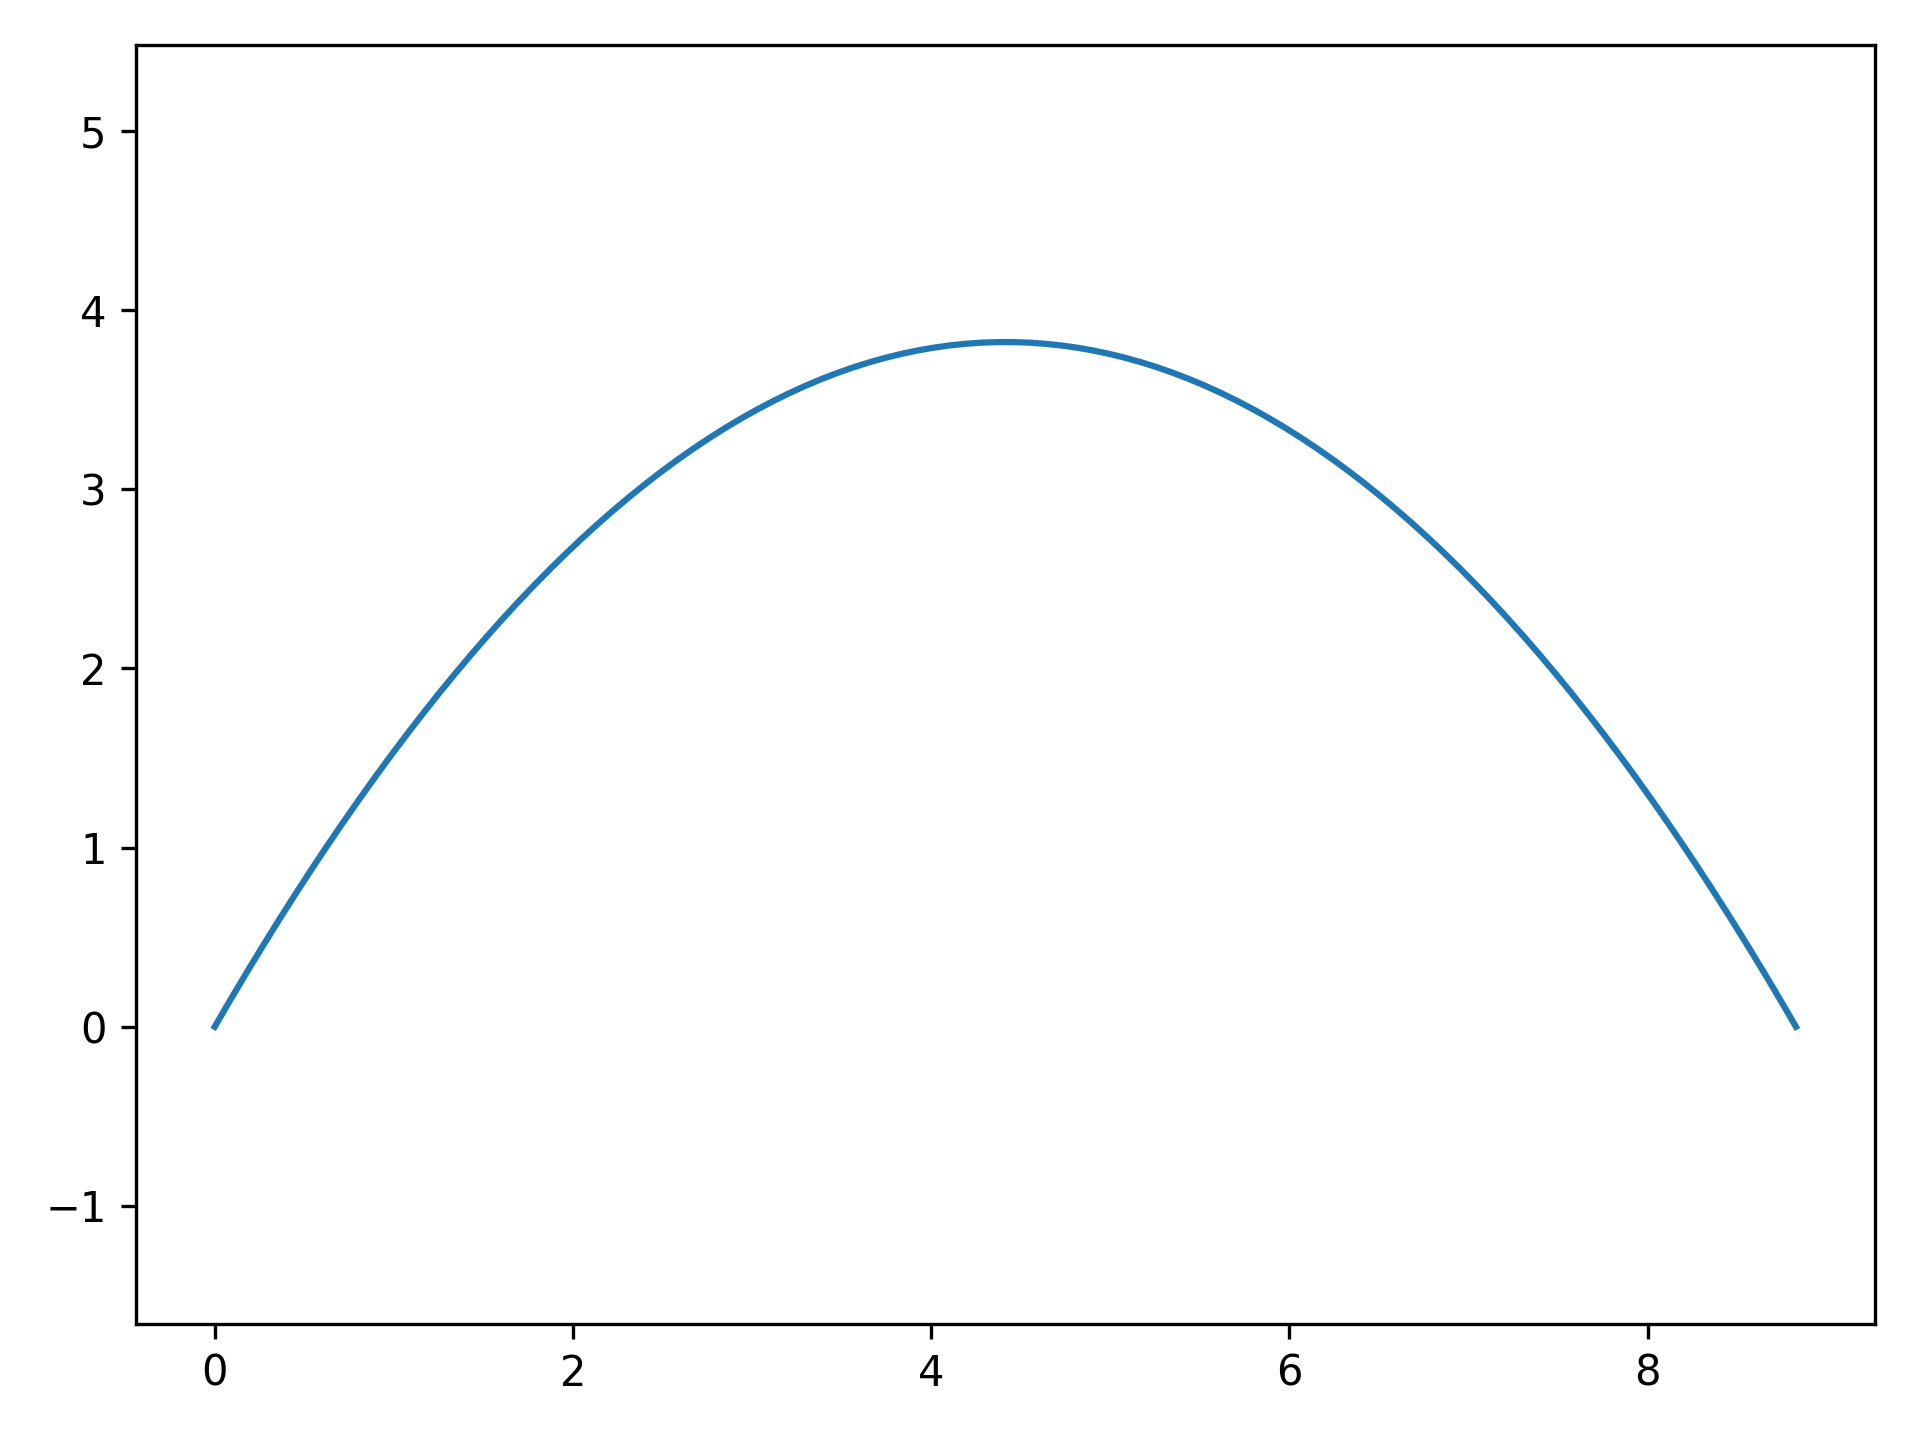
\includegraphics[scale=\myscale,scale=0.5]{figures/balle1}
\end{center}

Ci-dessous à gauche différents lancers pour différents angles mais une même vitesse initiale ; à droite différentes vitesses initiales pour un même angle.
\begin{center}
    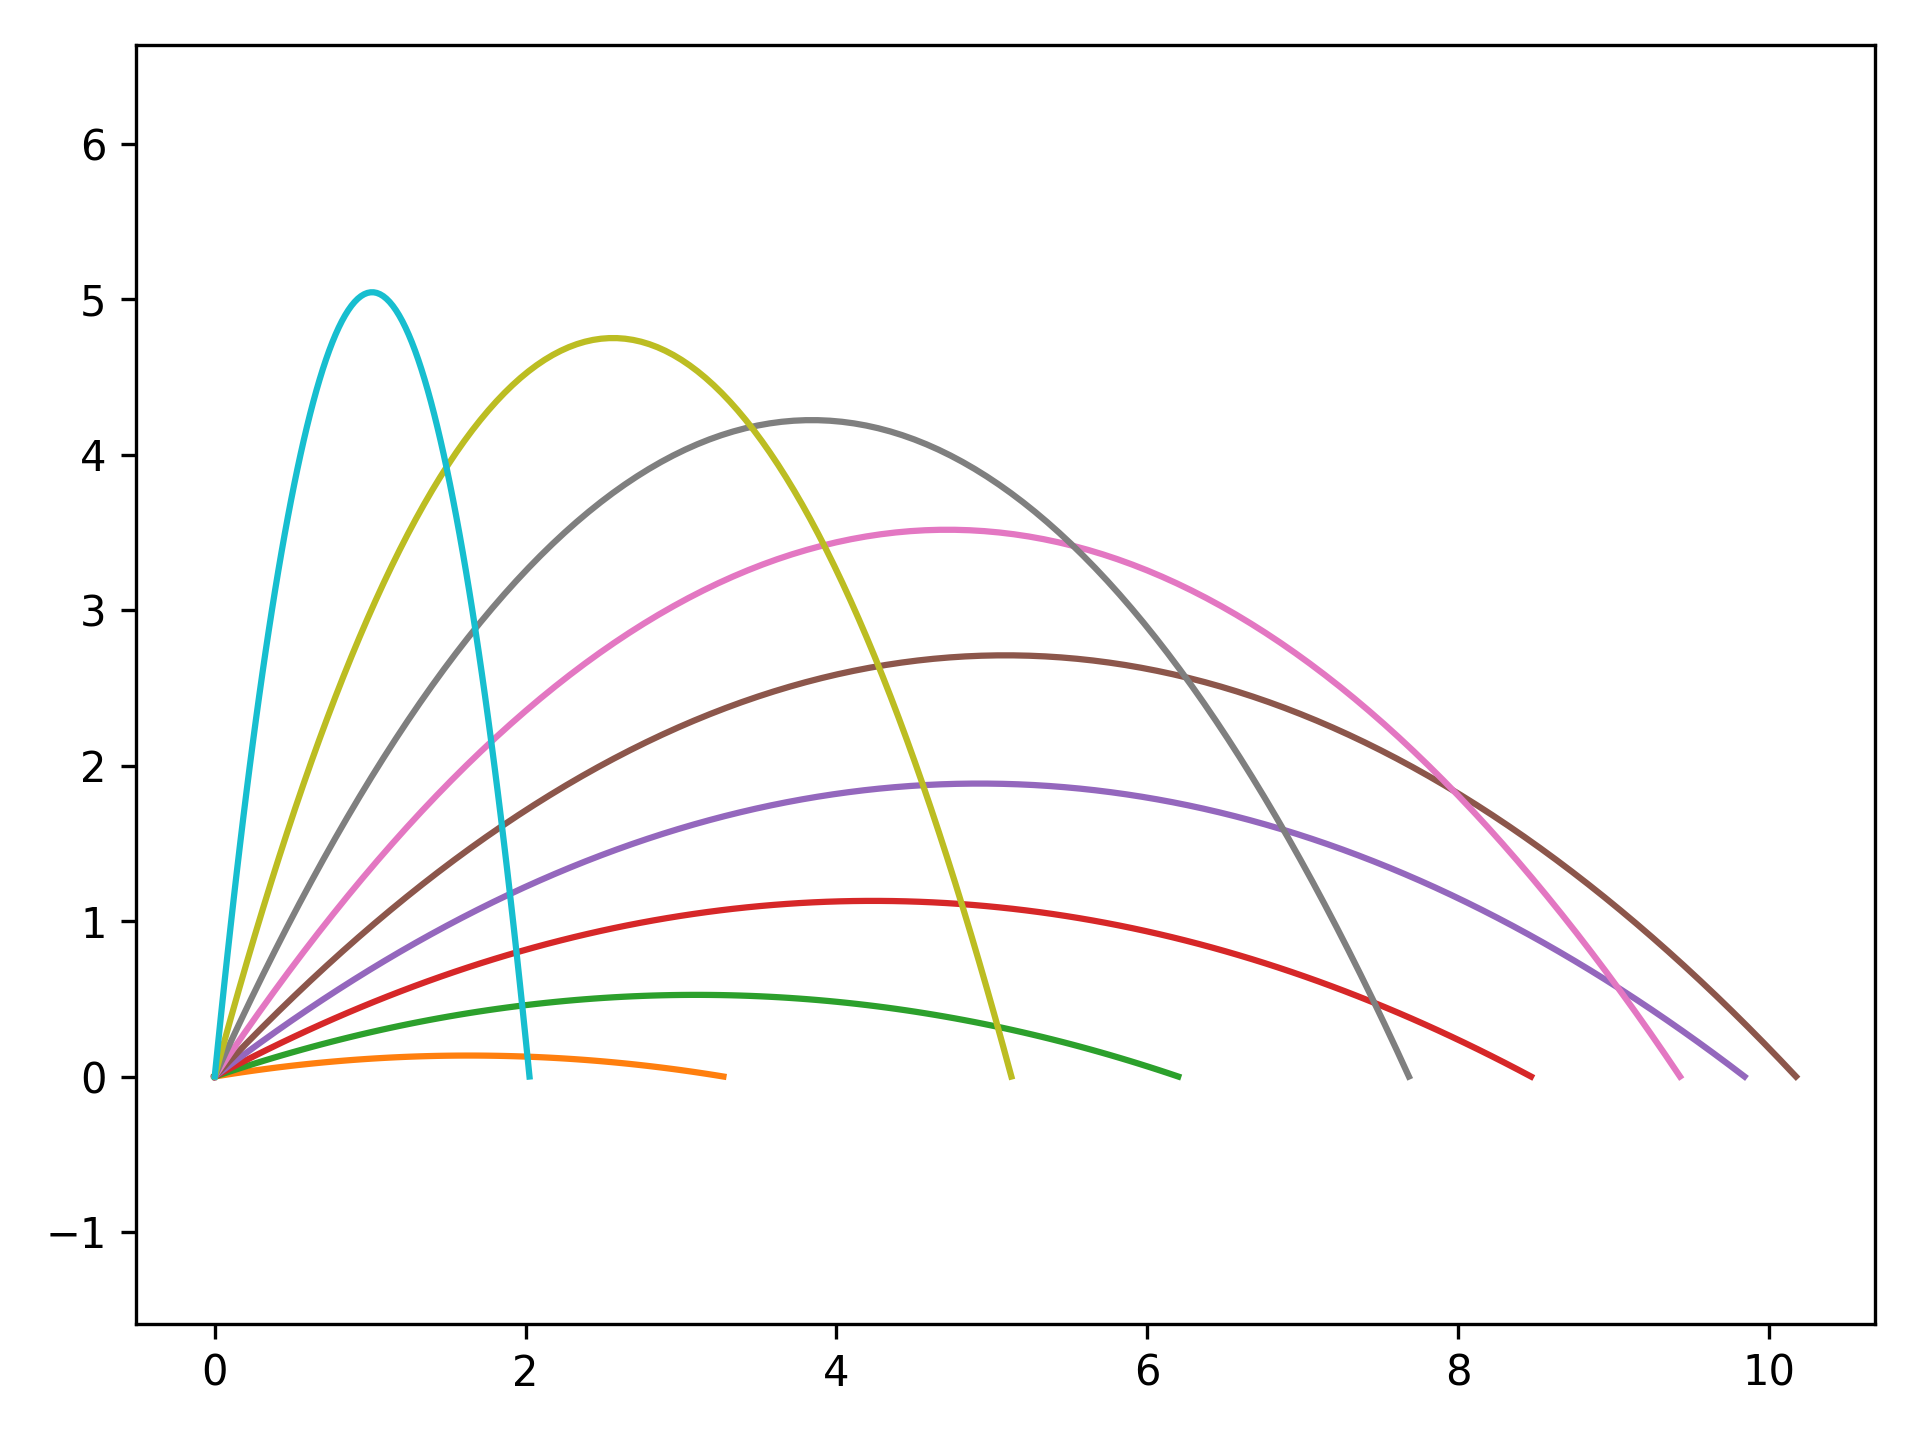
\includegraphics[scale=\myscale,scale=0.4]{figures/balle2}\qquad
    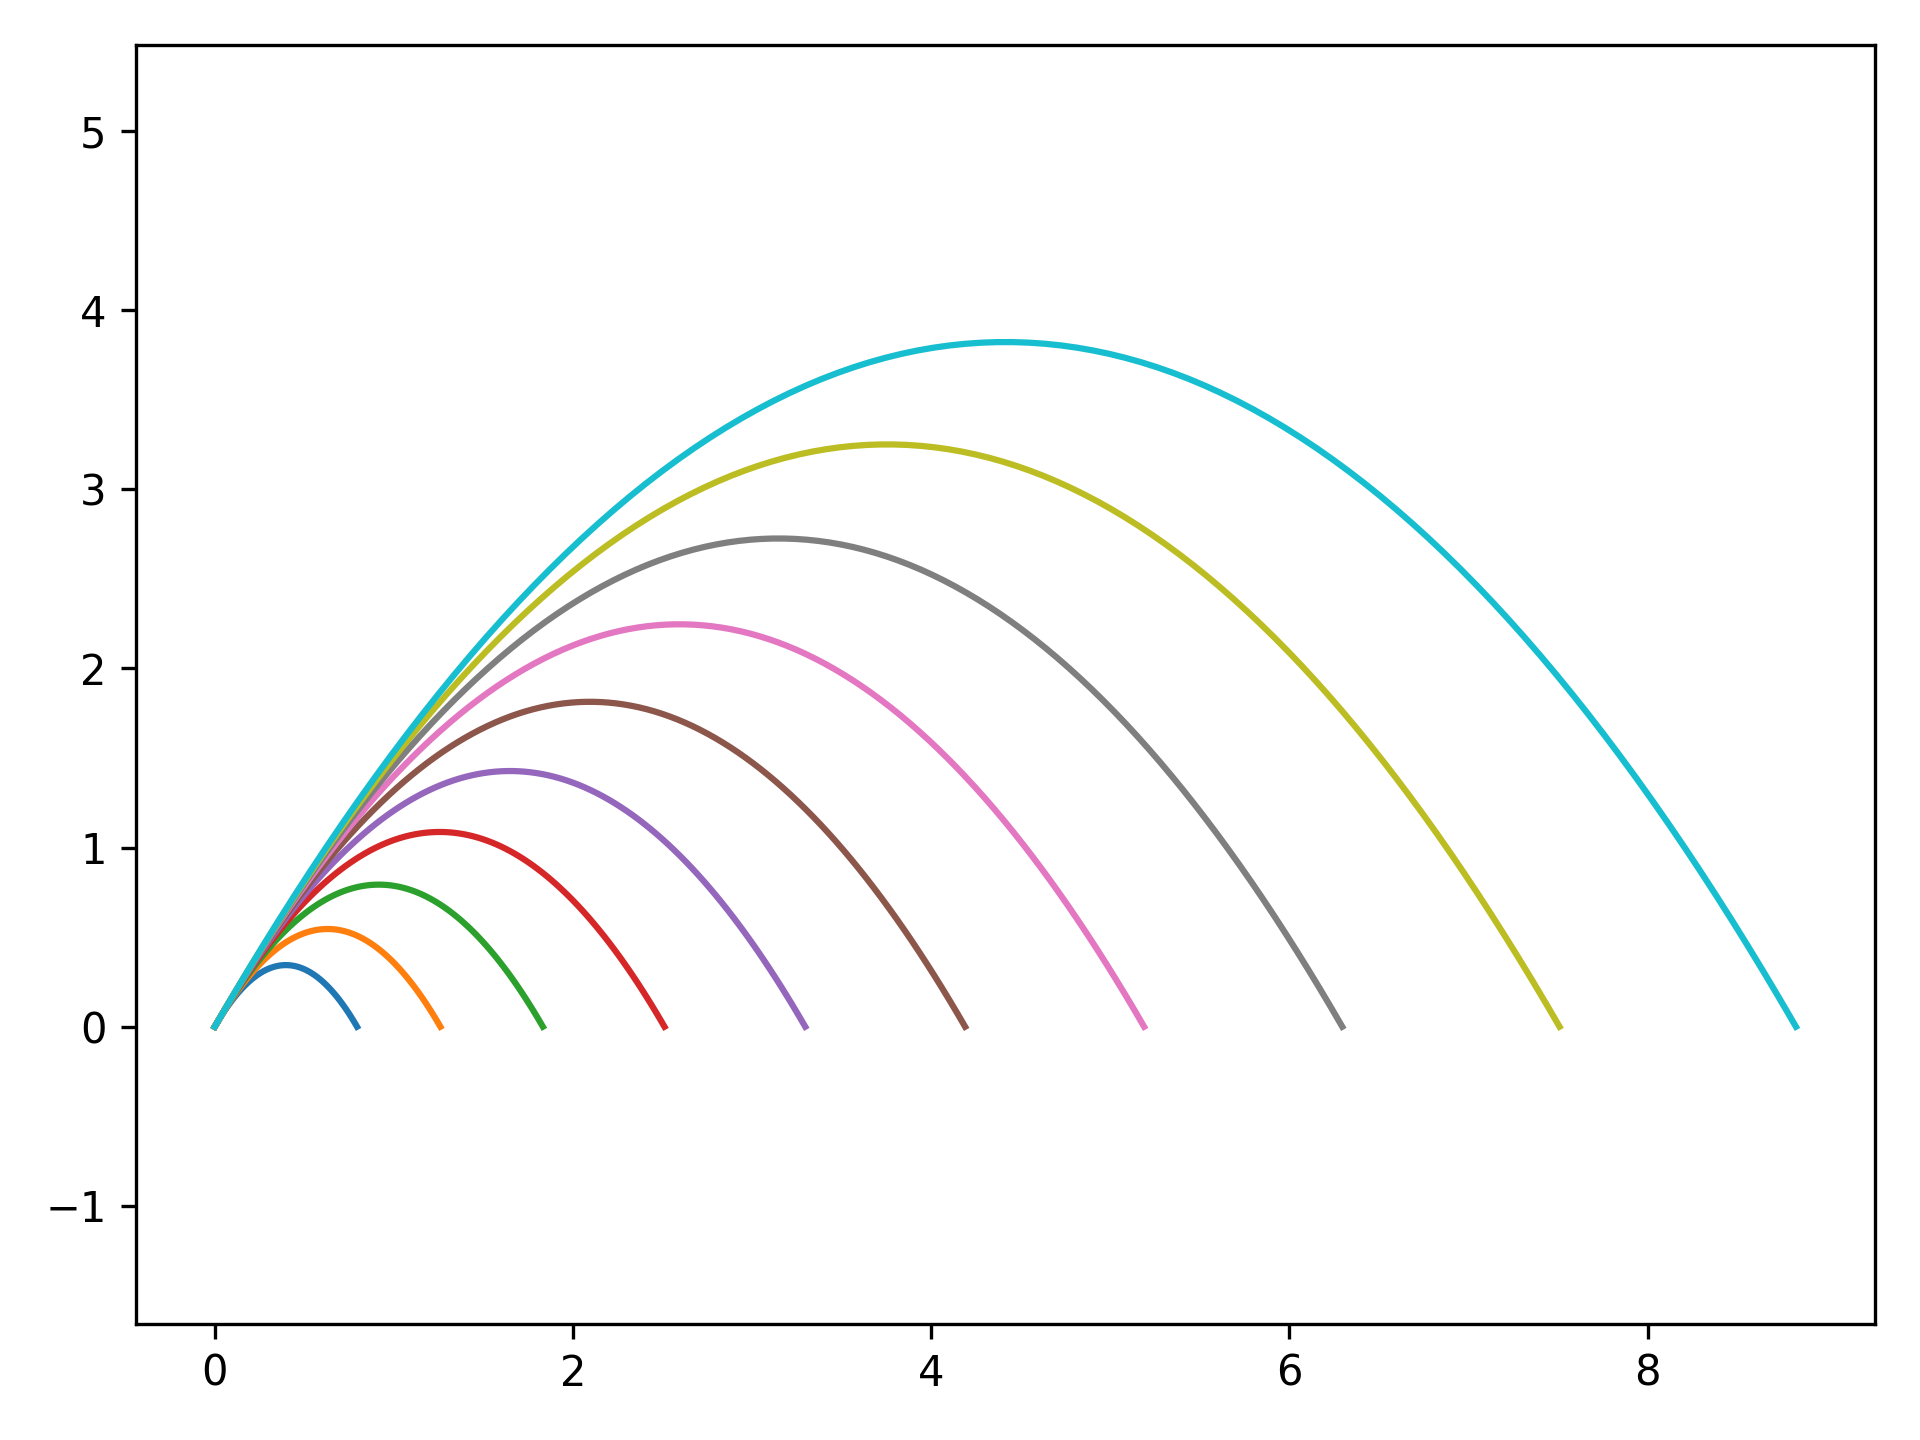
\includegraphics[scale=\myscale,scale=0.4]{figures/balle3}   
\end{center}

%--------------------------------------------------------------------
\subsection{Éléments différentiels}

 On va tracer la trajectoire pas à pas en utilisant les éléments différentiels (comme dans le chapitre \og{}Équations différentielles\fg). Si $(x(t) , y(t))$ est la position de la balle au temps $t$ et $(v_x(t), v_y(t))$ sa vitesse, alors on a $v_x(t) = \frac{x(t + \dd t) - x(t)}{\dd t}$ et $v_y(t) = \frac{y(t + \dd t) - y(t)}{\dd t}$.  
Ainsi la position à un temps $t + \dd t$ est donnée par :
\begin{align*}
    x(t + \dd t) &= x(t) + v_x(t) \dd t \\
    y(t + \dd t) &= y(t) + v_y(t) \dd t
\end{align*}
Mais comment calculer la vitesse ? La vitesse est la dérivée de la position donc $(v_x(t), v_y(t)) = (x''(t), y''(t))$.
Comme $x''(t)=0$ alors $x'(t)$ est constant et par condition initiale $v_x(t) = x'(t) = v_0 \cos \alpha$ est constant.
Par contre $y''(t) = -g$, donc $\frac{y'(t + \dd t) - y'(t)}{\dd t} = -g$ d'où $y'(t + \dd t) = y'(t) - g \dd t$ avec la condition initiale $y'(0) = v_0 \sin \alpha$.

On peut ainsi construire une trajectoire point par point.
On pose $(x_0, y_0) = (0, 0)$. On définit un intervalle élémentaire de temps $\dd t$ (par exemple $\dd t = 0.01$).  La formule de récurrence est alors :
\begin{align*}
    x_{n+1} &= x_n + v_0  \cos(\alpha) \dd t \\
    y_{n+1} &= y_n + v_{y,n} \sin(\alpha) \dd t \\
    v_{y,n+1} &= v_{y,n} - g \dd t
\end{align*}

\bigskip

Il est rarement facile de  pouvoir expliciter les solutions d'une équation différentielle. Par exemple, ajoutons une force de frottement qui s'oppose au mouvement de la balle. Cette force de résistance est donnée en fonction de la vitesse
$$\vec R = -k \| \vec v\| ^{e} \frac{\vec v}{\| \vec v \|}$$
$k$ est une constante. Des modèles classiques pour l'exposant sont $e=1$ (la résistance est proportionnelle à la vitesse, valable pour une vitesse faible) ou bien $e=2$ (la résistance est proportionnelle au carré de la vitesse), des valeurs non entières de $e$ sont aussi intéressantes.
Le principe fondamental de la mécanique $\vec P + \vec R = m\vec g$ conduit à des équations différentielles plus compliquées, voire impossibles à résoudre par des formules analytiques. Cependant en utilisant la méthode des éléments différentiels (\emph{aka} la méthode d'Euler) on trace facilement les trajectoires.
On pose $(x_0, y_0) = (0, 0)$, $(v_{x,0}, v_{y,0}) = (v_0 \cos \alpha, v_0 \sin \alpha)$.
La formule de récurrence est : 
\begin{align*}
	x_{n+1} &= x_n + v_{x,n} \dd t \\
	y_{n+1} &= y_n + v_{y,n} \dd t \\
	\theta_n &= \arctantwo(v_{y,n},v_{x,n}) \\ 
	\| \vec{v_n} \| &= \sqrt{v_{x,n}^2 + v_{y,n}^2} \\
	v_{x,n+1} &= v_{x,n} - \frac{k}{m} 	\| \vec{v_n} \|^e \cos \theta_n \dd t \\     
	v_{y,n+1} &= v_{y,n} - g \dd t - \frac{k}{m} \| \vec{v_n} \|^e \sin \theta_n \dd t \\
\end{align*}



\myfigure{0.7}{
	\tikzinput{fig-balle-02}
}

$\theta_n$ est l'angle formé par le vecteur vitesse et l'horizontale.
Noter que cette fois-ci la masse intervient dans les équations.
Ci-dessous une trajectoire avec frottement quadratique ($e=2$\couleurnb{ en rouge}{}) comparée à une trajectoire sans frottement. La courbe avec frottement n'est plus une parabole.

\begin{center}
	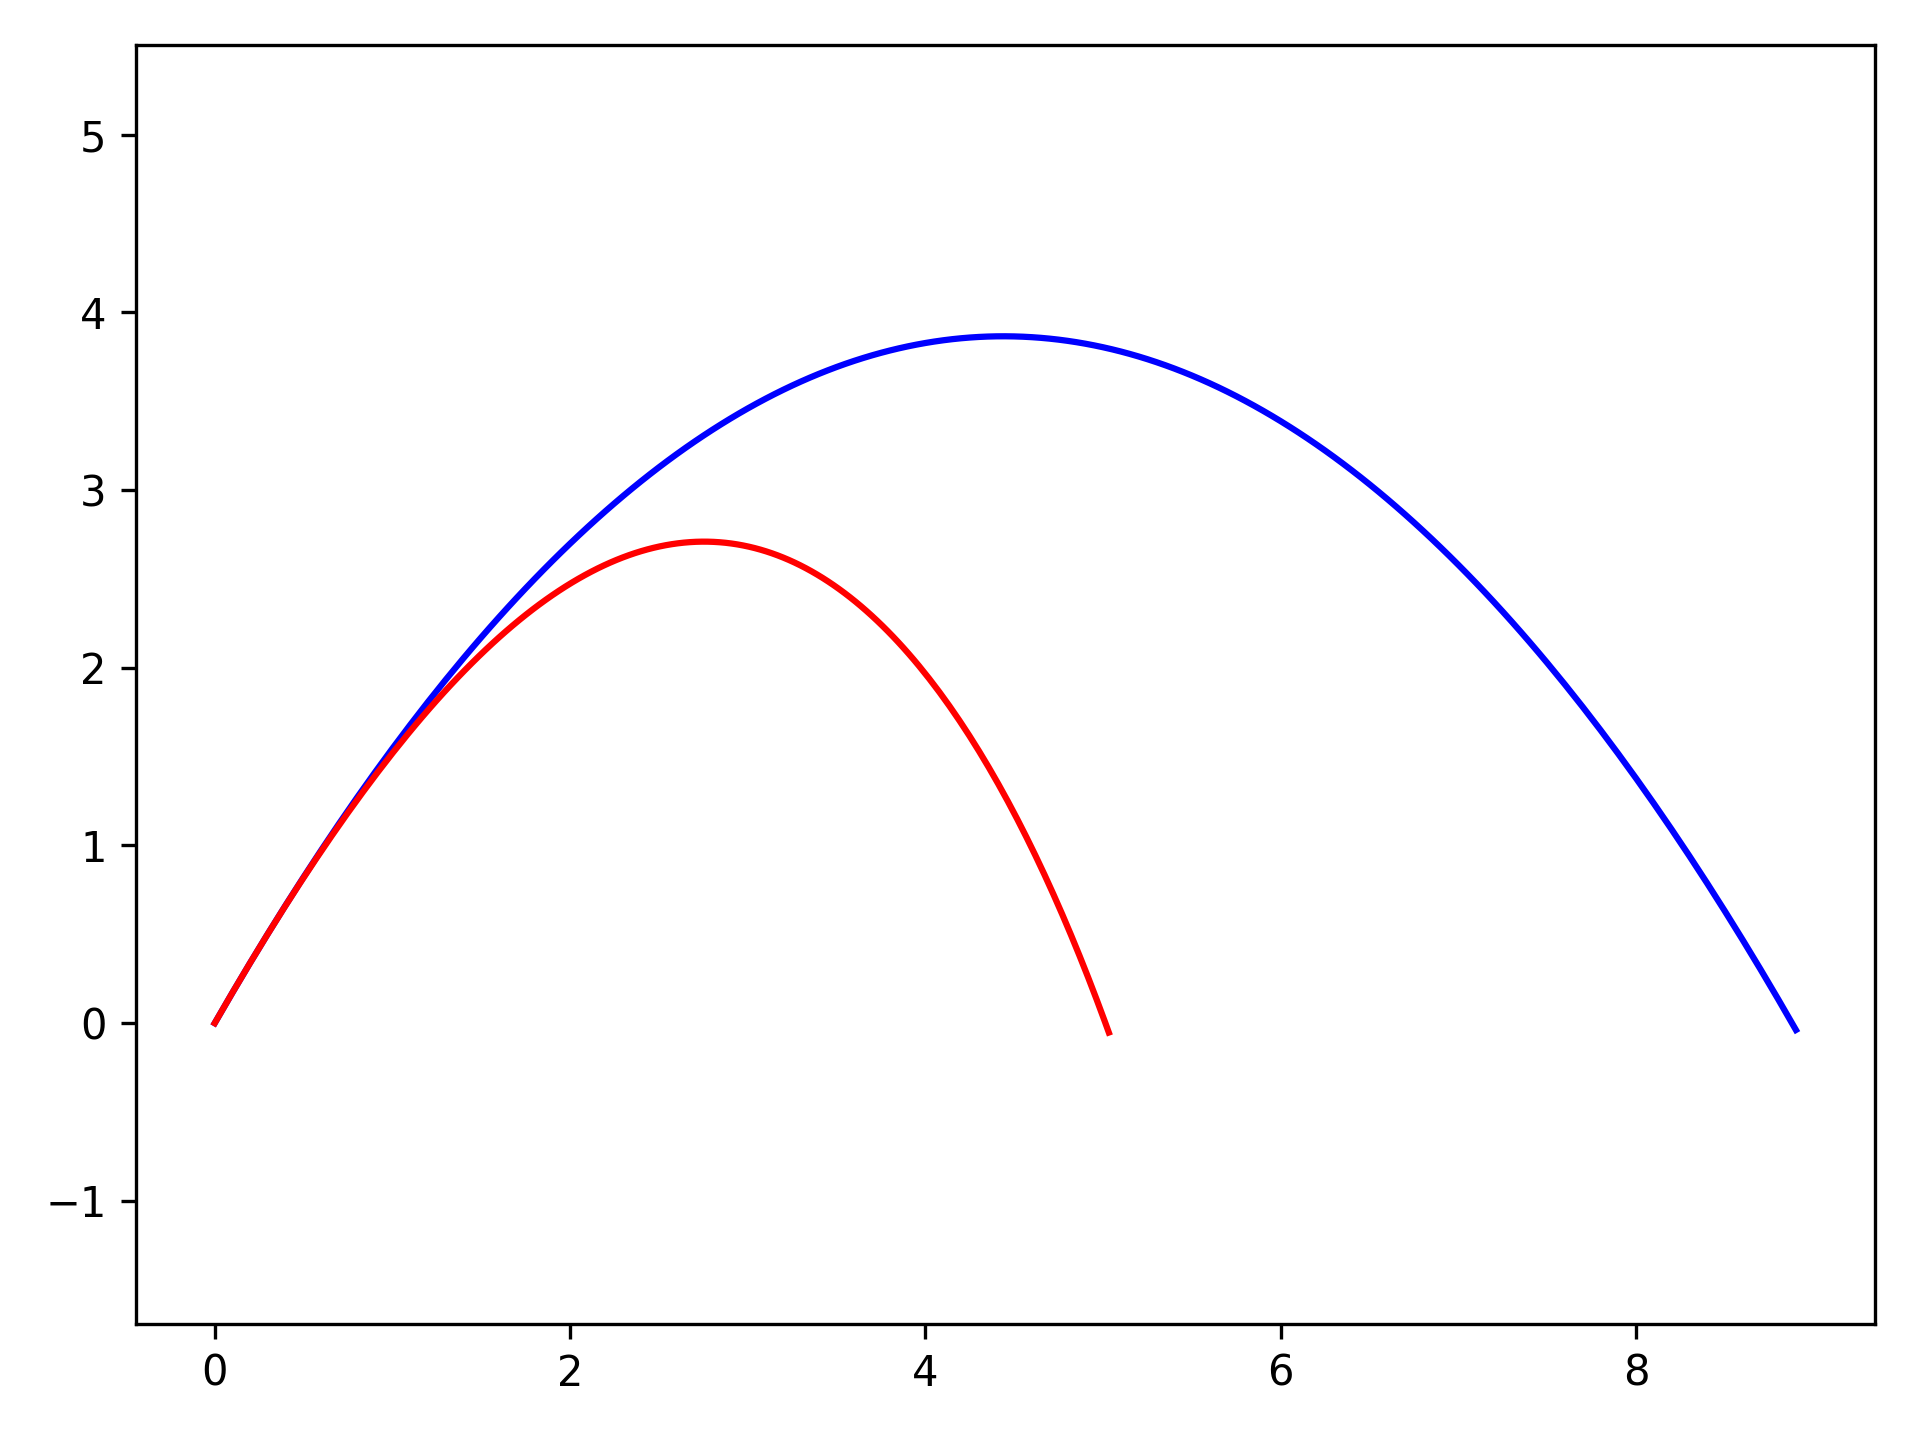
\includegraphics[scale=\myscale,scale=0.5]{figures/balle-frottements}
\end{center}


%--------------------------------------------------------------------
\subsection{Rebonds}

Il est facile de modéliser un rebond. Par exemple dès que l'ordonnée $y$ de la balle devient négative, on simule un nouveau lancer de balle. Afin de modéliser la perte d'énergie au fur et à mesure des rebonds, la vitesse du lancer au rebond numéro $k$ diminue à chaque rebond selon une formule $v_{k+1} = c v_k$, avec une vitesse initiale $v_0$ et un coefficient $0 \le c \le 1$ (par exemple $c=0.8$).

\begin{center}
	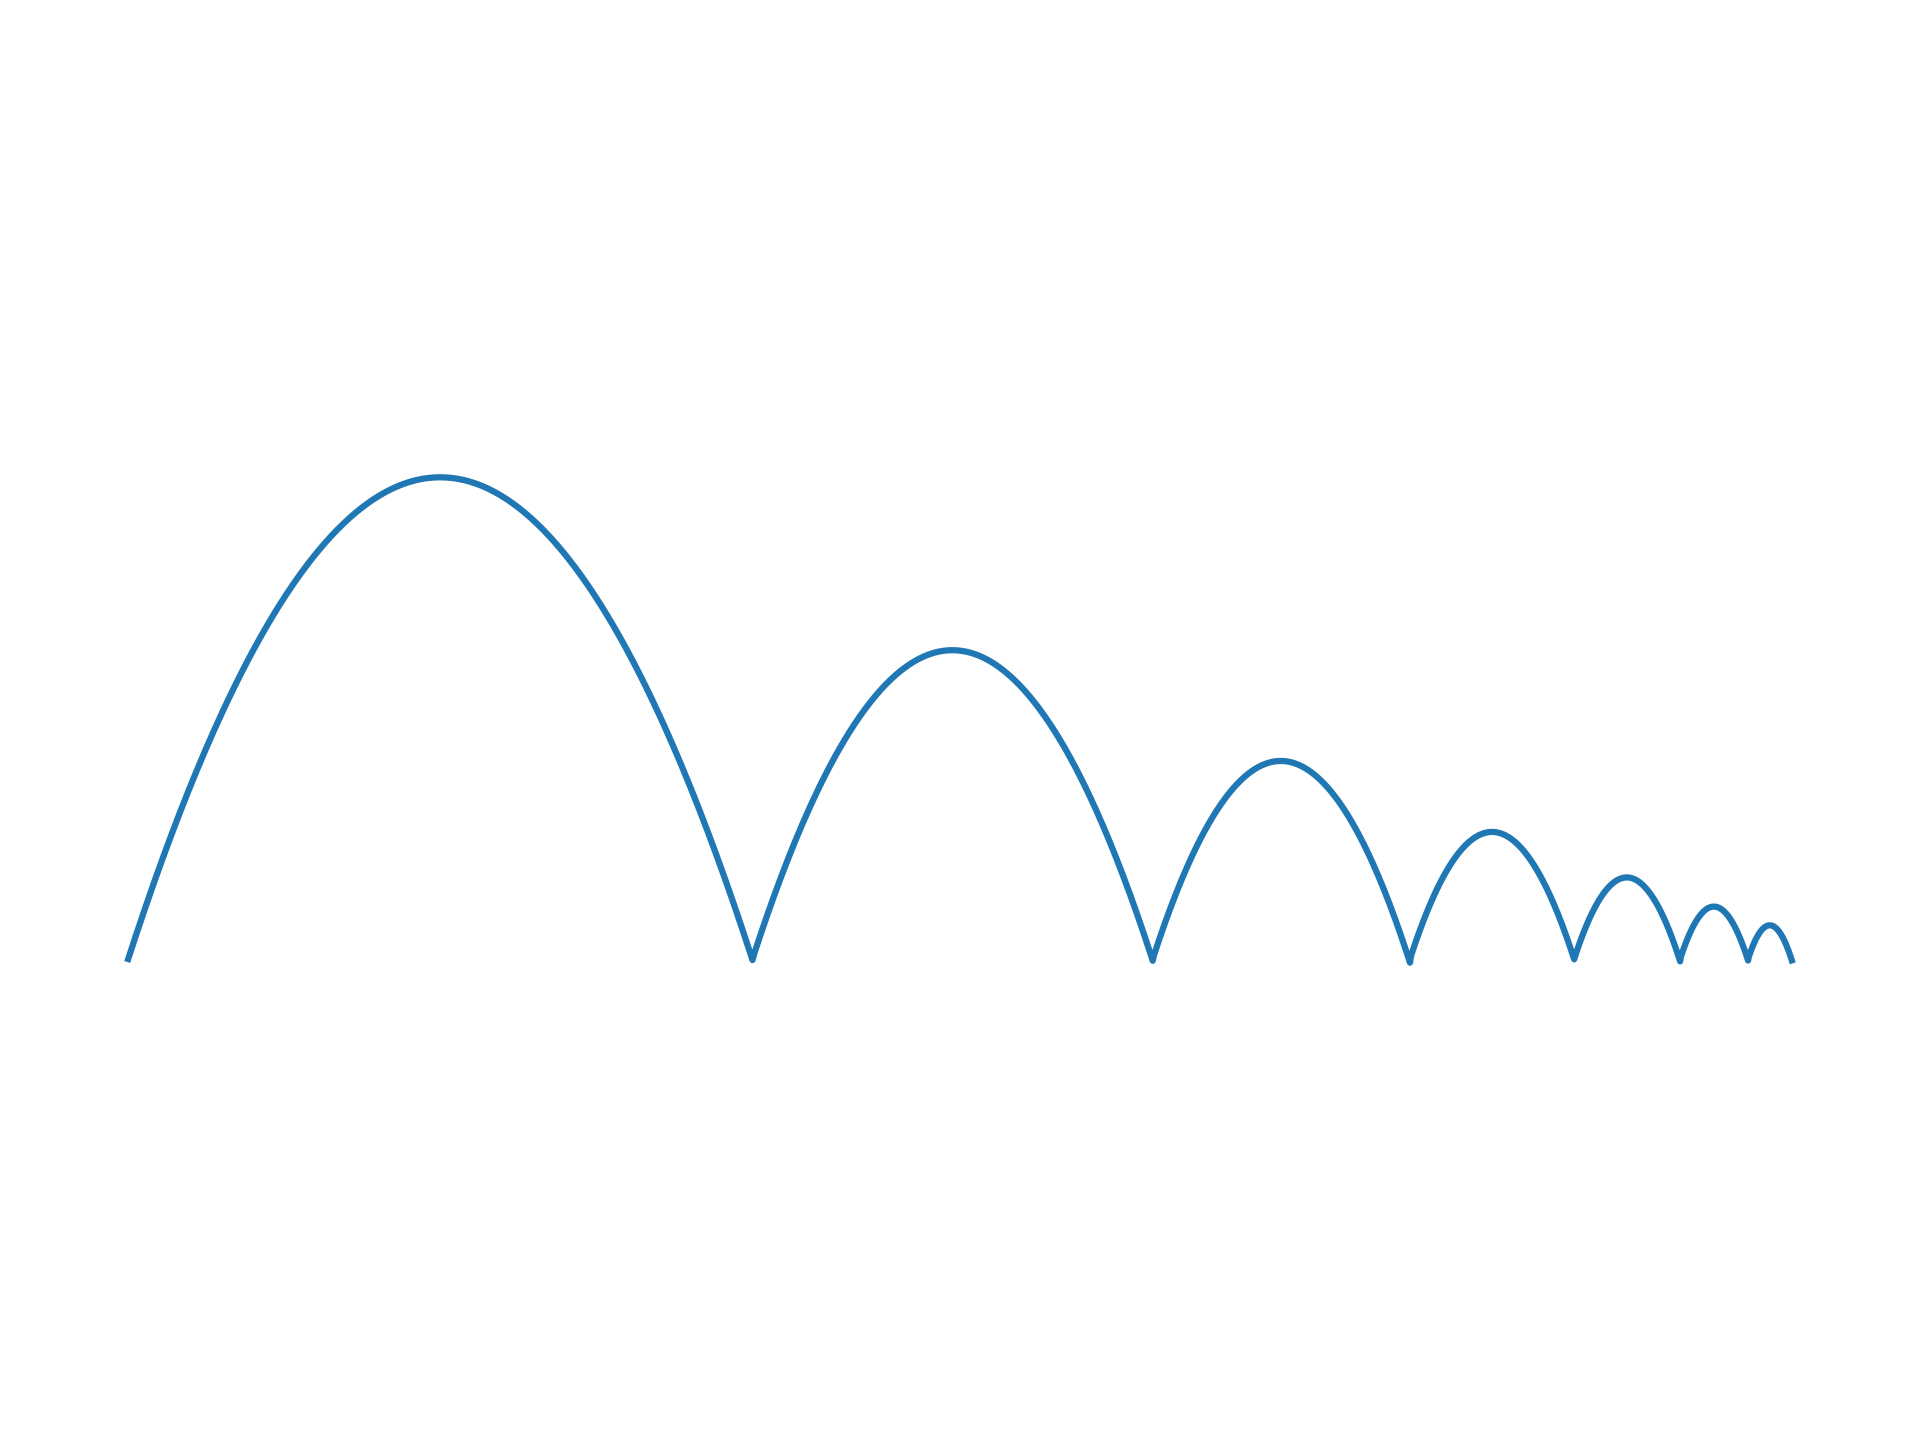
\includegraphics[scale=\myscale,scale=0.5,trim={0 3cm 0 3cm},clip]{figures/balle-rebond}
\end{center}



%%%%%%%%%%%%%%%%%%%%%%%%%%%%%%%%%%%%%%%%%%%%%%%%%%%%%%%%%%%%%%%%%%%%%
\section{Ondes}

\index{onde}

%--------------------------------------------------------------------
\subsection{Une dimension}

Une onde est le déplacement d'une perturbation d'une propriété physique par rapport à son état d'équilibre.
Par exemple une onde sonore est une modification de la pression de l'air : des particules d'air sont comprimées par la source sonore, elles vont perturber les particules voisines qui à leur tour perturbent d'autres particules.

\begin{center}
	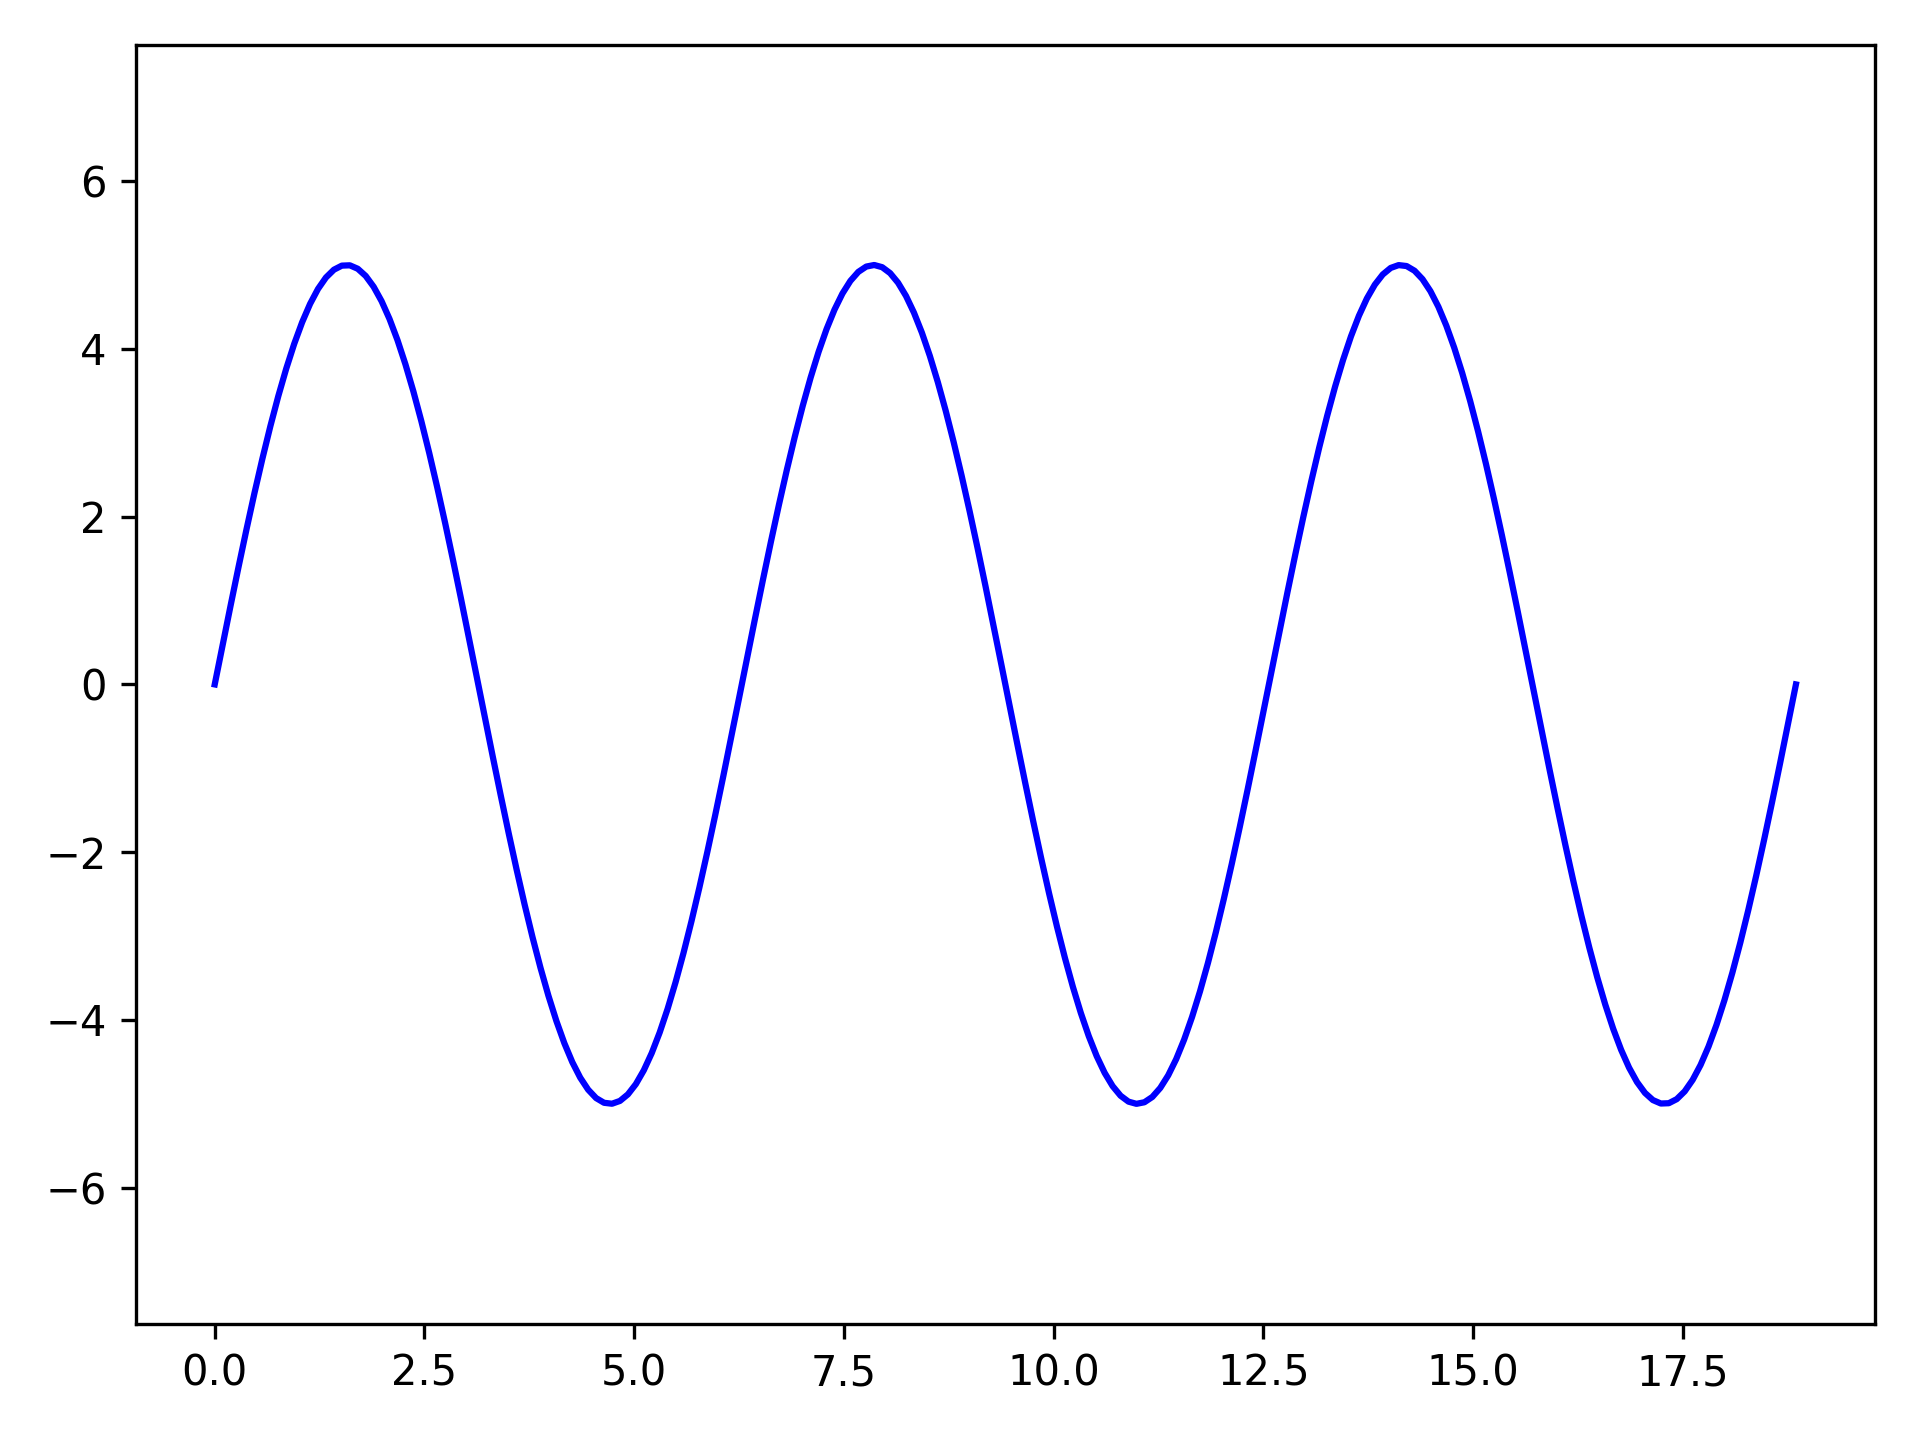
\includegraphics[scale=\myscale,scale=0.5]{figures/ondes1D-1}
\end{center}

Beaucoup de phénomènes, comme des vagues par exemple, sont modélisés par des ondes sinusoïdales. L'équation est 
$$F(x,t) = A \sin\left(\frac{2\pi}{\lambda} x -  \frac{2\pi}{T} t\right)$$
où 
\begin{itemize}
	\item $F(x,t)$ représente une propriété physique,
	\item en fonction d'une position $x\in\Rr$,
	\item et d'un instant $t$,
	\item $A$ est l'amplitude,
	\item $\lambda$ est la longueur d'onde,
	\item $T$ est la période.
\end{itemize}

La longueur d'onde $\lambda$ mesure la distance (en mètre) entre deux crêtes d'une même sinusoïde. 
L'onde se décale vers la droite au fil du temps, son graphe se superpose à lui-même au bout de $T$ secondes.
La vitesse de l'onde se calcule par $v = \frac{\lambda}{T}$. 

\begin{center}
	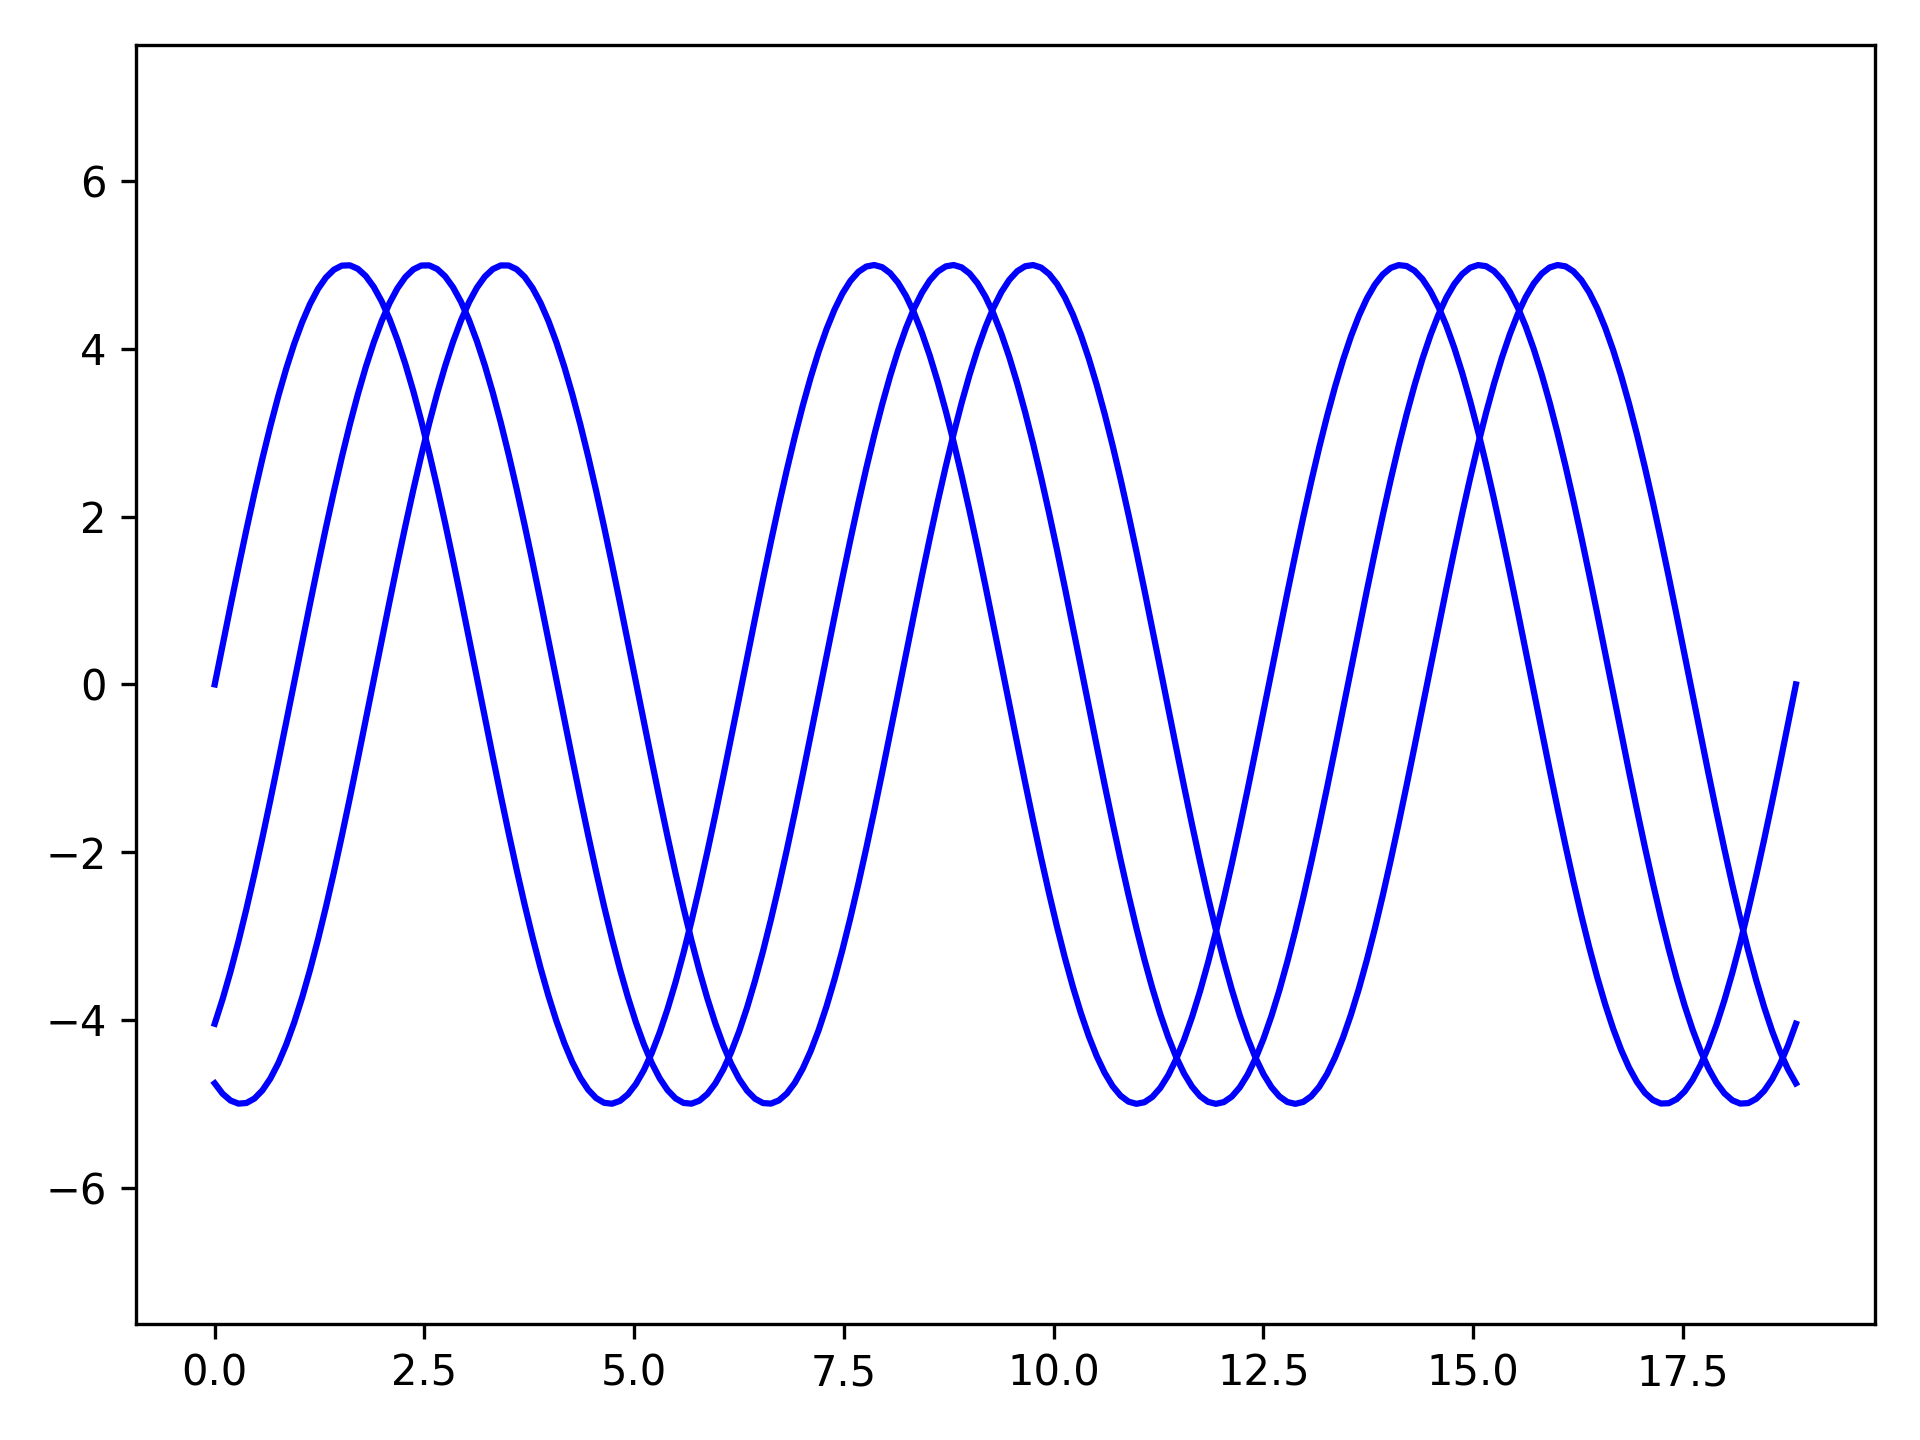
\includegraphics[scale=\myscale,scale=0.5]{figures/ondes1D-2}
\end{center}


Lorsque l'on superpose deux ondes sinusoïdales $F_1(x,t) + F_2(x,t)$ ayant des caractéristiques différentes, on obtient des fonctions plus compliquées. Ci-dessous les graphes de deux ondes $F_1$ et $F_2$ (en haut) ainsi que leur superposition $F_1+F_2$ (en bas).

\begin{center}
	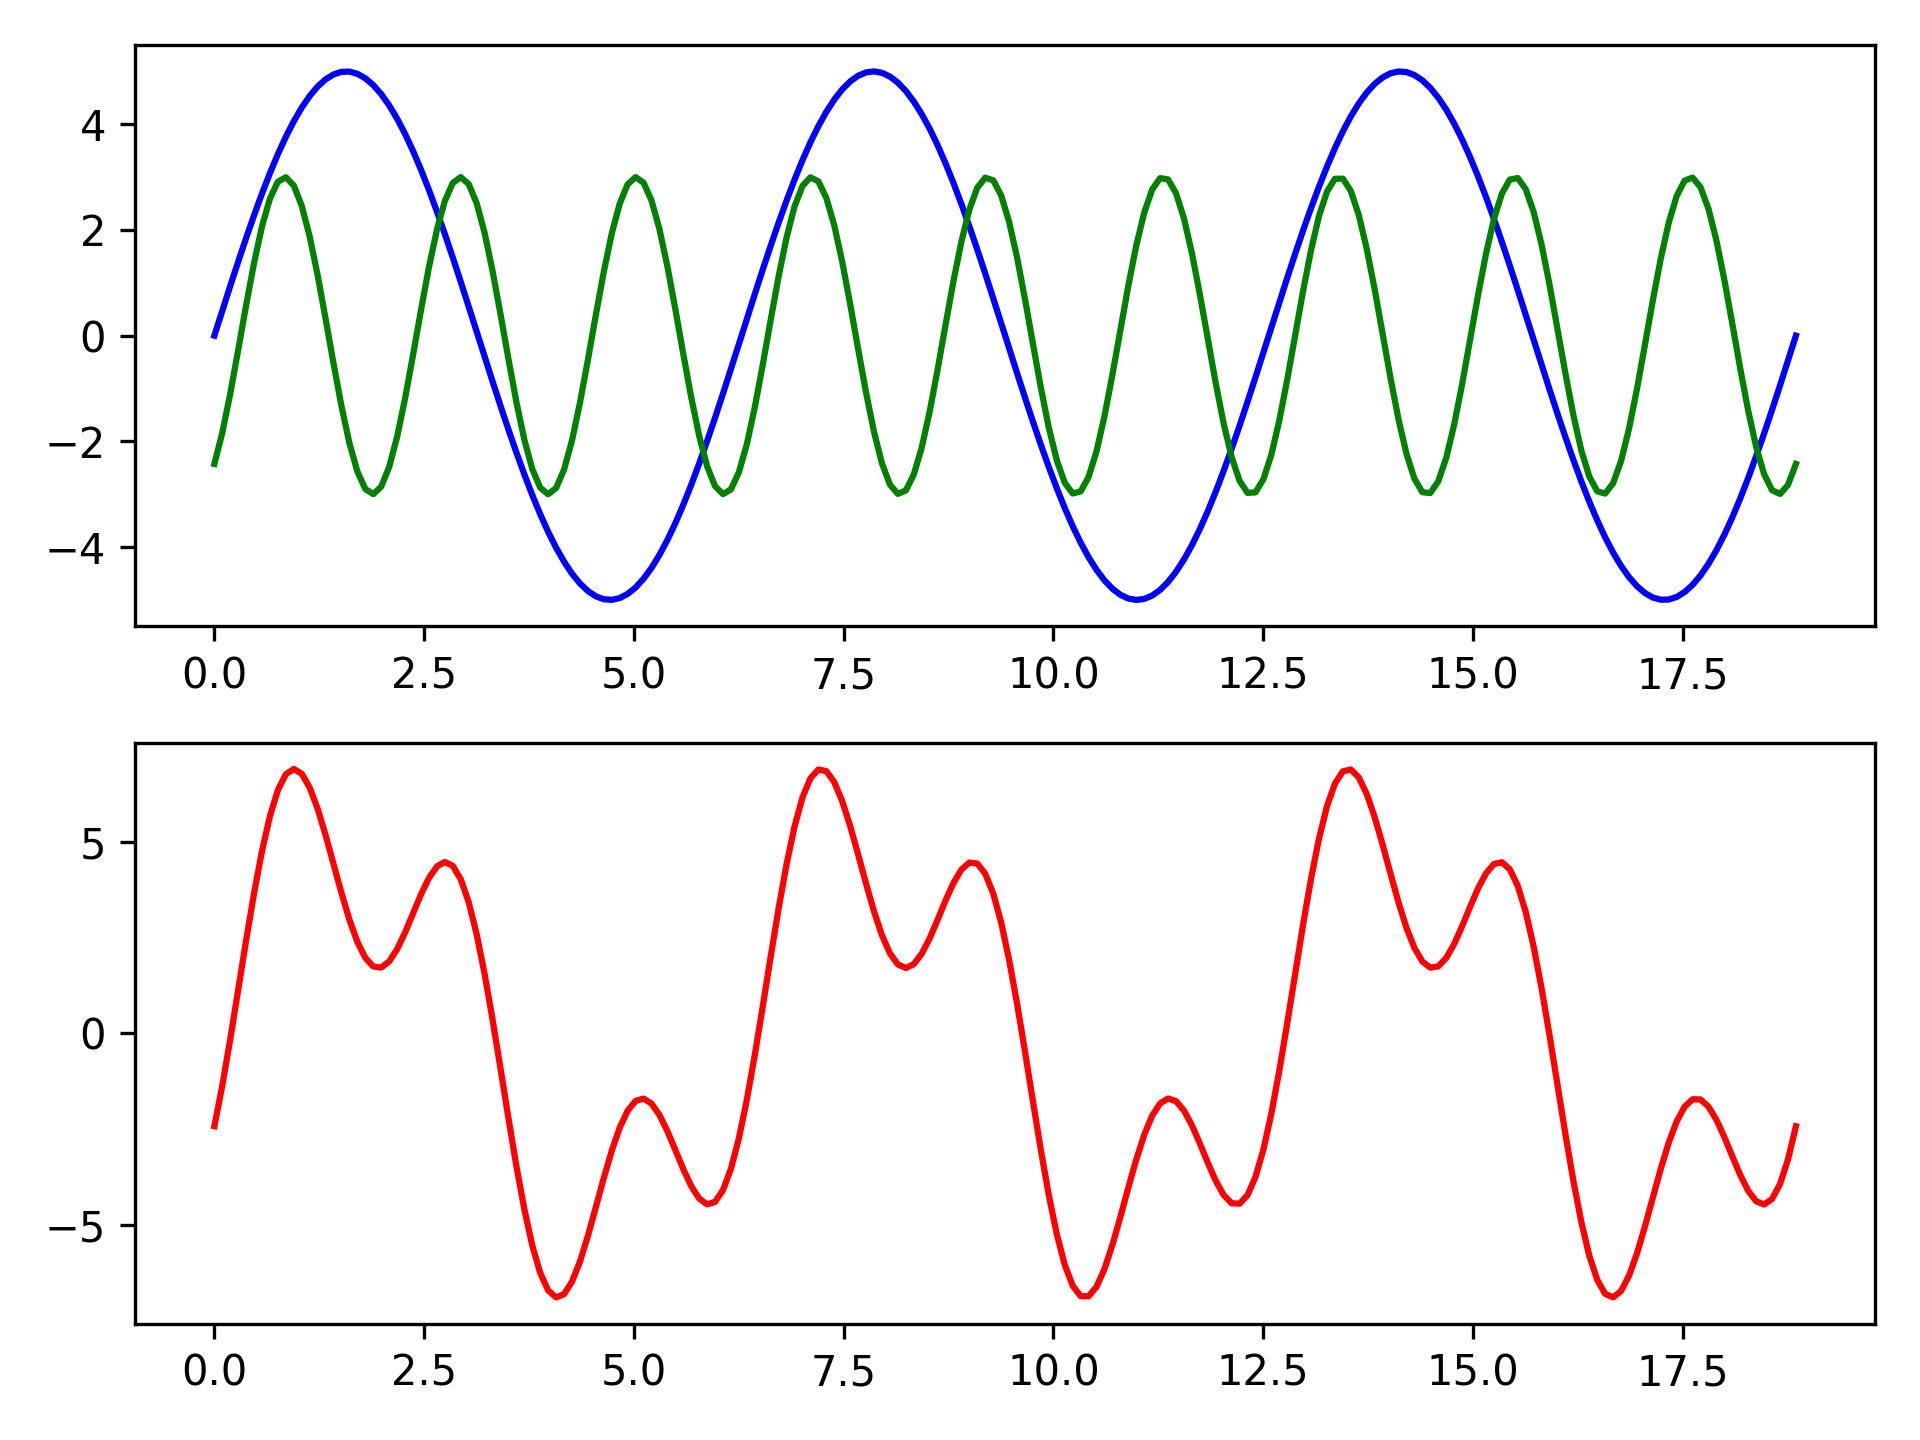
\includegraphics[scale=\myscale,scale=0.5]{figures/ondes_superposition}
\end{center}


%--------------------------------------------------------------------
\subsection{Deux dimensions}

Lorsque qu'une pierre tombe dans l'eau, cela entraîne  une onde à la surface sous la forme de cercles qui s'agrandissent. Par contre, la hauteur des vagues diminue lorsque l'on s'éloigne de la source car une même énergie se répartit dans toutes les directions.

\begin{center}		
	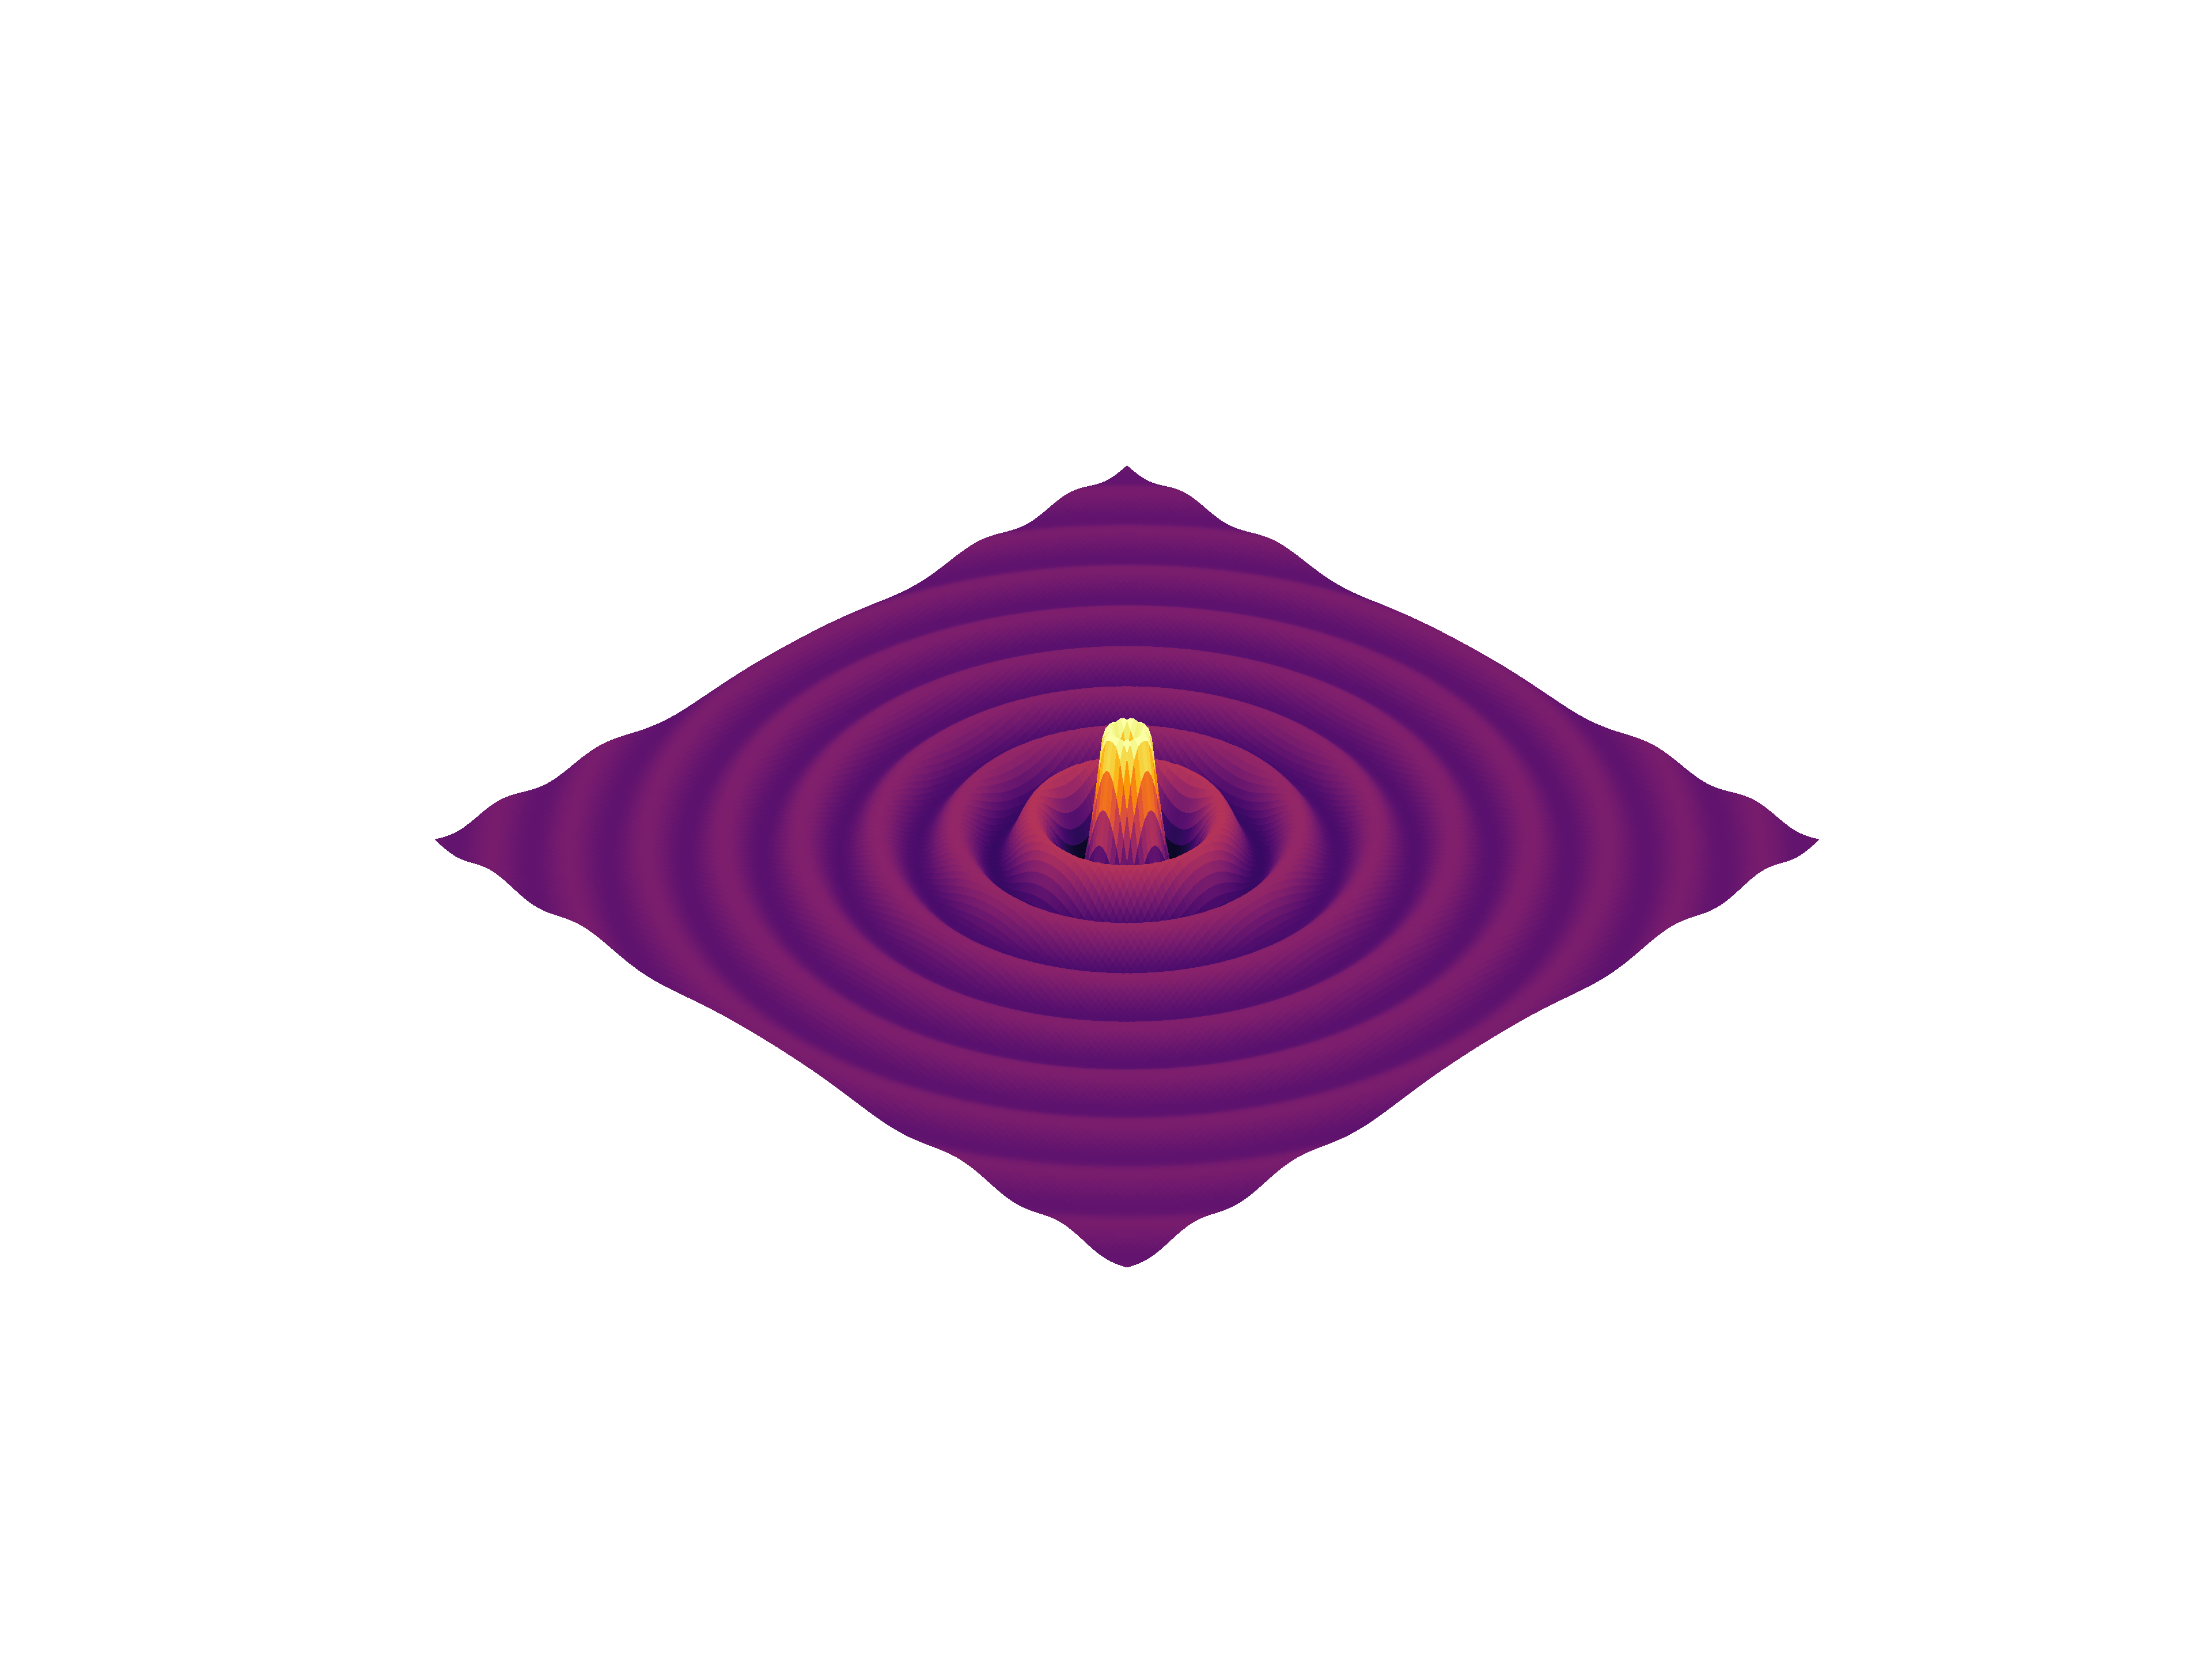
\includegraphics[scale=\myscale,scale=0.8,trim={0 2.5cm 0 3cm},clip]{figures/ondes2D-2}	
\end{center}

La formule correspondante est :
$$F(r,t) = \frac{A}{r} \sin\left(\frac{2\pi}{\lambda} r -  \frac{2\pi}{T} t\right)$$
où $r = \sqrt{x^2+y^2}$ mesure la distance à l'origine.

Voici l'allure d'une tranche selon le plan $(y=0)$.
\begin{center}
	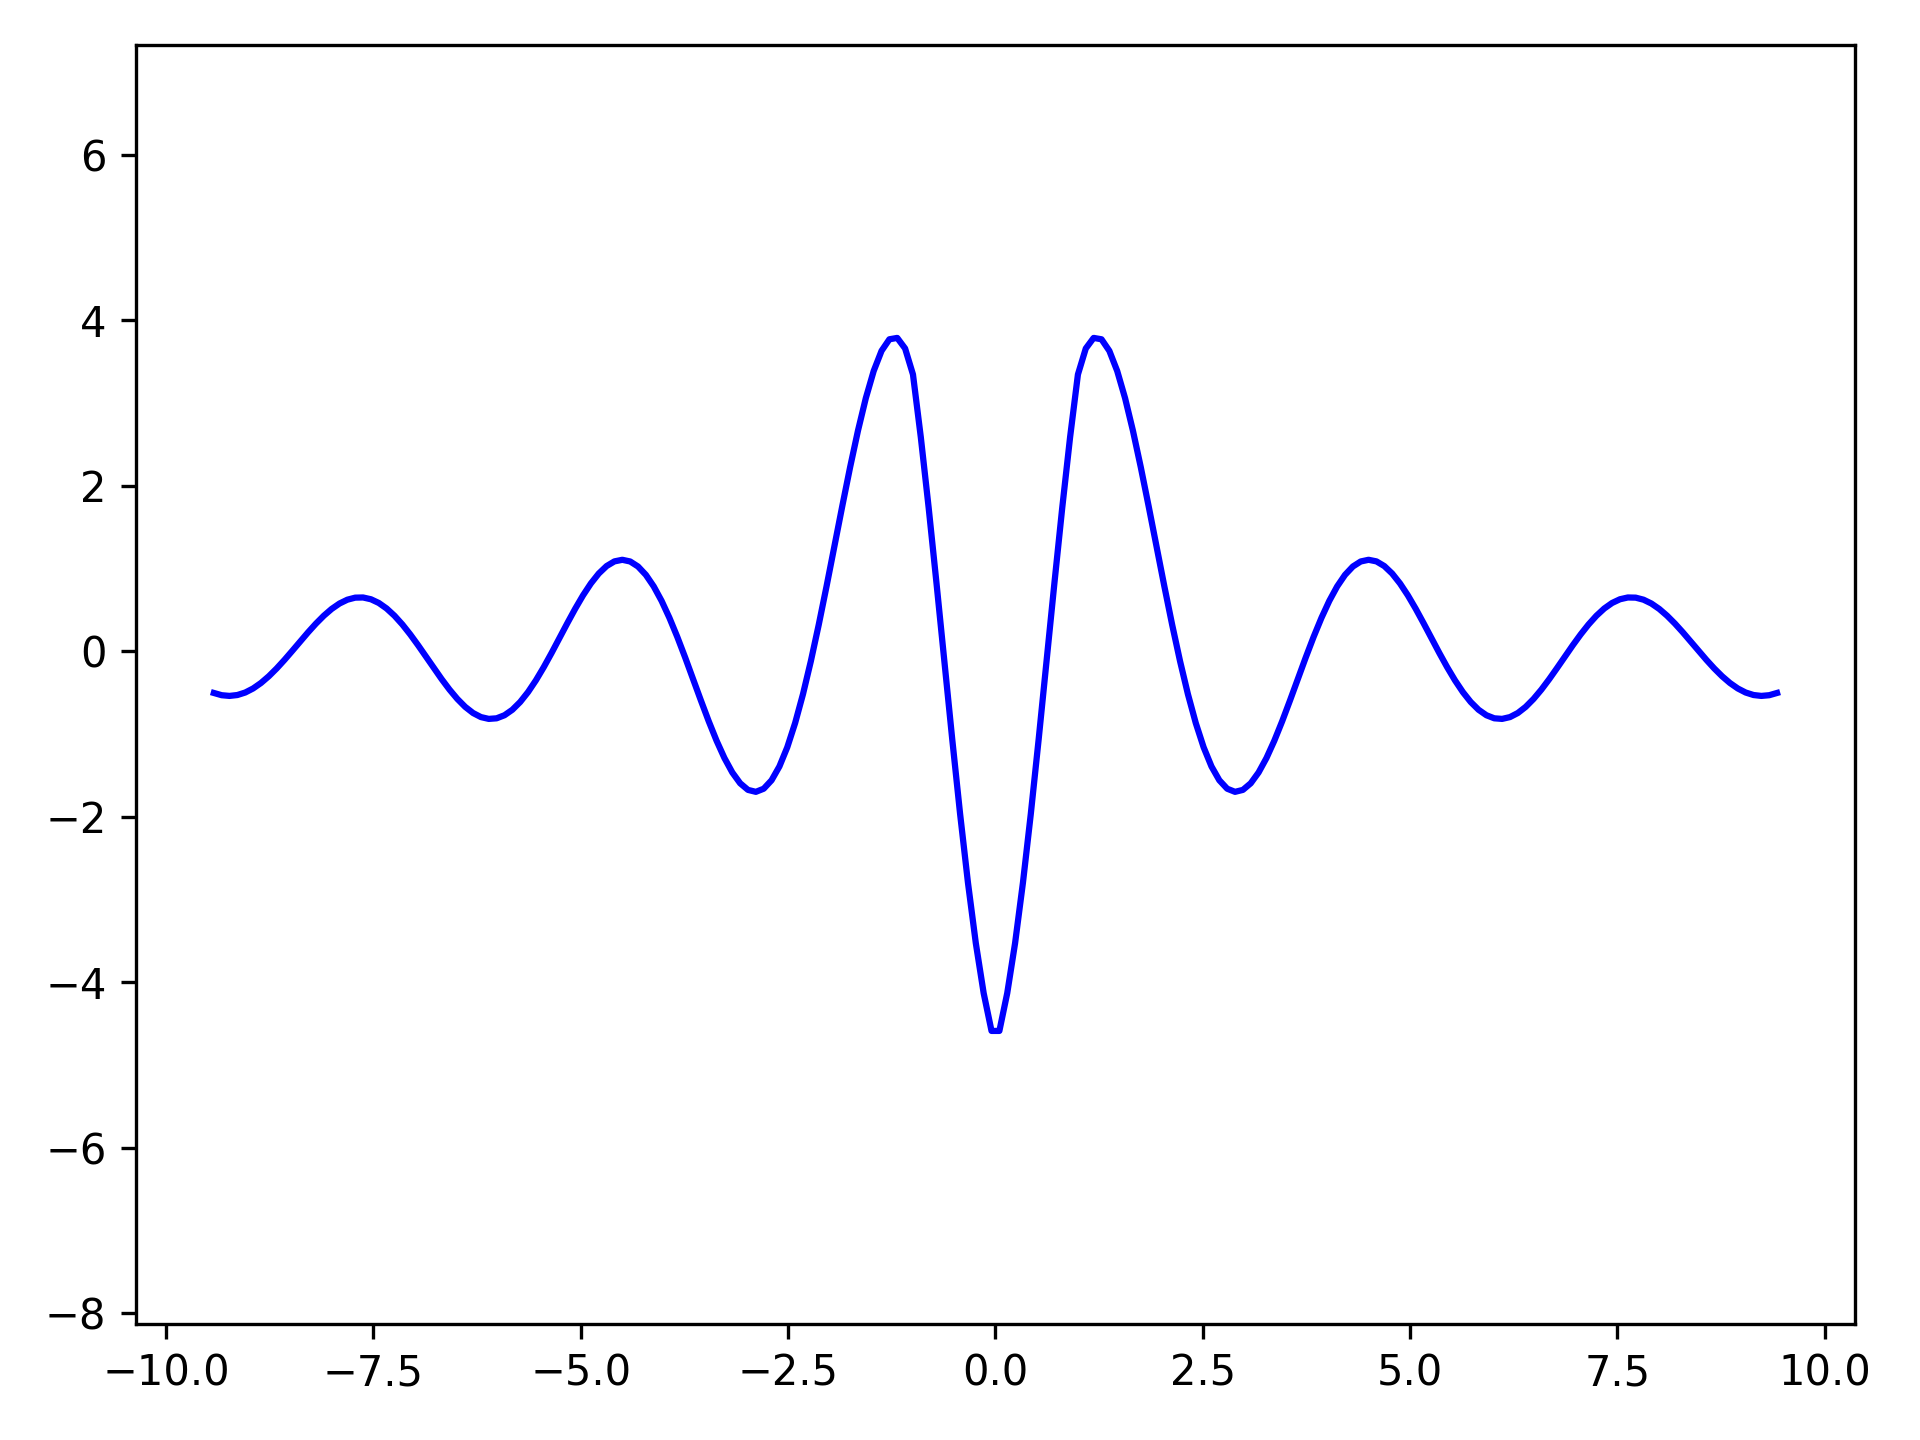
\includegraphics[scale=\myscale,scale=0.4]{figures/ondes2D-1}
\end{center}


Il est intéressant de lancer deux pierres en même temps vers des points différents. 
Les ondes se superposent et on voit apparaître des interférences, par exemple des zones où la hauteur des vagues est nulle (la crête issue de la première pierre est compensée par le creux issu de la seconde pierre et réciproquement).
\begin{center}
	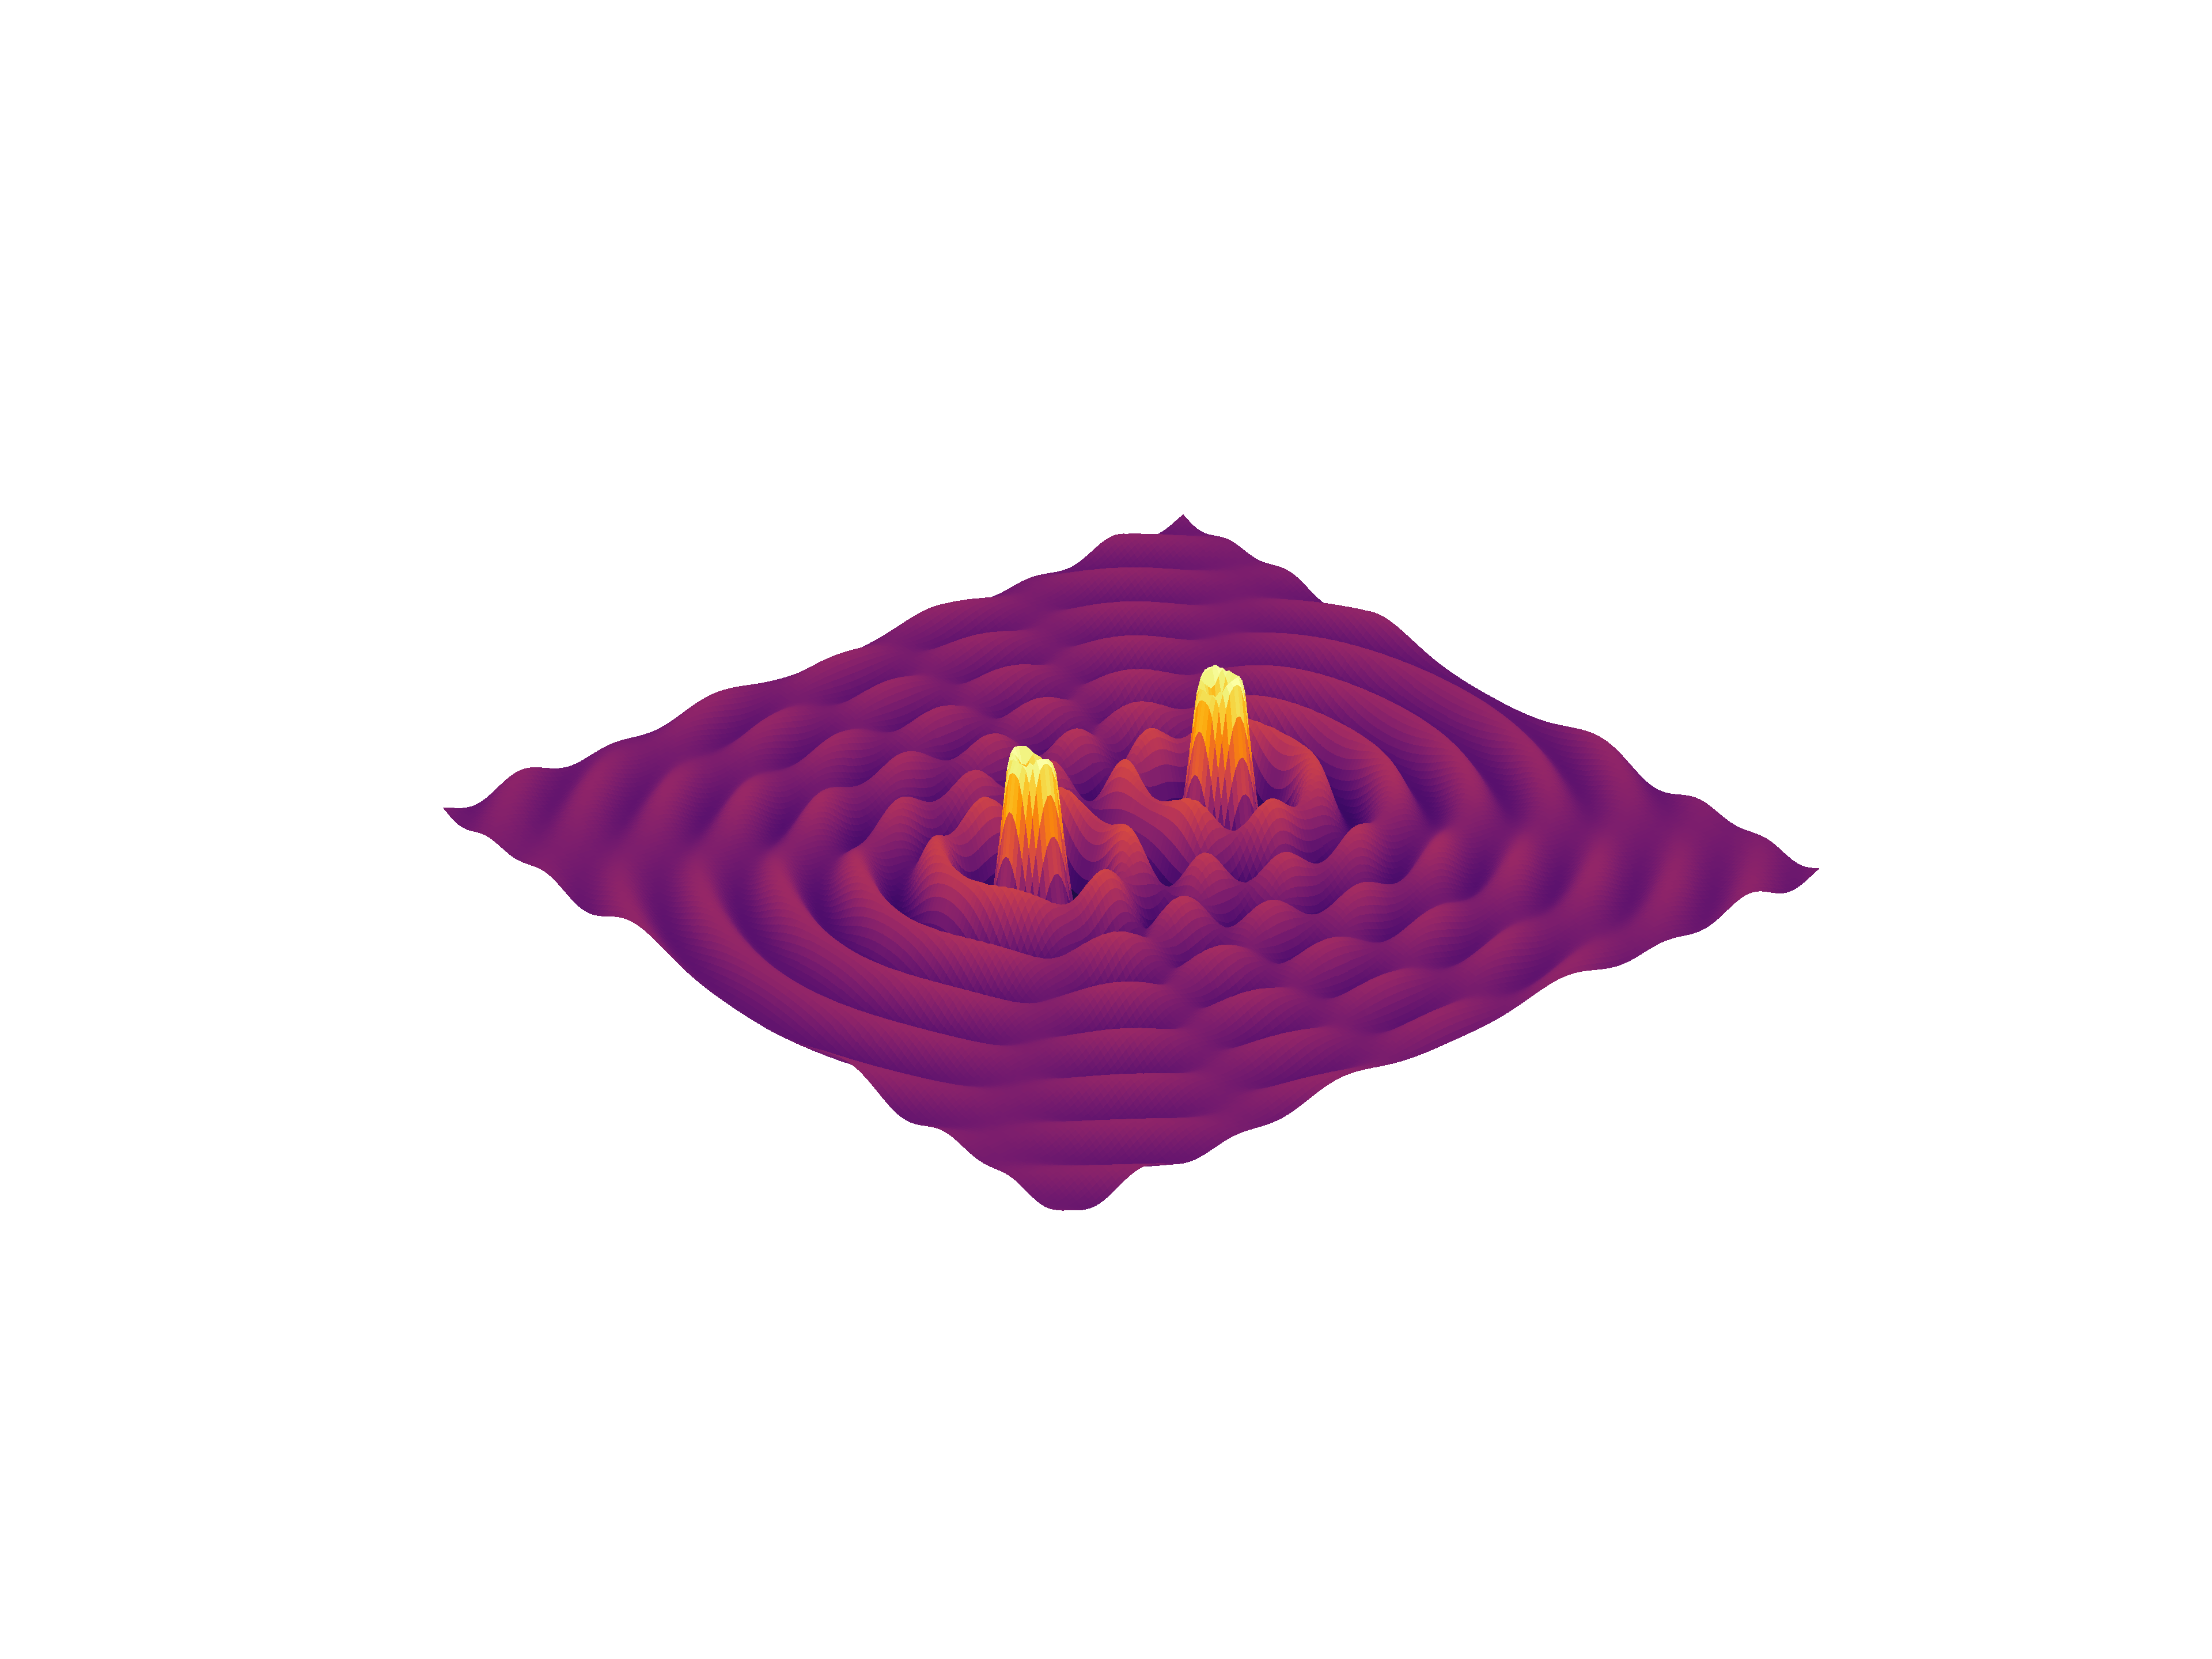
\includegraphics[scale=\myscale,scale=0.8,trim={0 2.5cm 0 3cm},clip]{figures/ondes2D-3}
\end{center}

%--------------------------------------------------------------------
\subsection{Réflexion}

\index{lumiere@lumière!reflexion@réflexion}

Un rayon lumineux se réfléchit sur un miroir selon la loi de réflexion : l'angle entre la normale et le rayon incident est égal à l'angle entre la normale et le rayon réfléchi. On renvoie aux chapitres \og{}Lancer de rayons\fg{} et \og{}Lumière\fg{} pour plus de détails.

\myfigure{0.6}{
	\tikzinput{fig-optique-01}
}

En fait, pour être plus précis, on devrait parler d'angles orientés et alors les angles incidents et réfléchis sont opposés.

\myfigure{0.6}{
	\tikzinput{fig-optique-02}
}

Considérons l'exemple suivant : on fixe un point initial et une direction à partir desquels on lance un rayon qui se réfléchit sur les quatre bords d'un rectangle. On trace alors sa trajectoire.
Ci-dessous : $1$, $2$, $10$, $100$ réflexions.
\begin{center}
	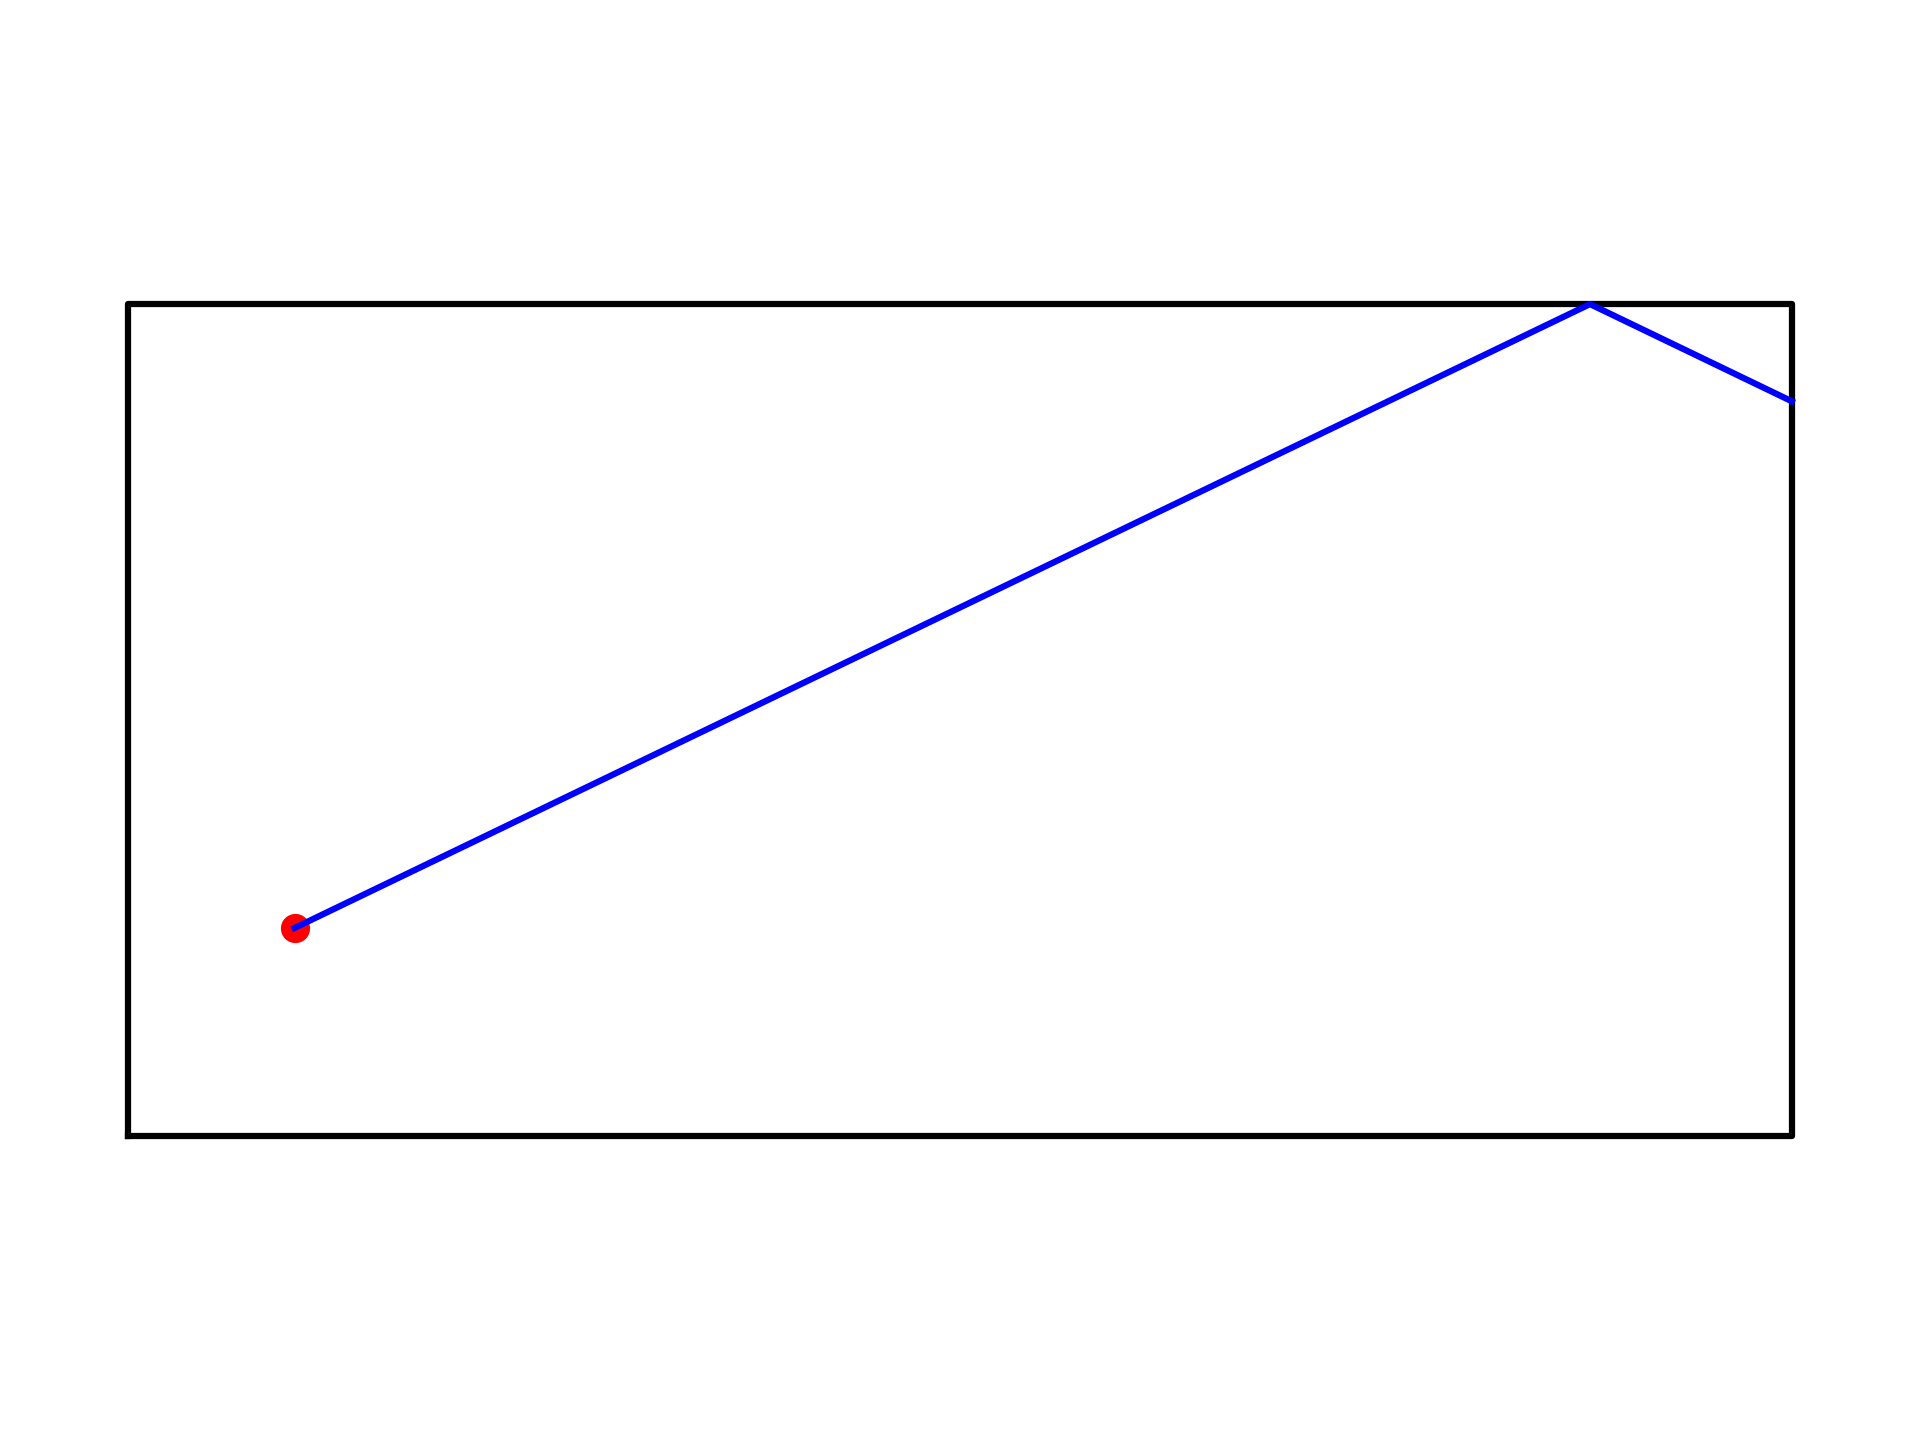
\includegraphics[scale=\myscale,scale=0.45,trim={0 1cm 0 1cm},clip]{figures/optique-1} \quad 
	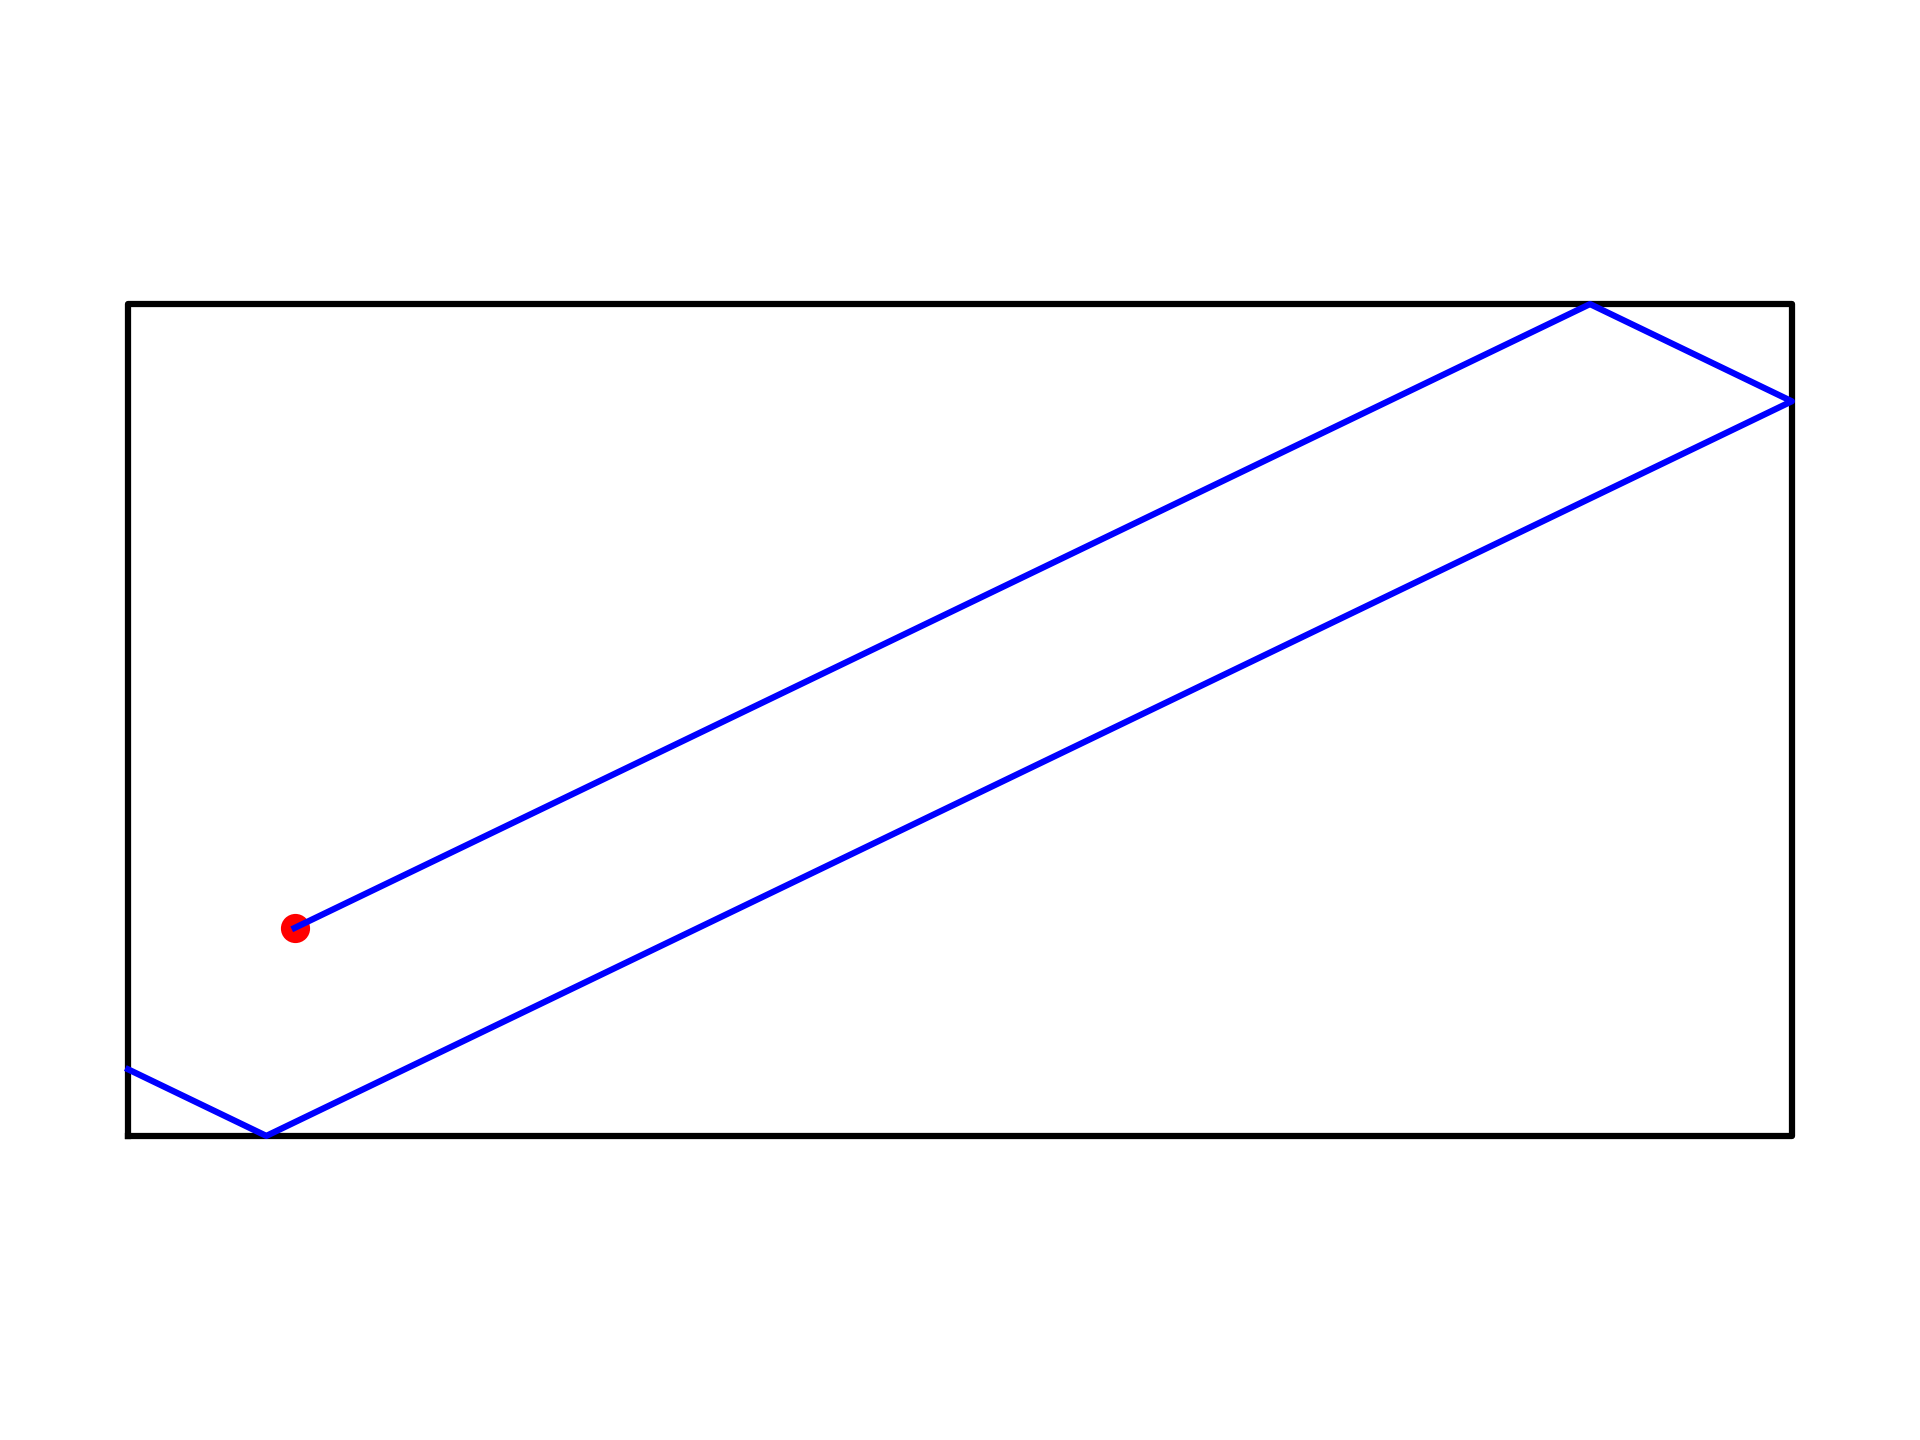
\includegraphics[scale=\myscale,scale=0.45,trim={0 1cm 0 1cm},clip]{figures/optique-2}	
	
	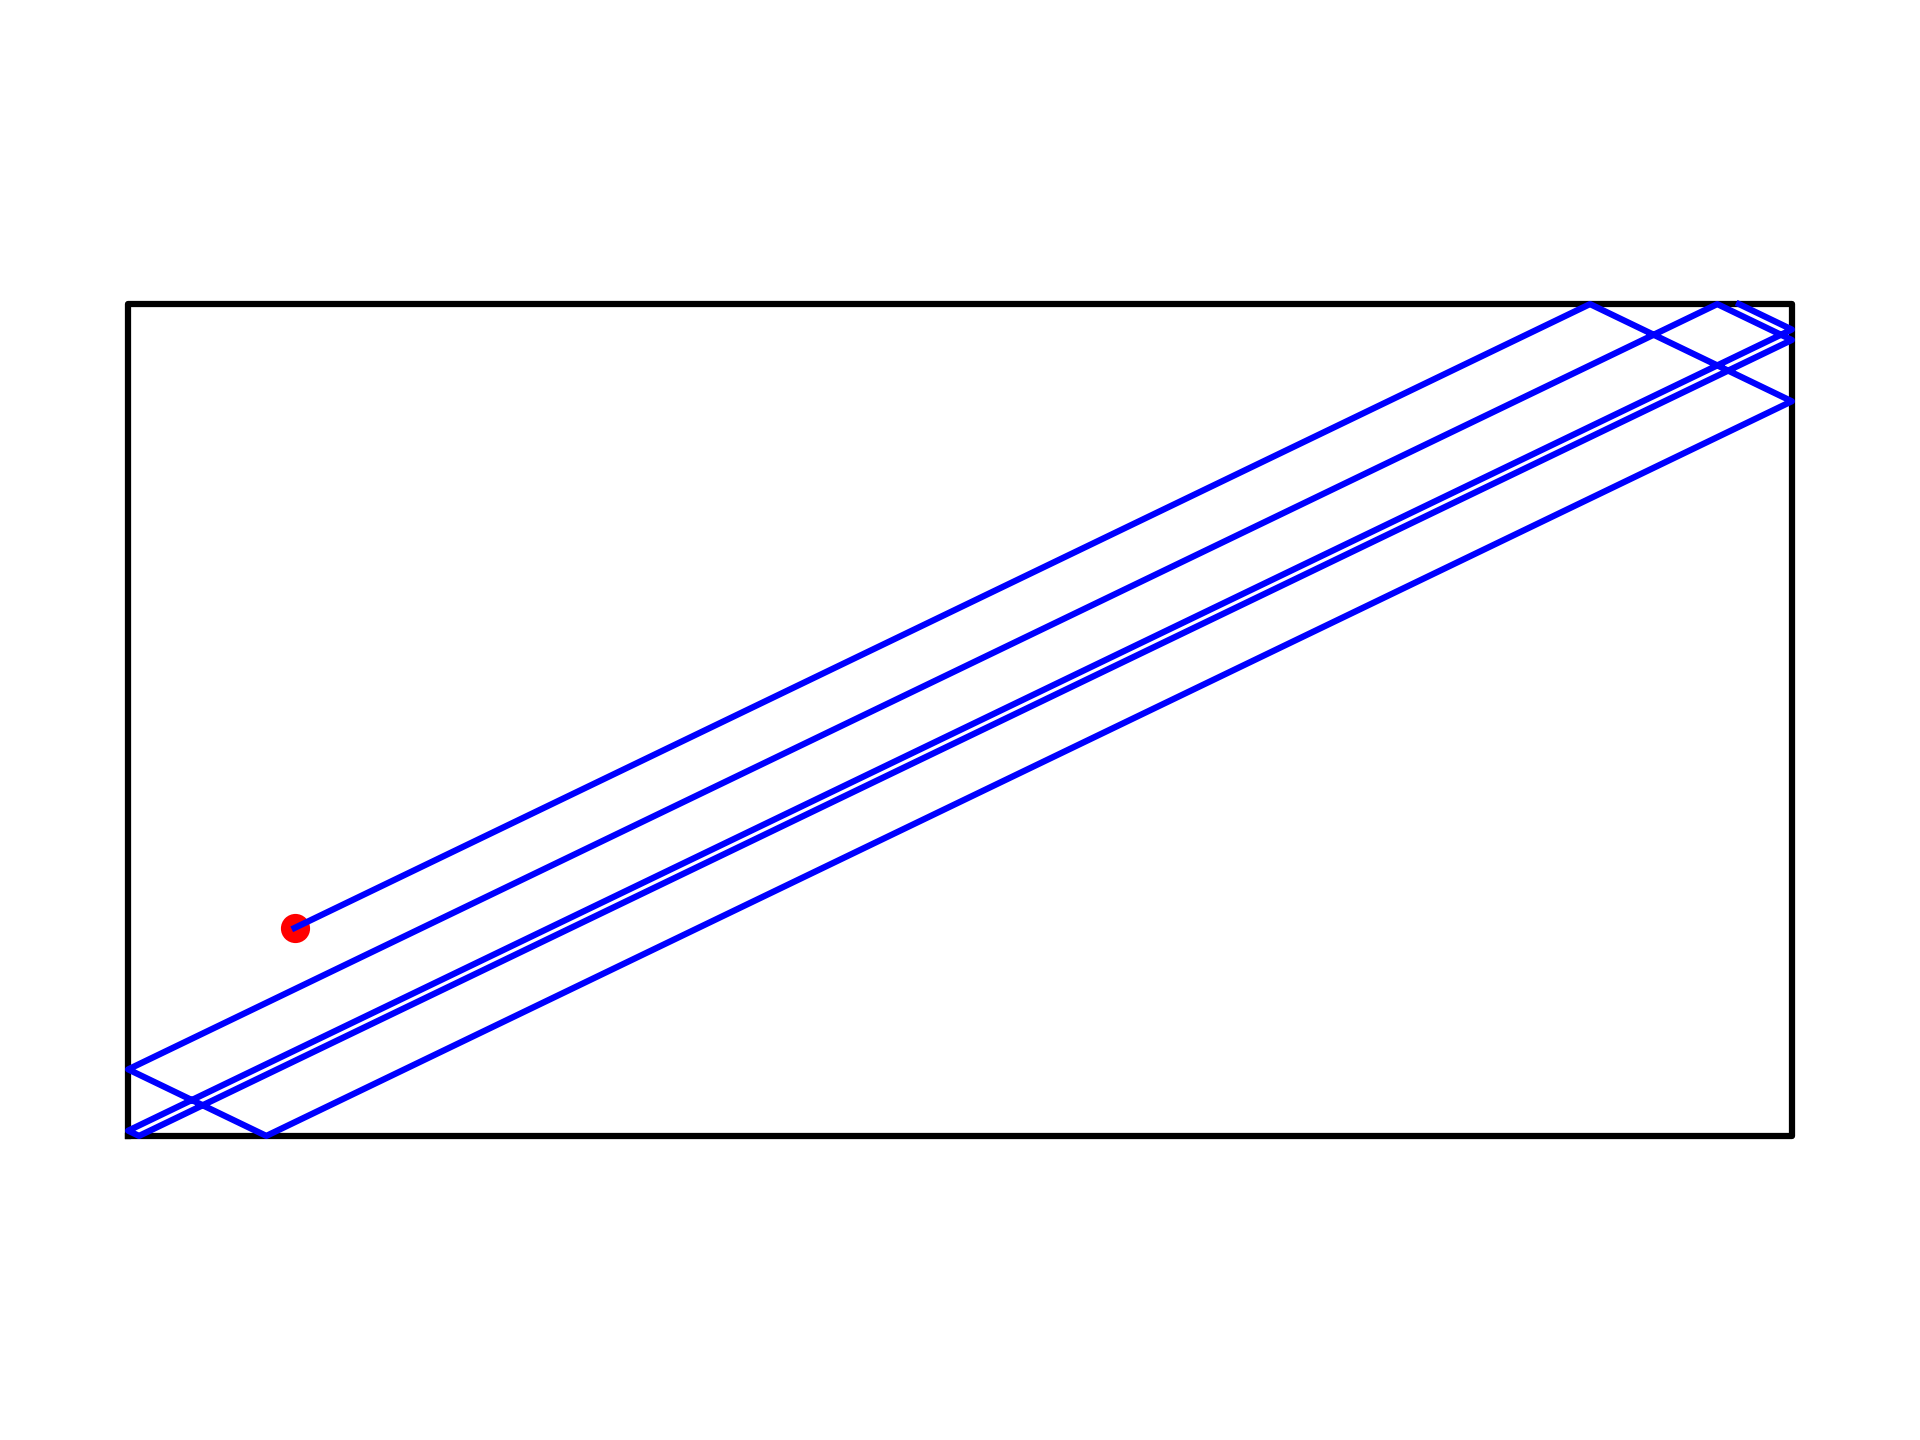
\includegraphics[scale=\myscale,scale=0.45,trim={0 1cm 0 1cm},clip]{figures/optique-3} \quad 
    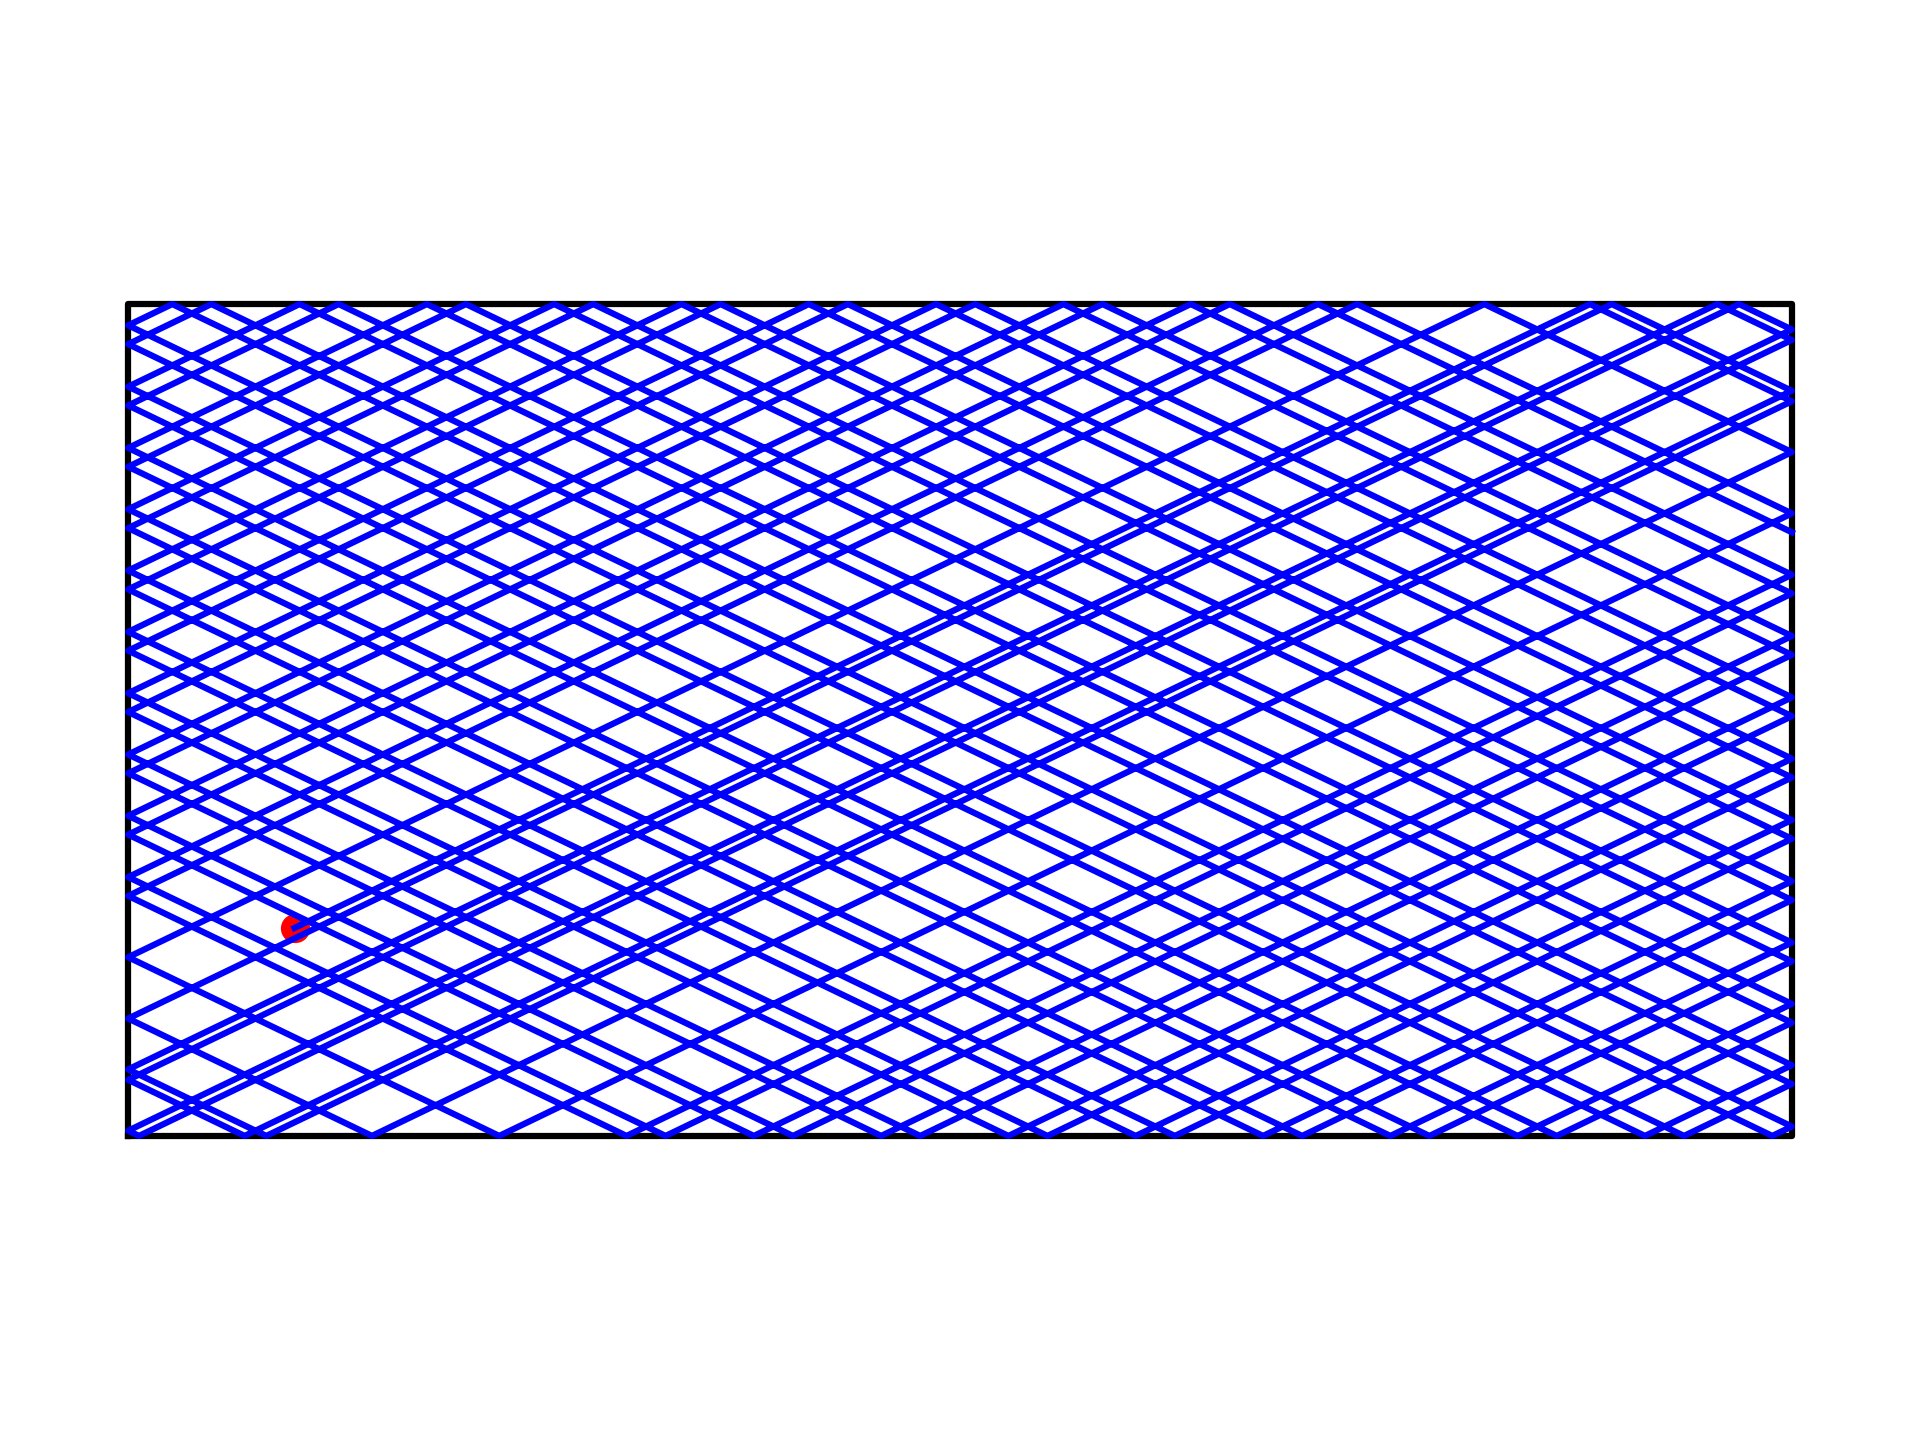
\includegraphics[scale=\myscale,scale=0.45,trim={0 1cm 0 1cm},clip]{figures/optique-4}		
\end{center}

Pour les calculs, le plus simple est de considérer le rayon paramétré par :
$$\left\{ \begin{array}{rcl}
x &=& x_0 + t \cos \theta \\
y &=& y_0 + t \sin \theta 
\end{array} \right.$$

On calcule facilement chaque paramètre $t_h$, $t_b$, $t_d$, $t_g$ qui correspond à l'intersection de chacune des faces haut/bas/droite/gauche. Par exemple, on obtient $t_h$ en résolvant l'équation $y_{\text{haut}} = y_0 + t \sin(\theta)$ (où $y_{\text{haut}}$ correspond à l'ordonnée de la face en haut). 
La face sur laquelle le rayon se réfléchit correspond au paramètre $t>0$ le plus petit parmi $t_h$, $t_b$, $t_d$, $t_g$.
Si par exemple le rayon se réfléchit sur la face haute alors on repart du point de cette face mais cette fois avec un angle $-\theta$.



%--------------------------------------------------------------------
\subsection{Réfraction}

\index{lumiere@lumière!refraction@réfraction}

Lorsque un rayon lumineux change de milieu, par exemple passe de l'air à l'eau, la trajectoire du rayon est modifiée : c'est un phénomène de réfraction.

La \defi{loi de Snell-Descartes}\index{loi!de Snell-Descartes} relie l'angle entre le rayon incident avec la normale et le rayon réfracté et la normale :
\mybox{$n_1 \sin \theta_1 = n_2 \sin \theta_2$}

$n_1$ et $n_2$ et sont les indices des milieux correspondants, par exemple l'indice de l'air est environ $n_{\text{air}} \simeq 1$ et celui de l'eau est $n_{\text{eau}} \simeq 1.33$.

\myfigure{0.7}{
	\tikzinput{fig-optique-03}
}

 
\begin{center}
	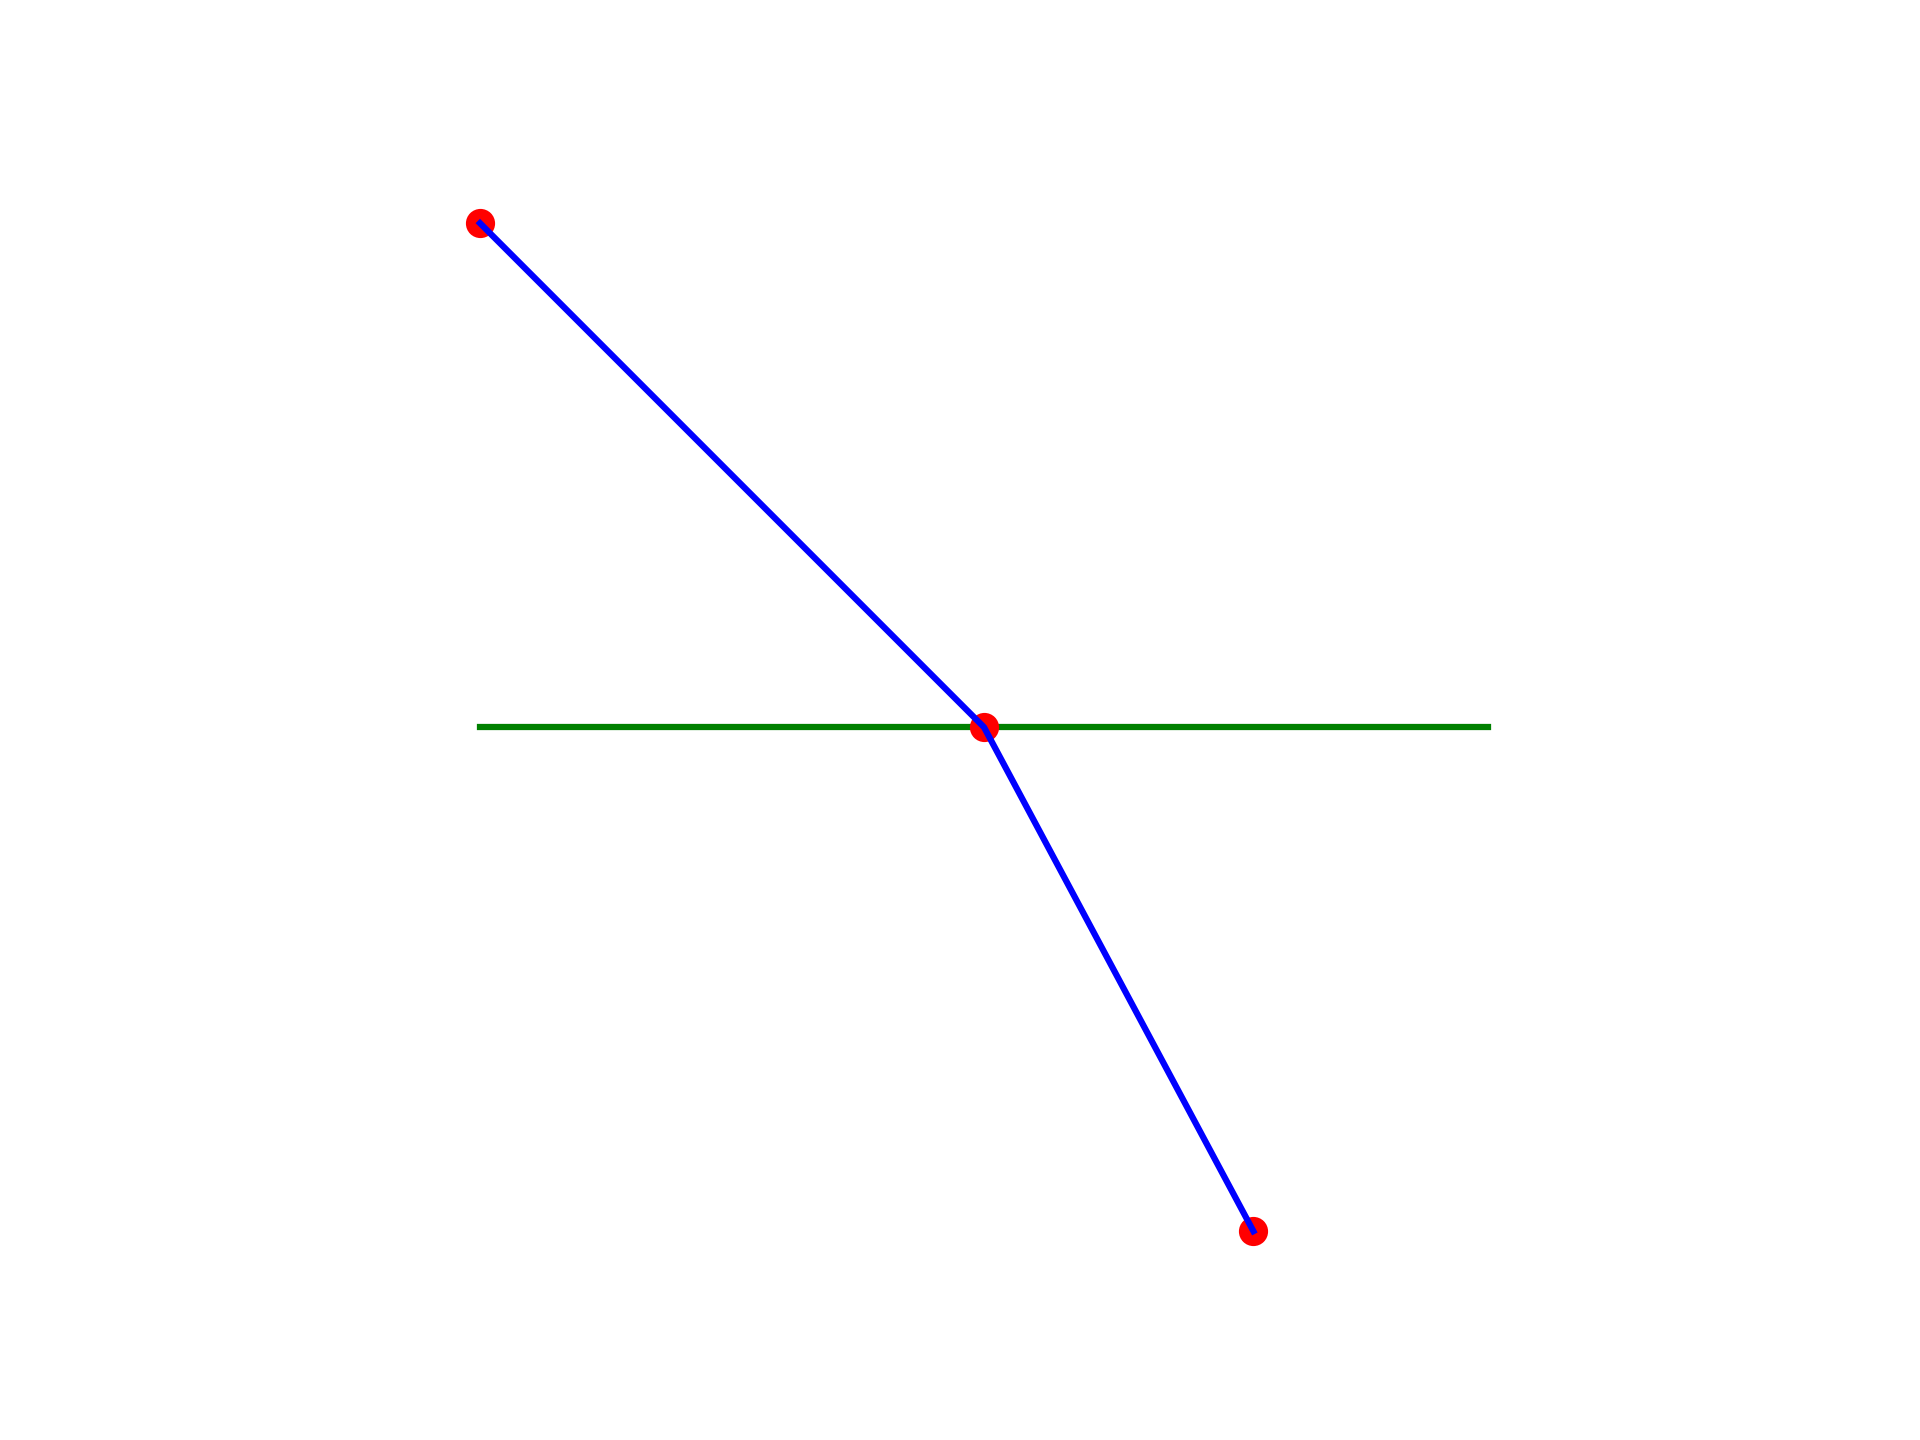
\includegraphics[scale=\myscale,scale=0.5]{figures/refraction-1} \quad 
	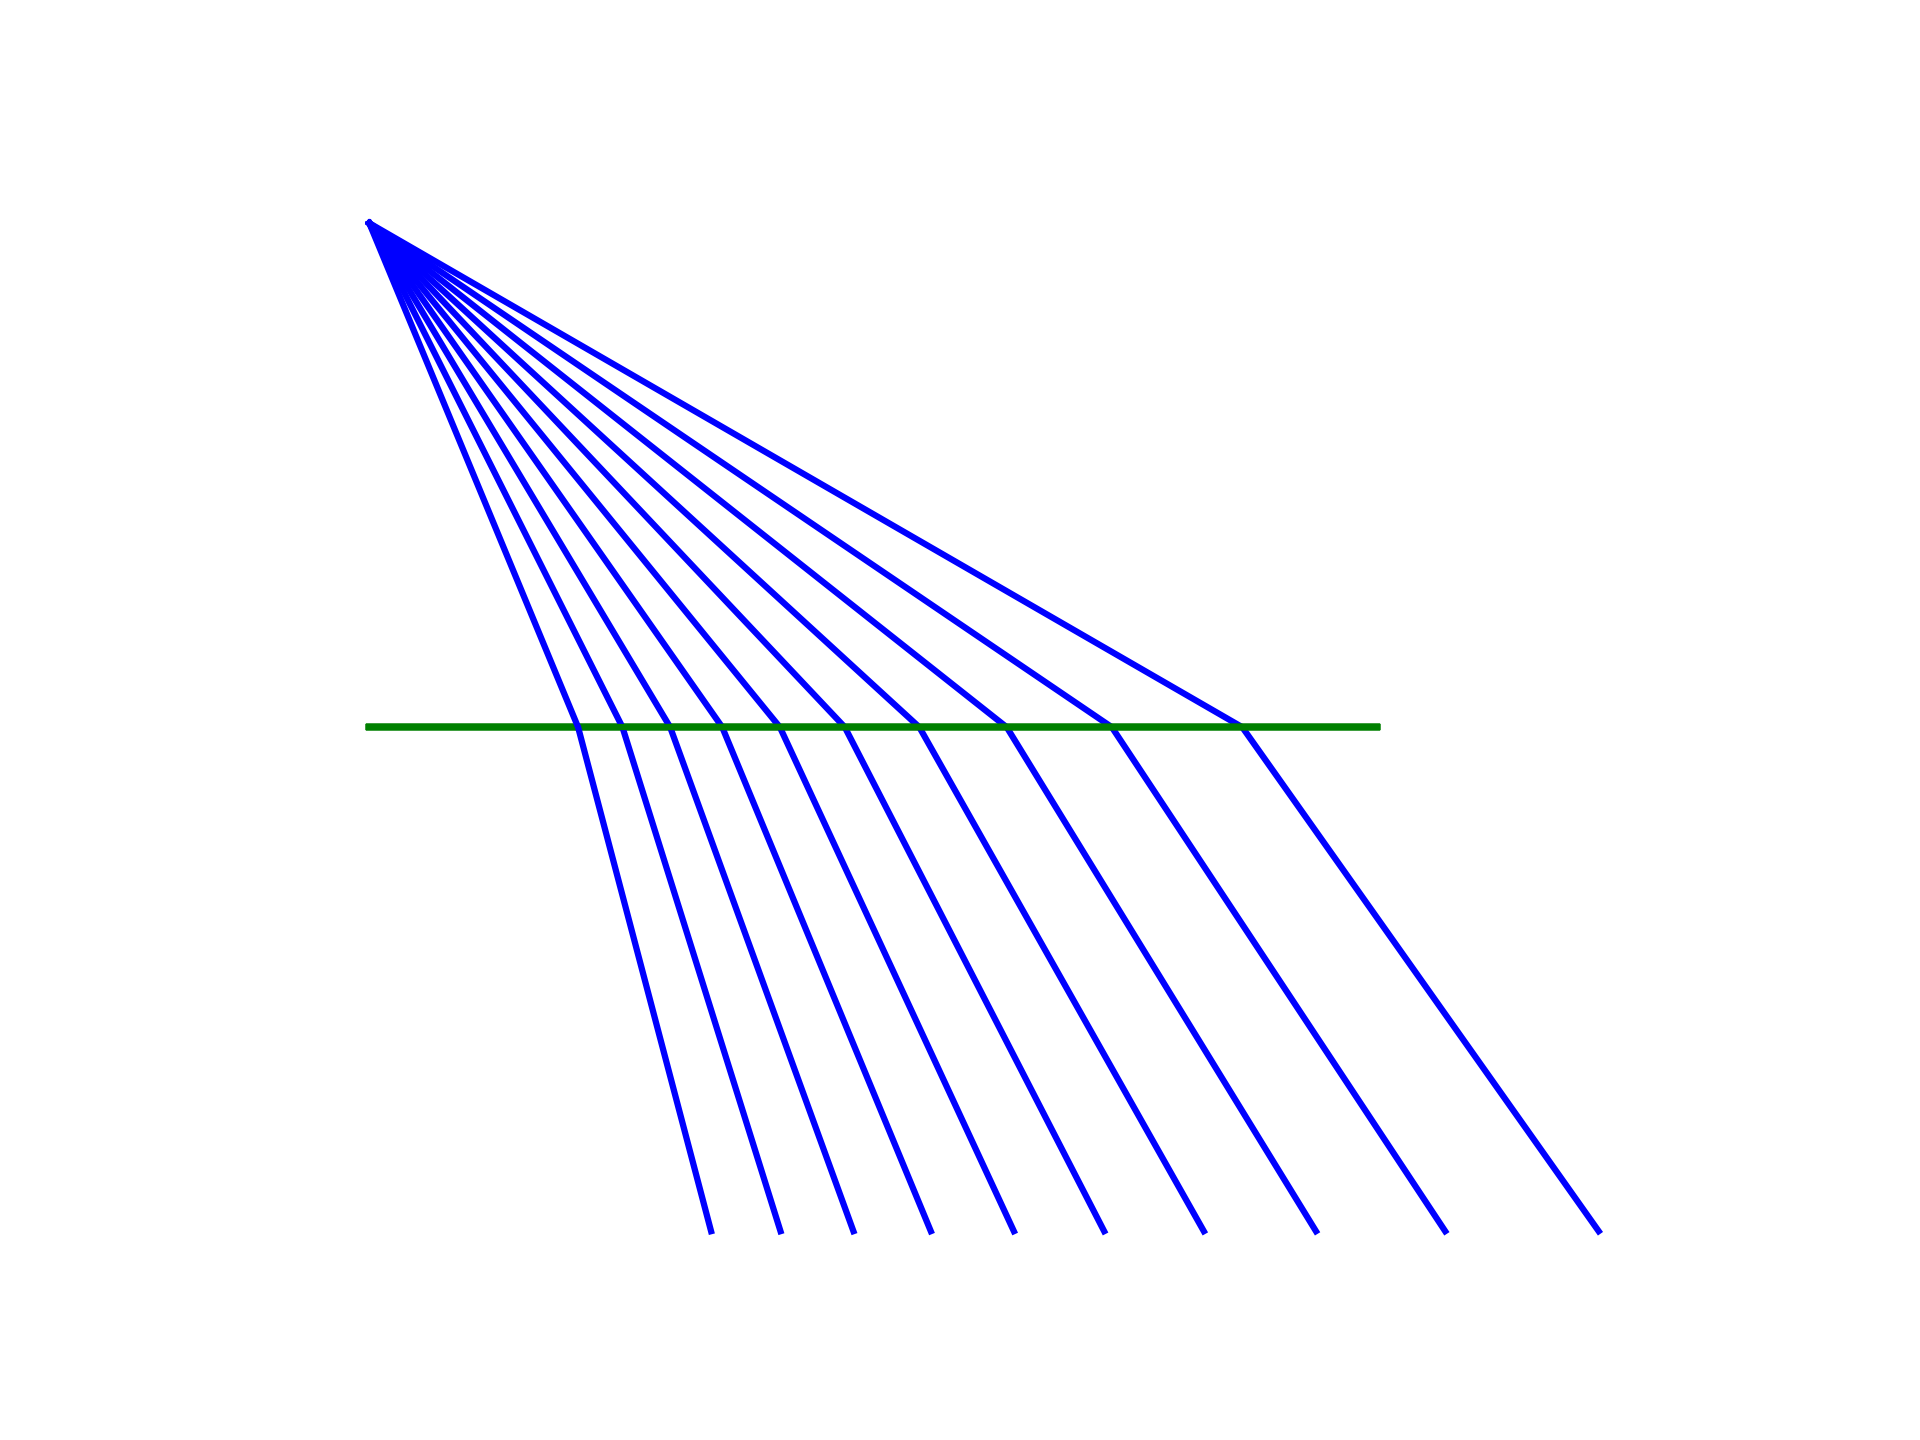
\includegraphics[scale=\myscale,scale=0.5]{figures/refraction-2}			
\end{center}


L'indice du verre est environ $n_{\text{verre}} \simeq 1.5$. Mais en fait l'indice précis dépend de la longueur d'onde du rayon lumineux. Un rayon de lumière blanche est la superposition de rayons lumineux de différentes longueurs d'onde (du violet de longueur d'onde démarrant à $380$ nanomètres au rouge terminant vers $\SI{780}{\nano\meter}$).
Comme l'indice du verre dépend de la longueur d'onde, le rayon de lumière blanche va se séparer en différents rayons colorés en traversant la surface du verre. L'expérience de Newton avec un prisme de verre met ainsi en évidence le spectre de la lumière blanche.

Une formule approchée, dite de Cauchy, pour l'indice du verre est
$$n_{\text{verre}}(\lambda) = 1.4580 + \frac{0.0354}{\lambda^2}$$
où $\lambda$ est la longueur l'onde du rayon incident exprimée en micromètre (donc variant de $0.380$ à $0.780$).

C'est un bon exercice de programmation de simuler cette expérience fondamentale.


\begin{center}
	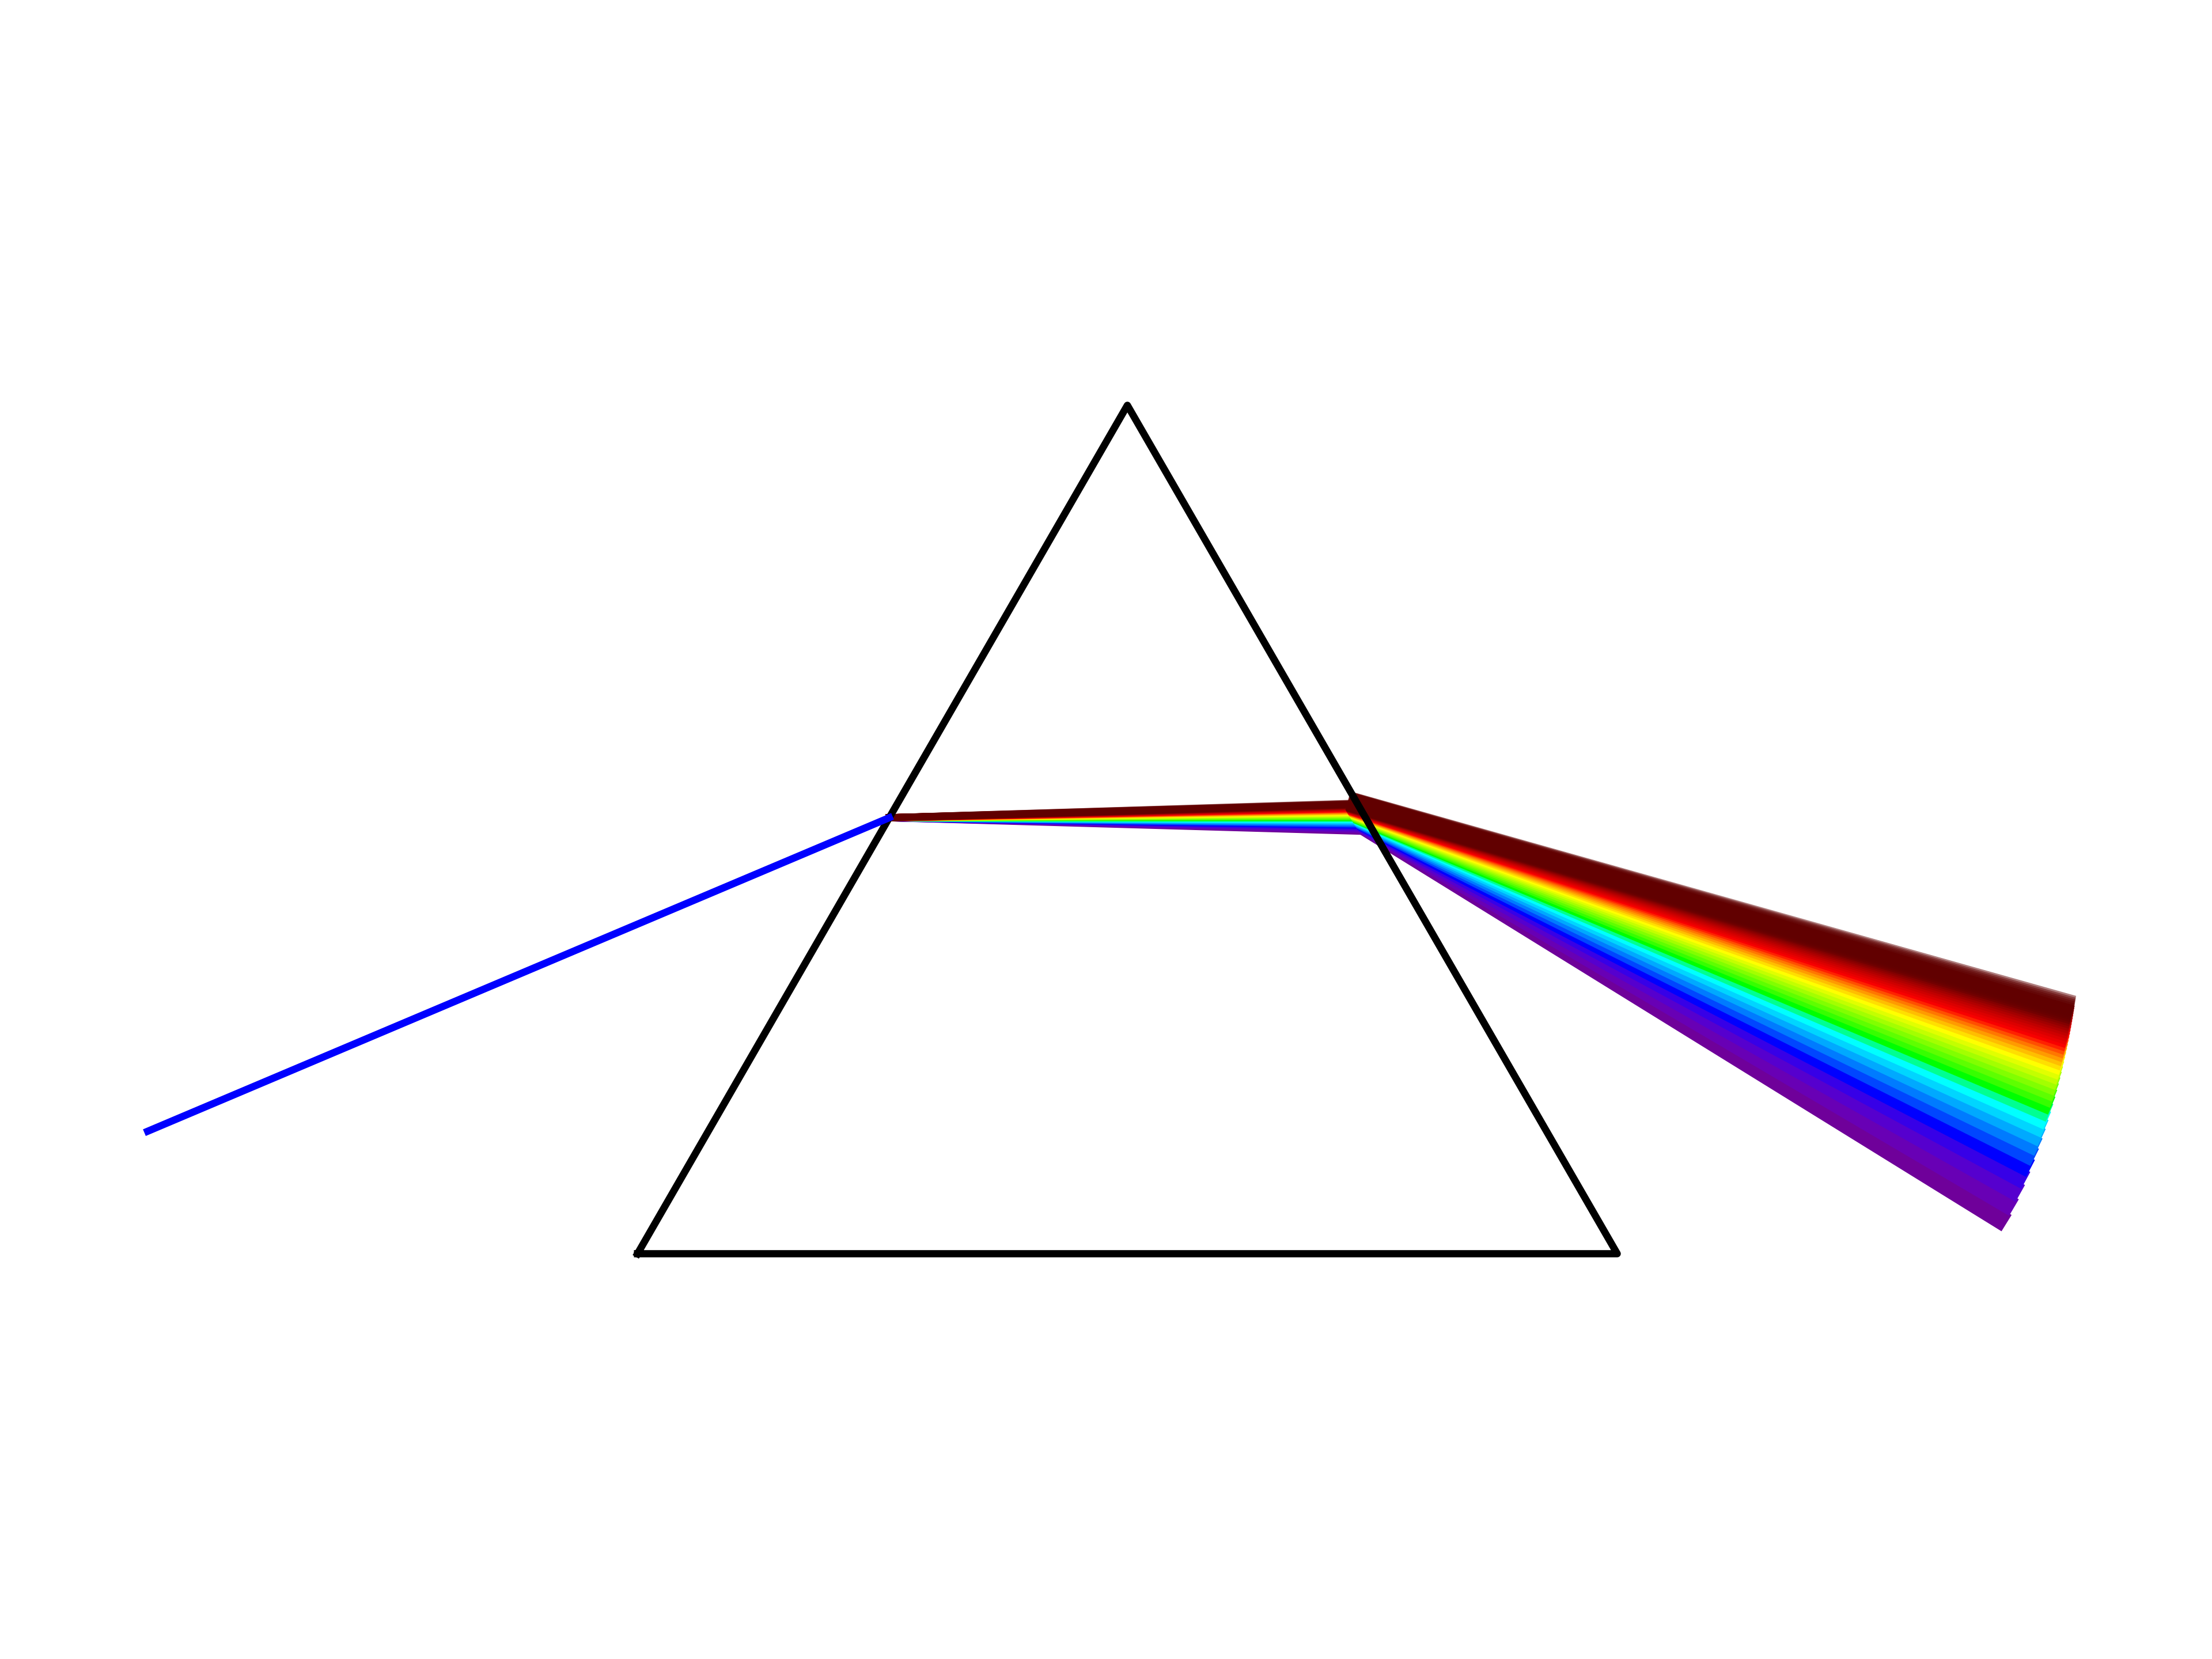
\includegraphics[scale=\myscale,scale=1,trim={0 2cm 0 3cm},clip]{figures/prisme}			
\end{center}




%%%%%%%%%%%%%%%%%%%%%%%%%%%%%%%%%%%%%%%%%%%%%%%%%%%%%%%%%%%%%%%%%%%%%
\section{Liquide et gaz}

La modélisation des fluides est extrêmement complexe.
La mécanique des liquides et des gaz est régie par des lois approximant le comportement  fluide en supposant des propriétés simplificatrices (par exemple fluide sans viscosité ou bien incompressible...). Même avec ces hypothèses, les équations qui régissent le comportement sont des équations différentielles (plus précisément des équations aux dérivées partielles) dont on ne sait en général pas calculer des solutions explicites.
Les équations simples (fluide sans viscosité) sont les équations d'Euler, le cas général est régi par les équations de Navier-Stokes (dont personne ne connaît de solution générale et qui font l'objet de recherches actives).

Nous allons modéliser le déplacement d'un fluide incompressible dans un tube lorsqu'il rencontre un obstacle (ici un disque).
Cette section est basée sur l'article \emph{Create your own lattice Boltzmann simulation} de Philip Mocz.
 
\begin{center}	
	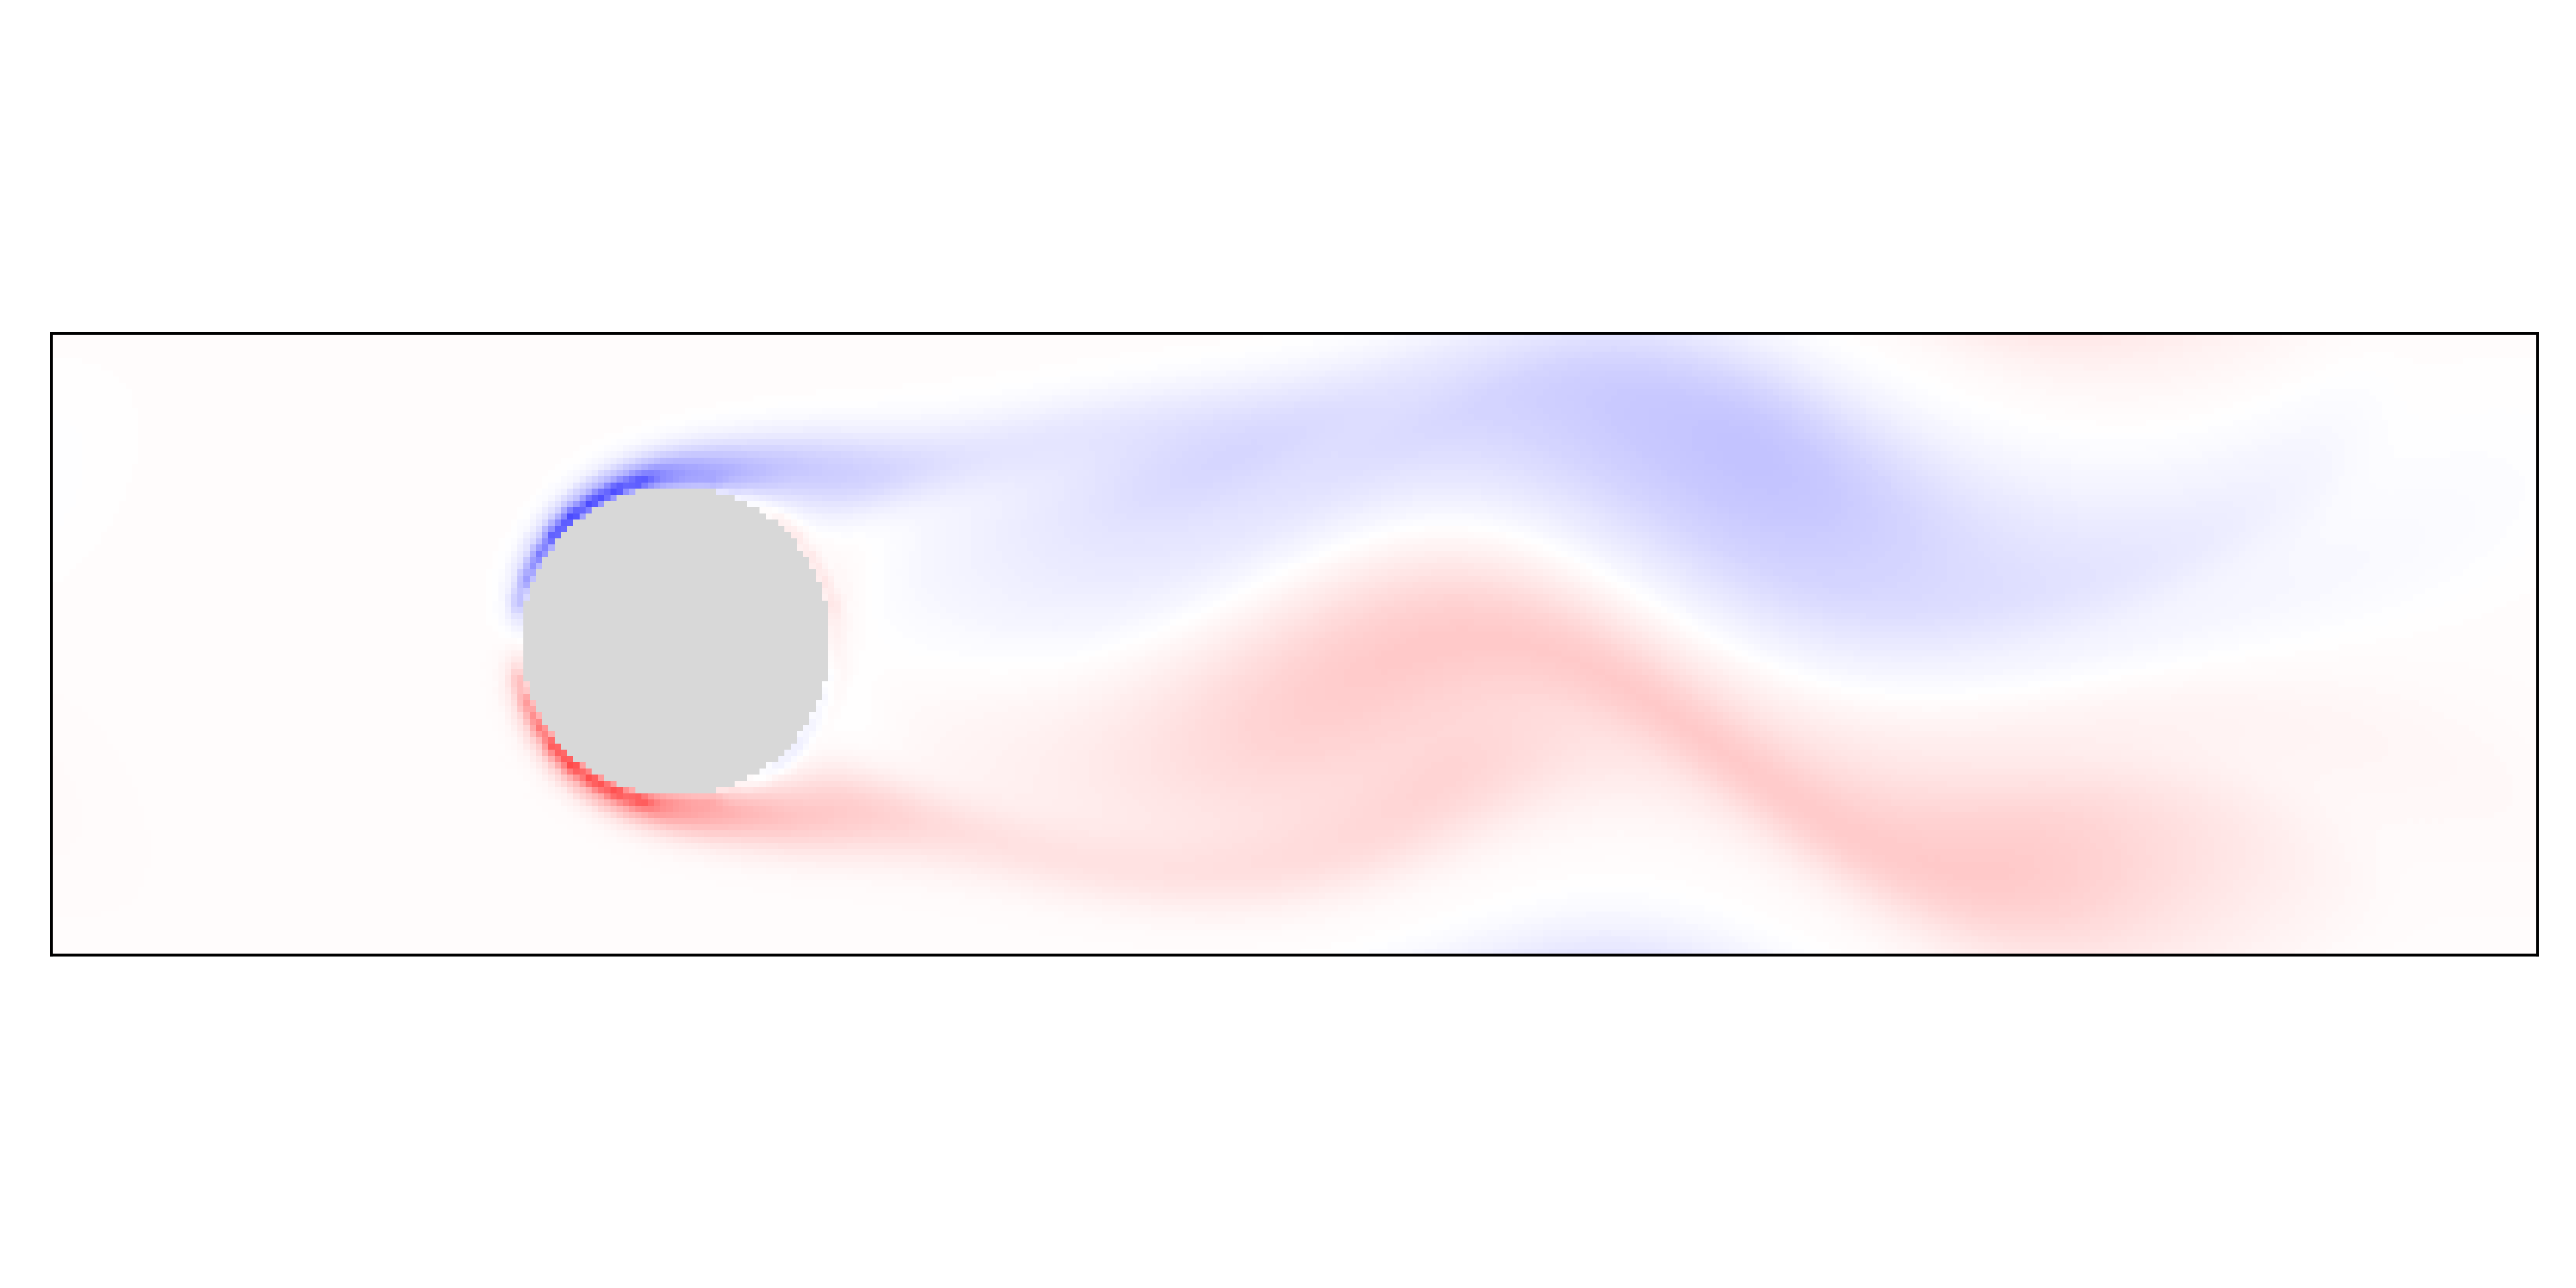
\includegraphics[scale=\myscale,scale=0.6,trim={0 2cm 0 3cm},clip]{figures/fluide-vortex-3000}			
\end{center}

%--------------------------------------------------------------------
\subsection{Réseau de Boltzmann}

Commençons par décrire le comportement à l'équilibre d'un liquide ou d'un gaz par une modélisation microscopique d'une seule particule.
Même si le fluide est globalement à l'équilibre chaque particule peut se déplacer de façon aléatoire.
Nous modélisons le lieu d'évolution par une grille rectangulaire de taille $N_x \times N_y$ dans laquelle on a placé un obstacle (ici un disque).

\myfigure{0.9}{
	\tikzinput{fig-fluide-01}
}


Dans un premier temps on considère que dans chaque case $(x,y)$ on place une particule ; à l'instant $t + \dd t$ suivant cette particule peut se déplacer sur l'une des 8 cases voisines ou bien rester à sa place. 

\myfigure{0.7}{
	\tikzinput{fig-fluide-02}
}


Comme on ne sait pas quel va être le comportement de cette particule et qu'on veut considérer toutes les possibilités on remplace cette grosse particule dans la case $(x,y)$ par $36$ mini-particules.
Ces $36$ mini-particules représentent toutes les possibilités de déplacement en tenant compte des probabilités : $16$ mini-particules resteront immobiles, $4$ mini-particules iront vers la case de droite, $4$ vers la case de gauche, \ldots, $1$ seule mini-particule sur les $36$ ira sur la case en haut à droite,\ldots{}

\myfigure{0.7}{
	\tikzinput{fig-fluide-03}
}




On associe donc à chaque mini-particule en $(x,y)$ un vecteur vitesse $\vec{v_i}$ 
parmi $\vec{v_0} = (0,0)$ (la mini-particule reste immobile), $\vec{v_1} = (0,1)$ (la mini-particule va monter d'une case), \ldots, $\vec {v_8} = (-1,1)$.

\myfigure{0.7}{
	\tikzinput{fig-fluide-04}
}

Ainsi l'ensemble des mini-particules est modélisé par une fonction $F(x,y,i)$
qui compte le nombre de particules dans la case $(x,y)$ ayant pour vecteur vitesse  $\vec{v_i}$. Par exemple $F(x,y,1)$ compte le nombre de mini-particules sur la case $(x,y)$ qui à l'instant suivant se déplaceront vers la case $(x,y+1)$.



%--------------------------------------------------------------------
\subsection{Mouvement}

Comment modéliser le déplacement ? C'est tout simple : chaque mini-particule se déplace en suivant son vecteur vitesse. Ainsi les mini-particules sur la case $(x,y)$ avec le vecteur $\vec{v_i}$ se déplacent à l'instant suivant vers la case $(x,y) + \vec{v_i}$. En plus, par inertie, elles conservent leur vecteur vitesse $\vec{v_i}$.

\myfigure{0.7}{
	\tikzinput{fig-fluide-05}
}

Sur une case $(x,y)$ des mini-particules peuvent arriver de plusieurs directions, mais si on impose en plus le vecteur vitesse alors les mini-particules ne proviennent que d'une seule case. D'où la formule :
$$F(x + v_{x,i}, y + v_{y,i}, i) = F(x, y, i)$$
où $\vec {v_i} = (v_{x,i}, v_{y,i})$.


%--------------------------------------------------------------------
\subsection{Flux vers la droite}

Pour l'instant depuis une case les mini-particules se déplacent vers la droite ou vers la gauche de manière équiprobable. Si on veut modéliser un flux vers la droite (par exemple l'eau d'une rivière qui s'écoule de la gauche vers la droite, ou bien l'action d'un ventilateur ou d'une turbine) il suffit d'ajouter des mini-particules ayant le vecteur vitesse $\vec{v_3} = (1,0)$.
Par exemple on y place $12$ mini-particules au lieu des $4$ de l'état d'équilibre.

\myfigure{0.7}{
	\tikzinput{fig-fluide-06}
}

Pour éviter un modèle trop \og{}lisse\fg{} on perturbe aléatoirement l'initialisation : on ajoute au hasard, ici où là, une mini-particule à l'état $(x,y,i)$.


%--------------------------------------------------------------------
\subsection{Obstacle}

Que fait la particule lorsqu'elle rencontre un obstacle ? Elle repart simplement en sens inverse. C'est une approximation grossière dans laquelle on considère que nos mini-particules arrivent perpendiculairement au bord.
Plus en détails : si une particule $(x,y)$ de vecteur $\vec{v_i}$ devait se retrouver à la prochaine itération dans l'obstacle, au lieu de se retrouver en $(x,y) + \vec{v_i}$, on la conserve en $(x,y)$ mais avec le vecteur $-\vec{v_i}$.

\myfigure{0.8}{
	\tikzinput{fig-fluide-07}
}


%--------------------------------------------------------------------
\subsection{Densité et vitesse}

La \emph{densité} $\rho$ en $(x,y)$ est le nombre de mini-particules dans la case $(x,y)$, elle s'obtient en comptant les mini-particules en $(x,y)$ quel que soit leur vecteur vitesse :
$$\rho(x,y) = F(x,y,0) + F(x,y,1) + \cdots + F(x,y,8).$$

Lors de l'initialisation il est préférable de supposer que la densité vaut $1$ en tout $(x,y)$ quitte à faire une étape de renormalisation.
Par exemple, voici une case $(x,y)$ de densité $1$ qui correspond à un état d'équilibre (sans flux) : une mini-particule correspond ici à $1/36$ d'une particule.

\myfigure{0.7}{
	\tikzinput{fig-fluide-08}
}

Par contre au fil du temps la densité va évoluer et ne vaut plus $1$ partout.

\medskip

Une autre valeur physique importante est le \emph{vecteur vitesse} $\vec{u}(x,y)$ en $(x,y)$. On calcule ce vecteur vitesse en le décomposant sous la forme (vitesse horizontale, vitesse verticale) :  $\vec{u} = (u_x, u_y)$.
La \emph{vitesse horizontale} est le nombre de mini-particules allant vers la droite moins le nombre de mini-particules allant vers la gauche divisé par la densité :
$$u_x(x,y) = \frac{1}{\rho(x,y)} \big(F(x,y,2) + F(x,y,3) + F(x,y,4) - F(x,y,6) - F(x,y,7) - F(x,y,8)\big).$$
La \emph{vitesse verticale} est le nombre de mini-particules montantes moins le nombre de mini-particules descendantes (divisé par le nombre total de mini-particules) :
$$u_x(x,y) = \frac{1}{\rho(x,y)} \big(F(x,y,1) + F(x,y,2) - F(x,y,4) - F(x,y,5) - F(x,y,6) + F(x,y,8)\big).$$ 


%--------------------------------------------------------------------
\subsection{Collision et fonction d'équilibre}

Voici les trois étapes lors de chaque itération correspondant à un intervalle de temps élémentaire $\dd t$ :
\begin{enumerate}
	\item \emph{Mouvement :} chaque mini-particule se déplace suivant son vecteur vitesse $\vec{v_i}$ : $F(x + v_{x,i}, y + v_{y,i}, i) = F(x, y, i)$.
	
	\item \emph{Obstacle :} les mini-particules qui rencontrent l'obstacle font demi-tour, pour elles $\vec{v_i}$ devient $-\vec{v_i}$.
	
	\item \emph{Collision :}
	on modifie la densité $F$ afin de tenir compte des collisions entre particules, cela se fait à l'aide d'une fonction d'équilibre $F_{\text{eq}}$ et on remplace $F$ par $F - \frac{1}{\tau} (F-F_{\text{eq}})$.
\end{enumerate}

Détaillons cette dernière étape.
Tout d'abord la fonction d'équilibre est issue de la physique et des équations de Navier-Stokes :
$$F_{\text{eq}} (x,y,i) = w_i \, \rho(x,y) \left(1 + 3 \vec{u} \cdot \vec{v_i}  +  \frac92(\vec{u} \cdot \vec{v_i})^2 - \frac32 \| \vec u \| ^2 \right).$$
C'est-à-dire :
$$F_{\text{eq}} (x,y,i) = w_i \, \rho(x,y) \left(1 + 3( u_x v_{x,i} + u_y v_{y,i}) + \frac92(u_x v_{x,i} + u_y v_{y,i})^2 - \frac32 (u_x^2 + u_y^2) \right).$$
On a abrégé $u_x(x,y)$, $v_{x,i}(x,y)$\ldots en $u_x$, $v_{x_i}$\ldots

Les $w_i$ ($i=0,\ldots,8$) sont les poids associés à la position d'équilibre statique $w_0 = \frac{16}{36}$, $w_1 = \frac{4}{36}$, \ldots 

\myfigure{0.7}{
	\tikzinput{fig-fluide-09}
}

Pour tenir compte des collisions entre particules on mesure la différence entre l'état actuel et l'état à l'équilibre, que l'on pondère par un coefficient $\frac{1}{\tau}$ (où $\tau$ est le temps de collision, par exemple $\tau=0.6$). 
On remplace $F(x,y,i)$ par $F(x,y,i) - \frac1\tau \big(F(x,y,i)-F_{\text{eq}}(x,y,i)\big)$,
autrement dit on définirait par récurrence $F_{n+1}(x,y,i) = F_n(x,y,i) - \frac1\tau \big(F_n(x,y,i)-F_{\text{eq}}(x,y,i)\big)$.
	
	
%--------------------------------------------------------------------
\subsection{Résultats}

Voici quelques images illustrant les résultats. 
Ci-dessous la mesure de la vitesse $\| \vec{u}(x,y) \|$ des particules après 100 itérations (en haut) et 500 (en bas).
On remarque que les particules sont plus rapides en-dessous et au-dessus de l'obstacle\couleurnb{ (en rouge)}{} et plus lentes avant et après l'obstacle\couleurnb{ (en bleu)}{}. Cela reflète bien que les particules sont bloquées par l'obstacle et aussi que le flux doit accélérer au niveau de l'obstacle car le passage y est moins large.
\begin{center}
	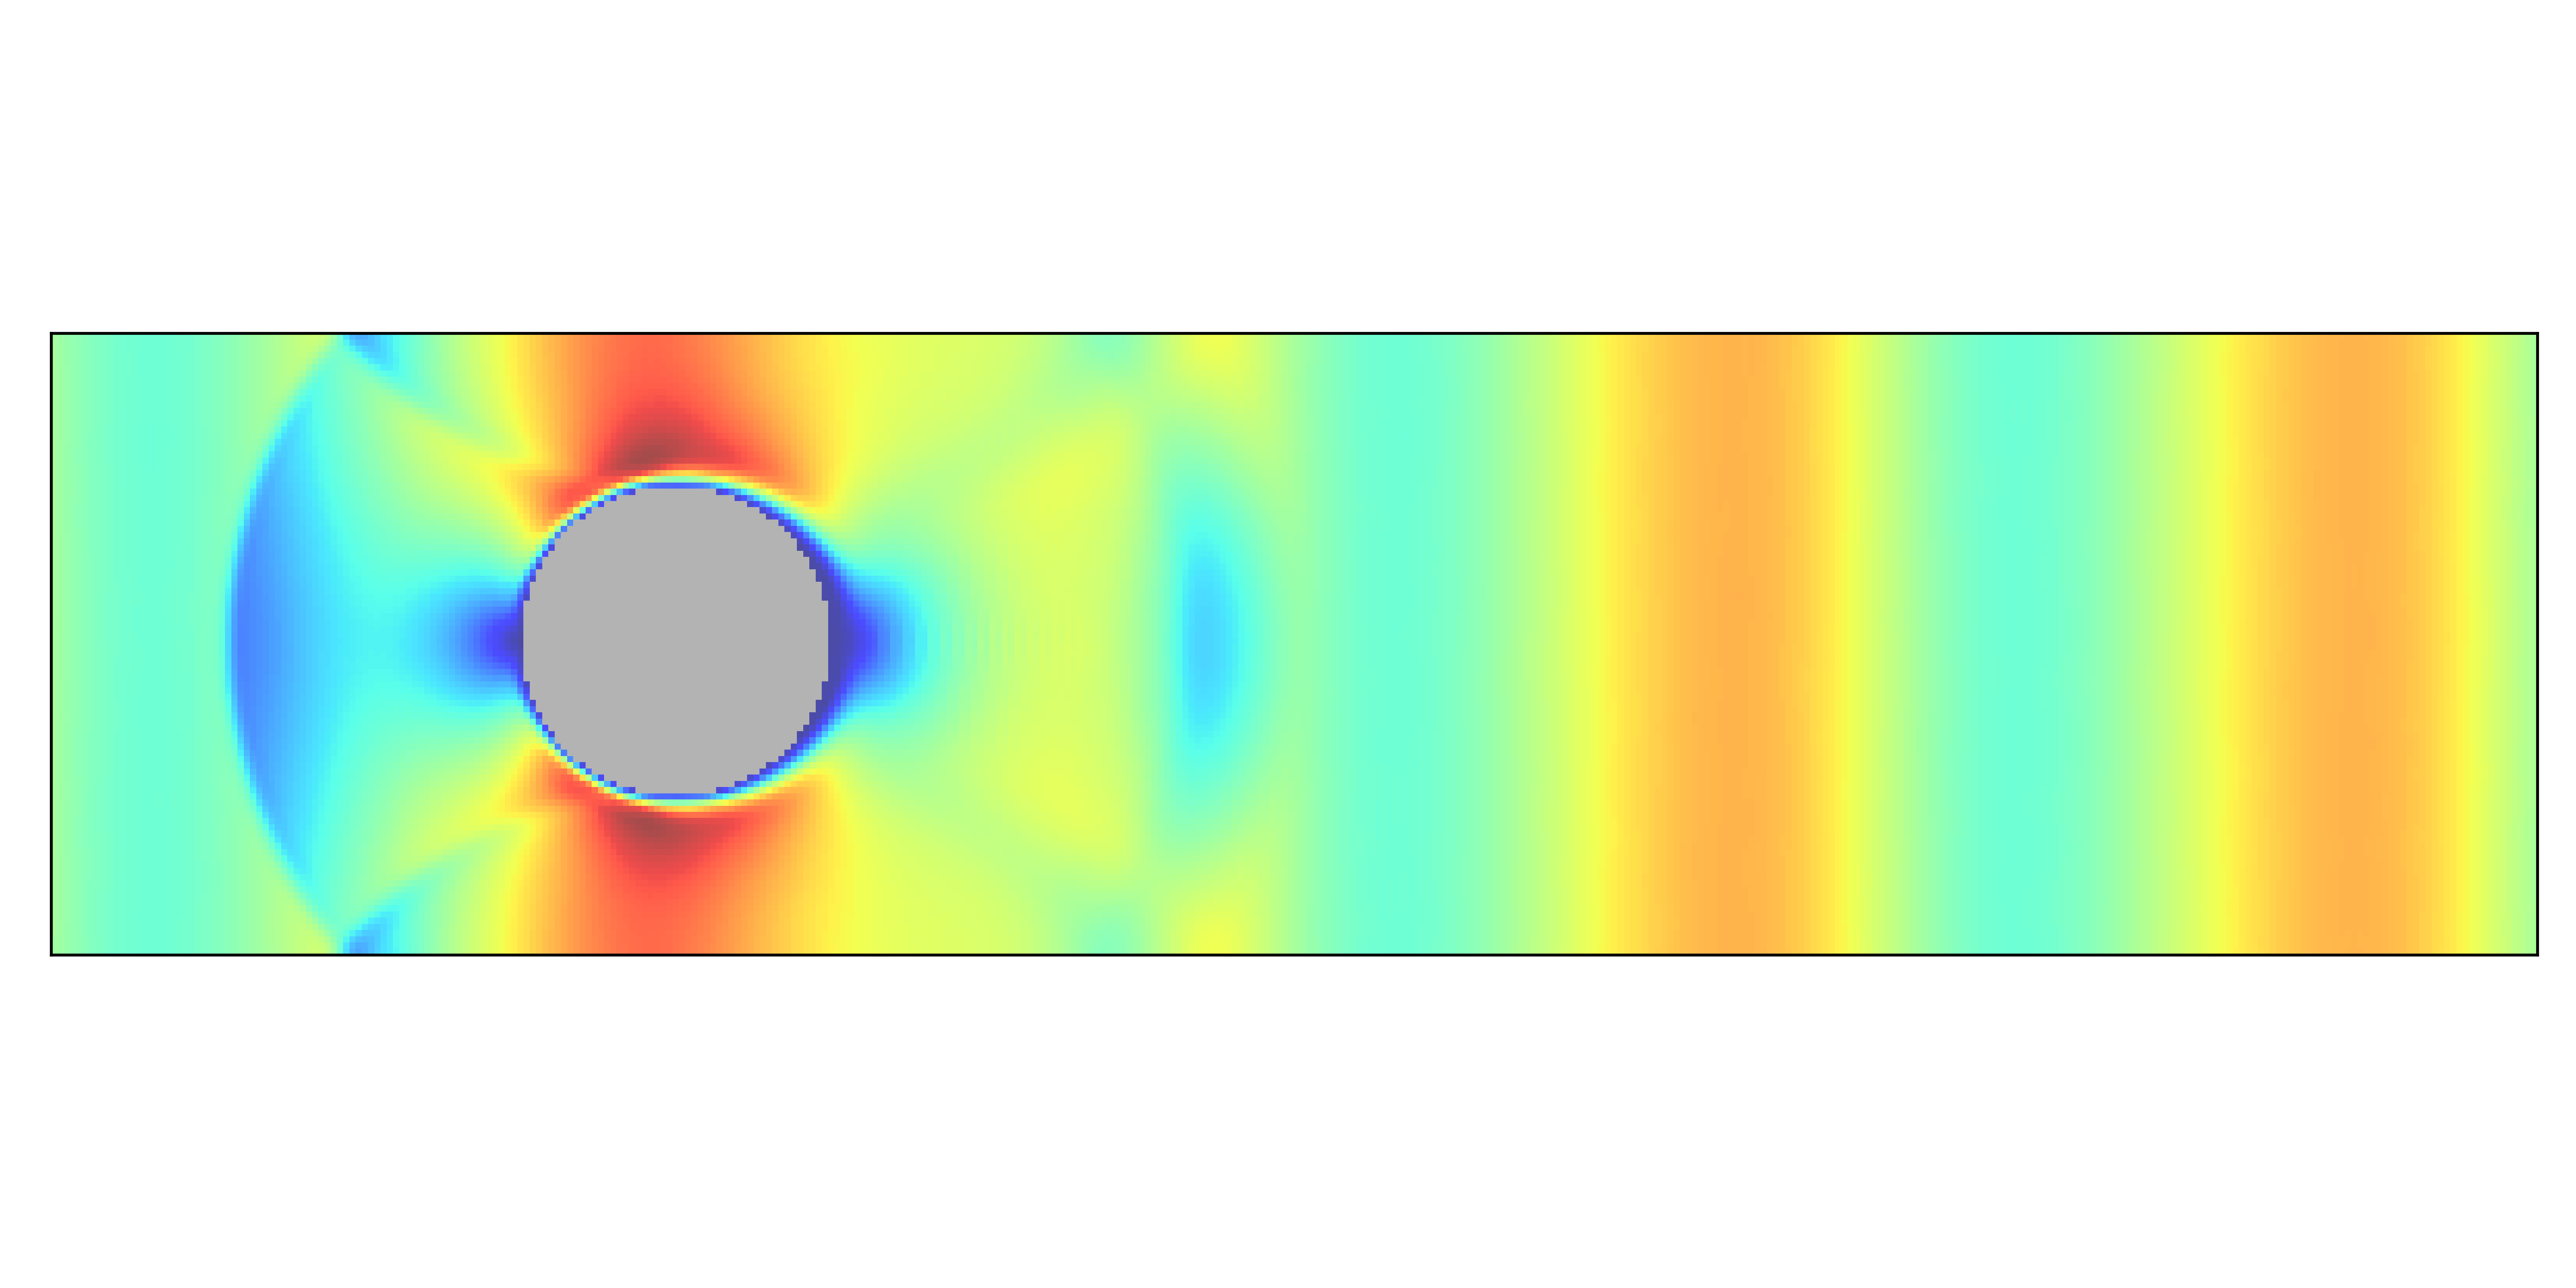
\includegraphics[scale=\myscale,scale=0.5,trim={0 3cm 0 3cm},clip]{figures/fluide-vitesse-100}
	
	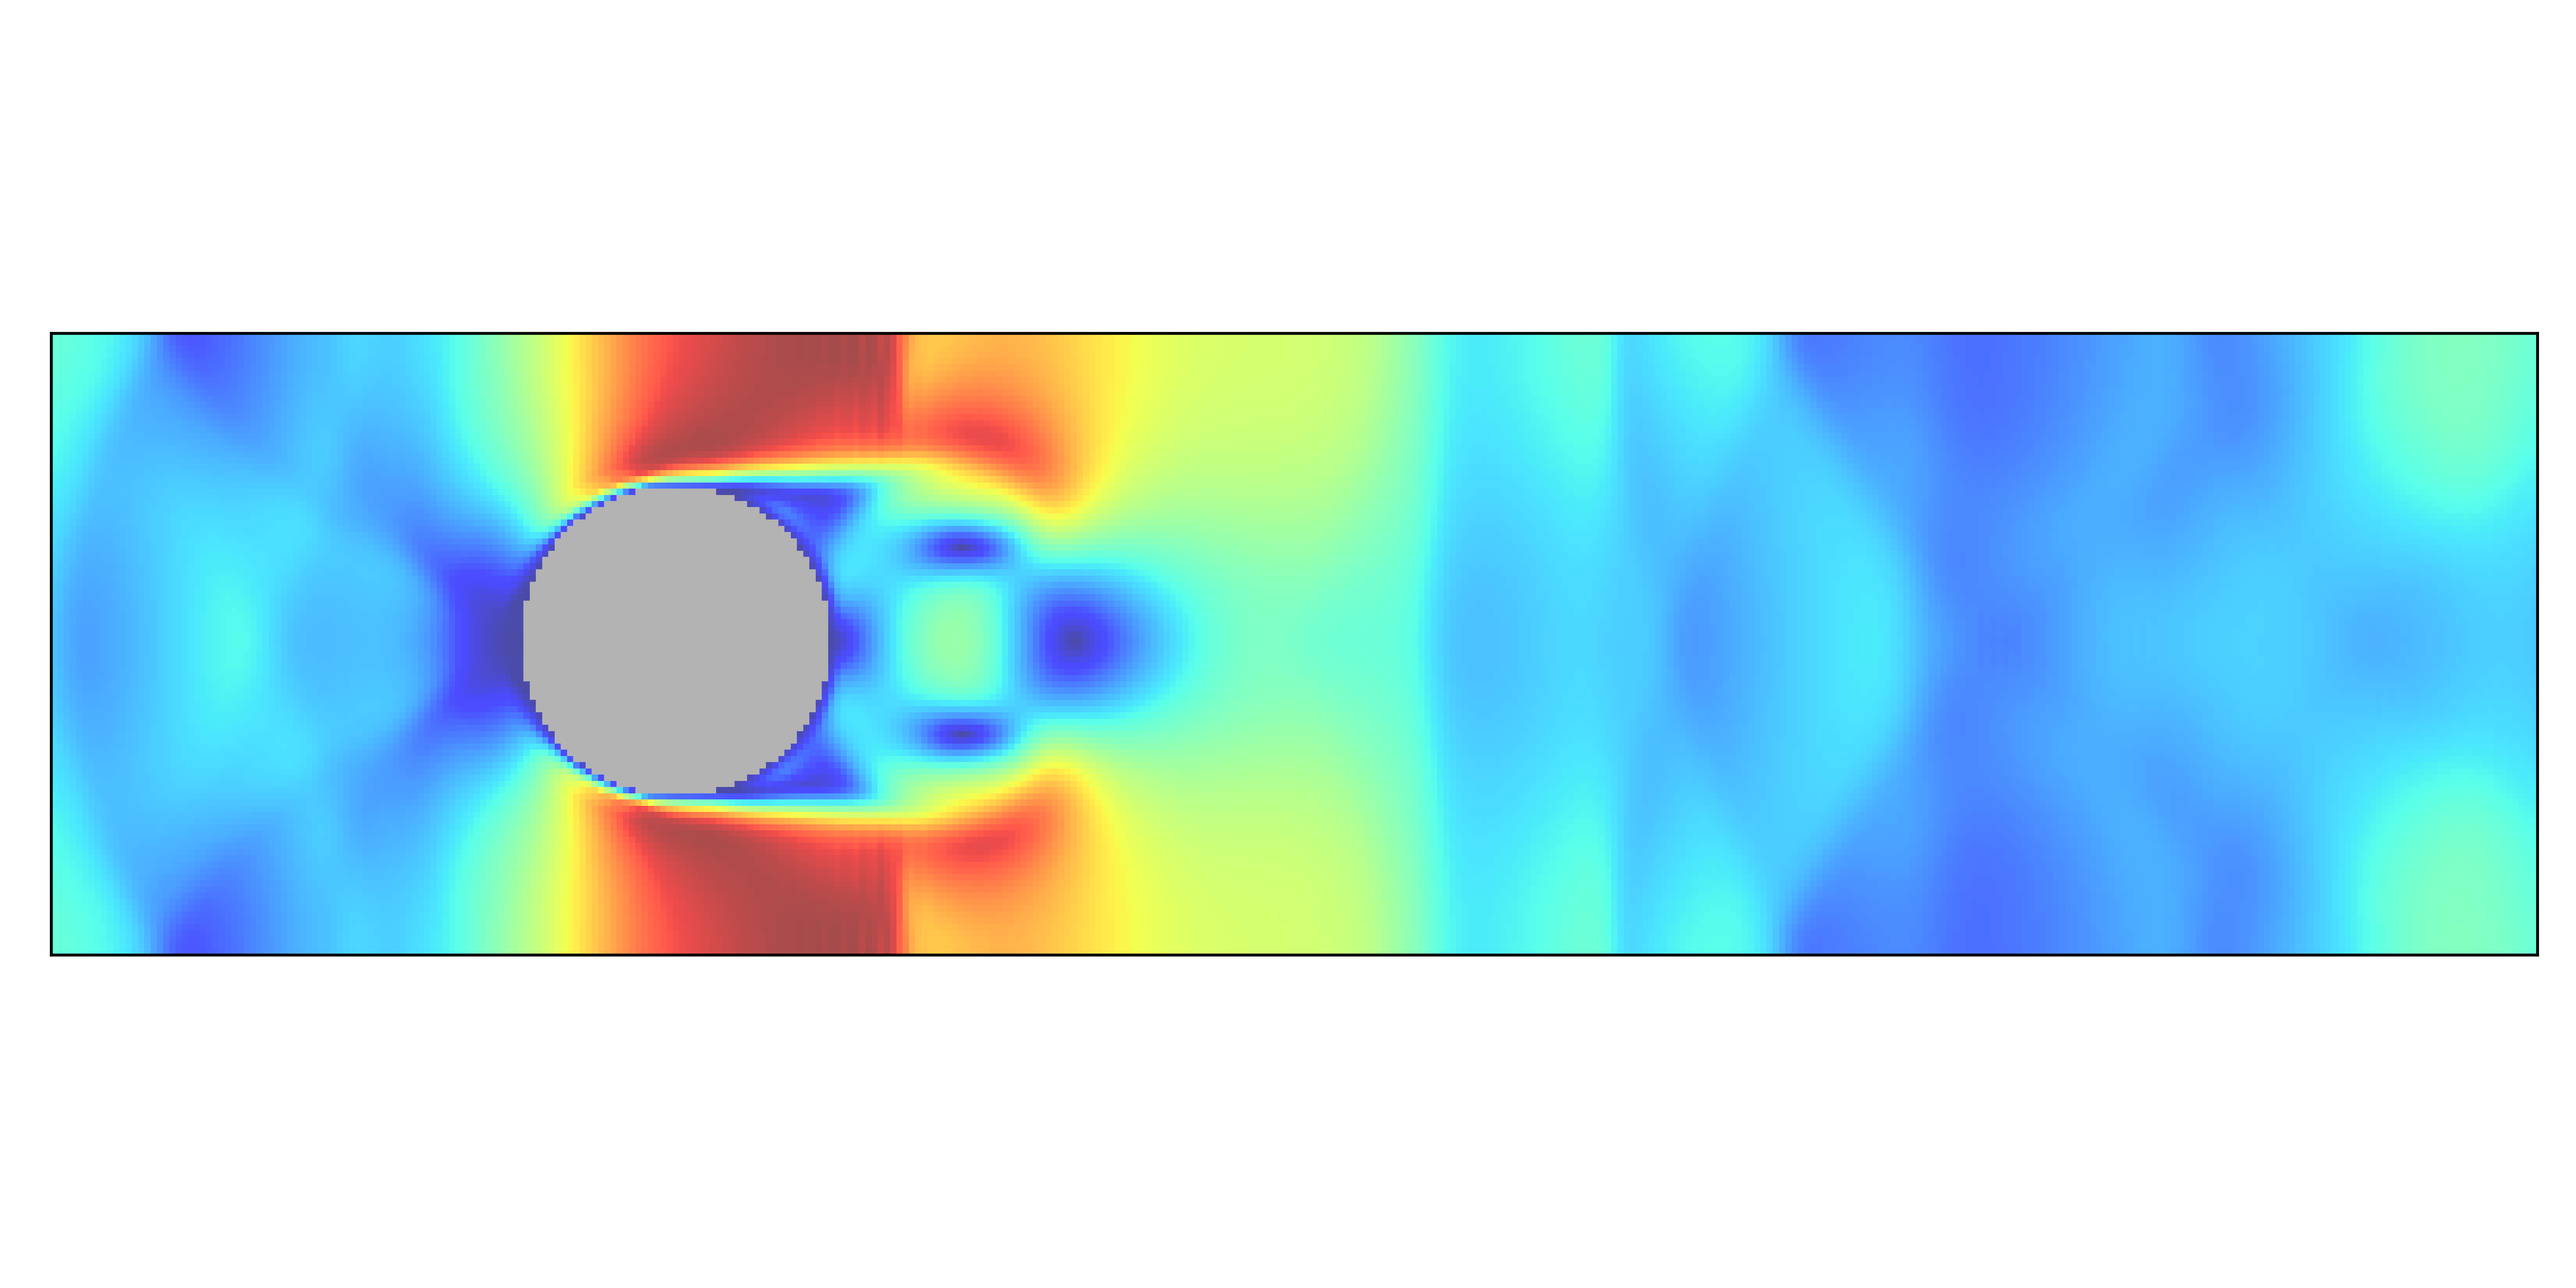
\includegraphics[scale=\myscale,scale=0.5,trim={0 3cm 0 3cm},clip]{figures/fluide-vitesse-500}			
\end{center}

Il faut noter que dans toutes ces simulations, on choisit de réinjecter par la gauche, le flux sortant du rectangle vers la droite. Ainsi la perturbation générée par l'obstacle finit par se faire ressentir devant l'obstacle après un certain nombre d'itérations.

 Ci-dessous la mesure de la densité $\rho(x,y)$ des particules après 100 itérations (en haut) et 500 (en bas). On note une densité plus forte devant l'obstacle qui s'explique par le rebond.
\begin{center}
	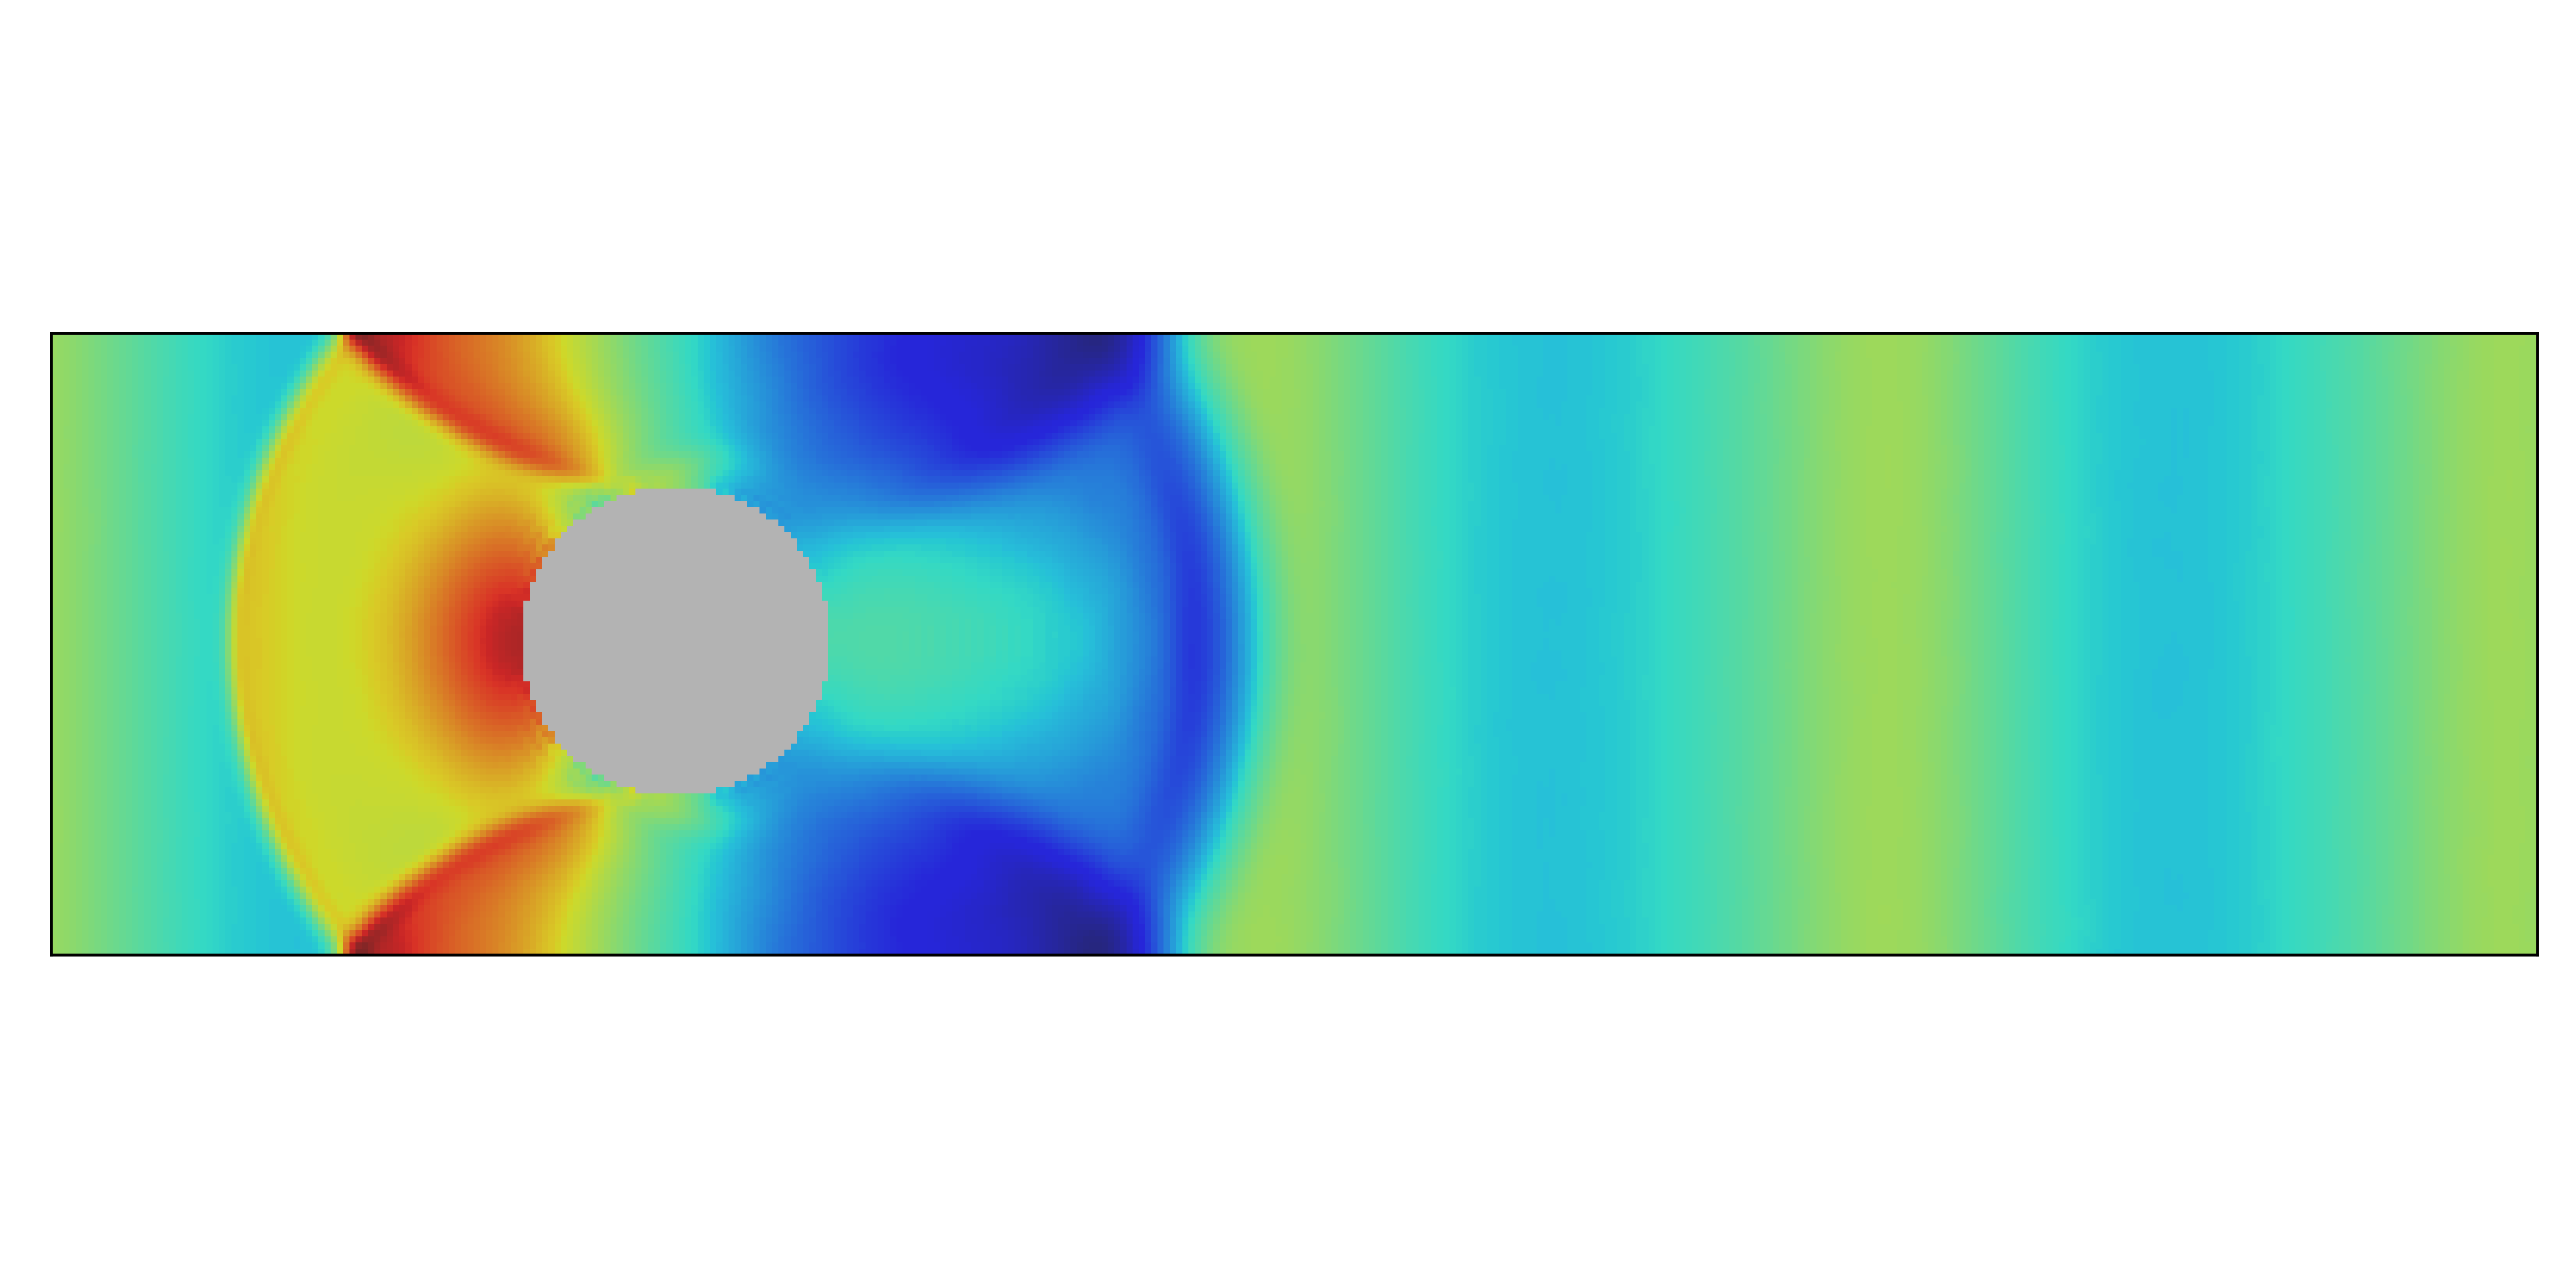
\includegraphics[scale=\myscale,scale=0.5,trim={0 3cm 0 3cm},clip]{figures/fluide-densite-100}
	
	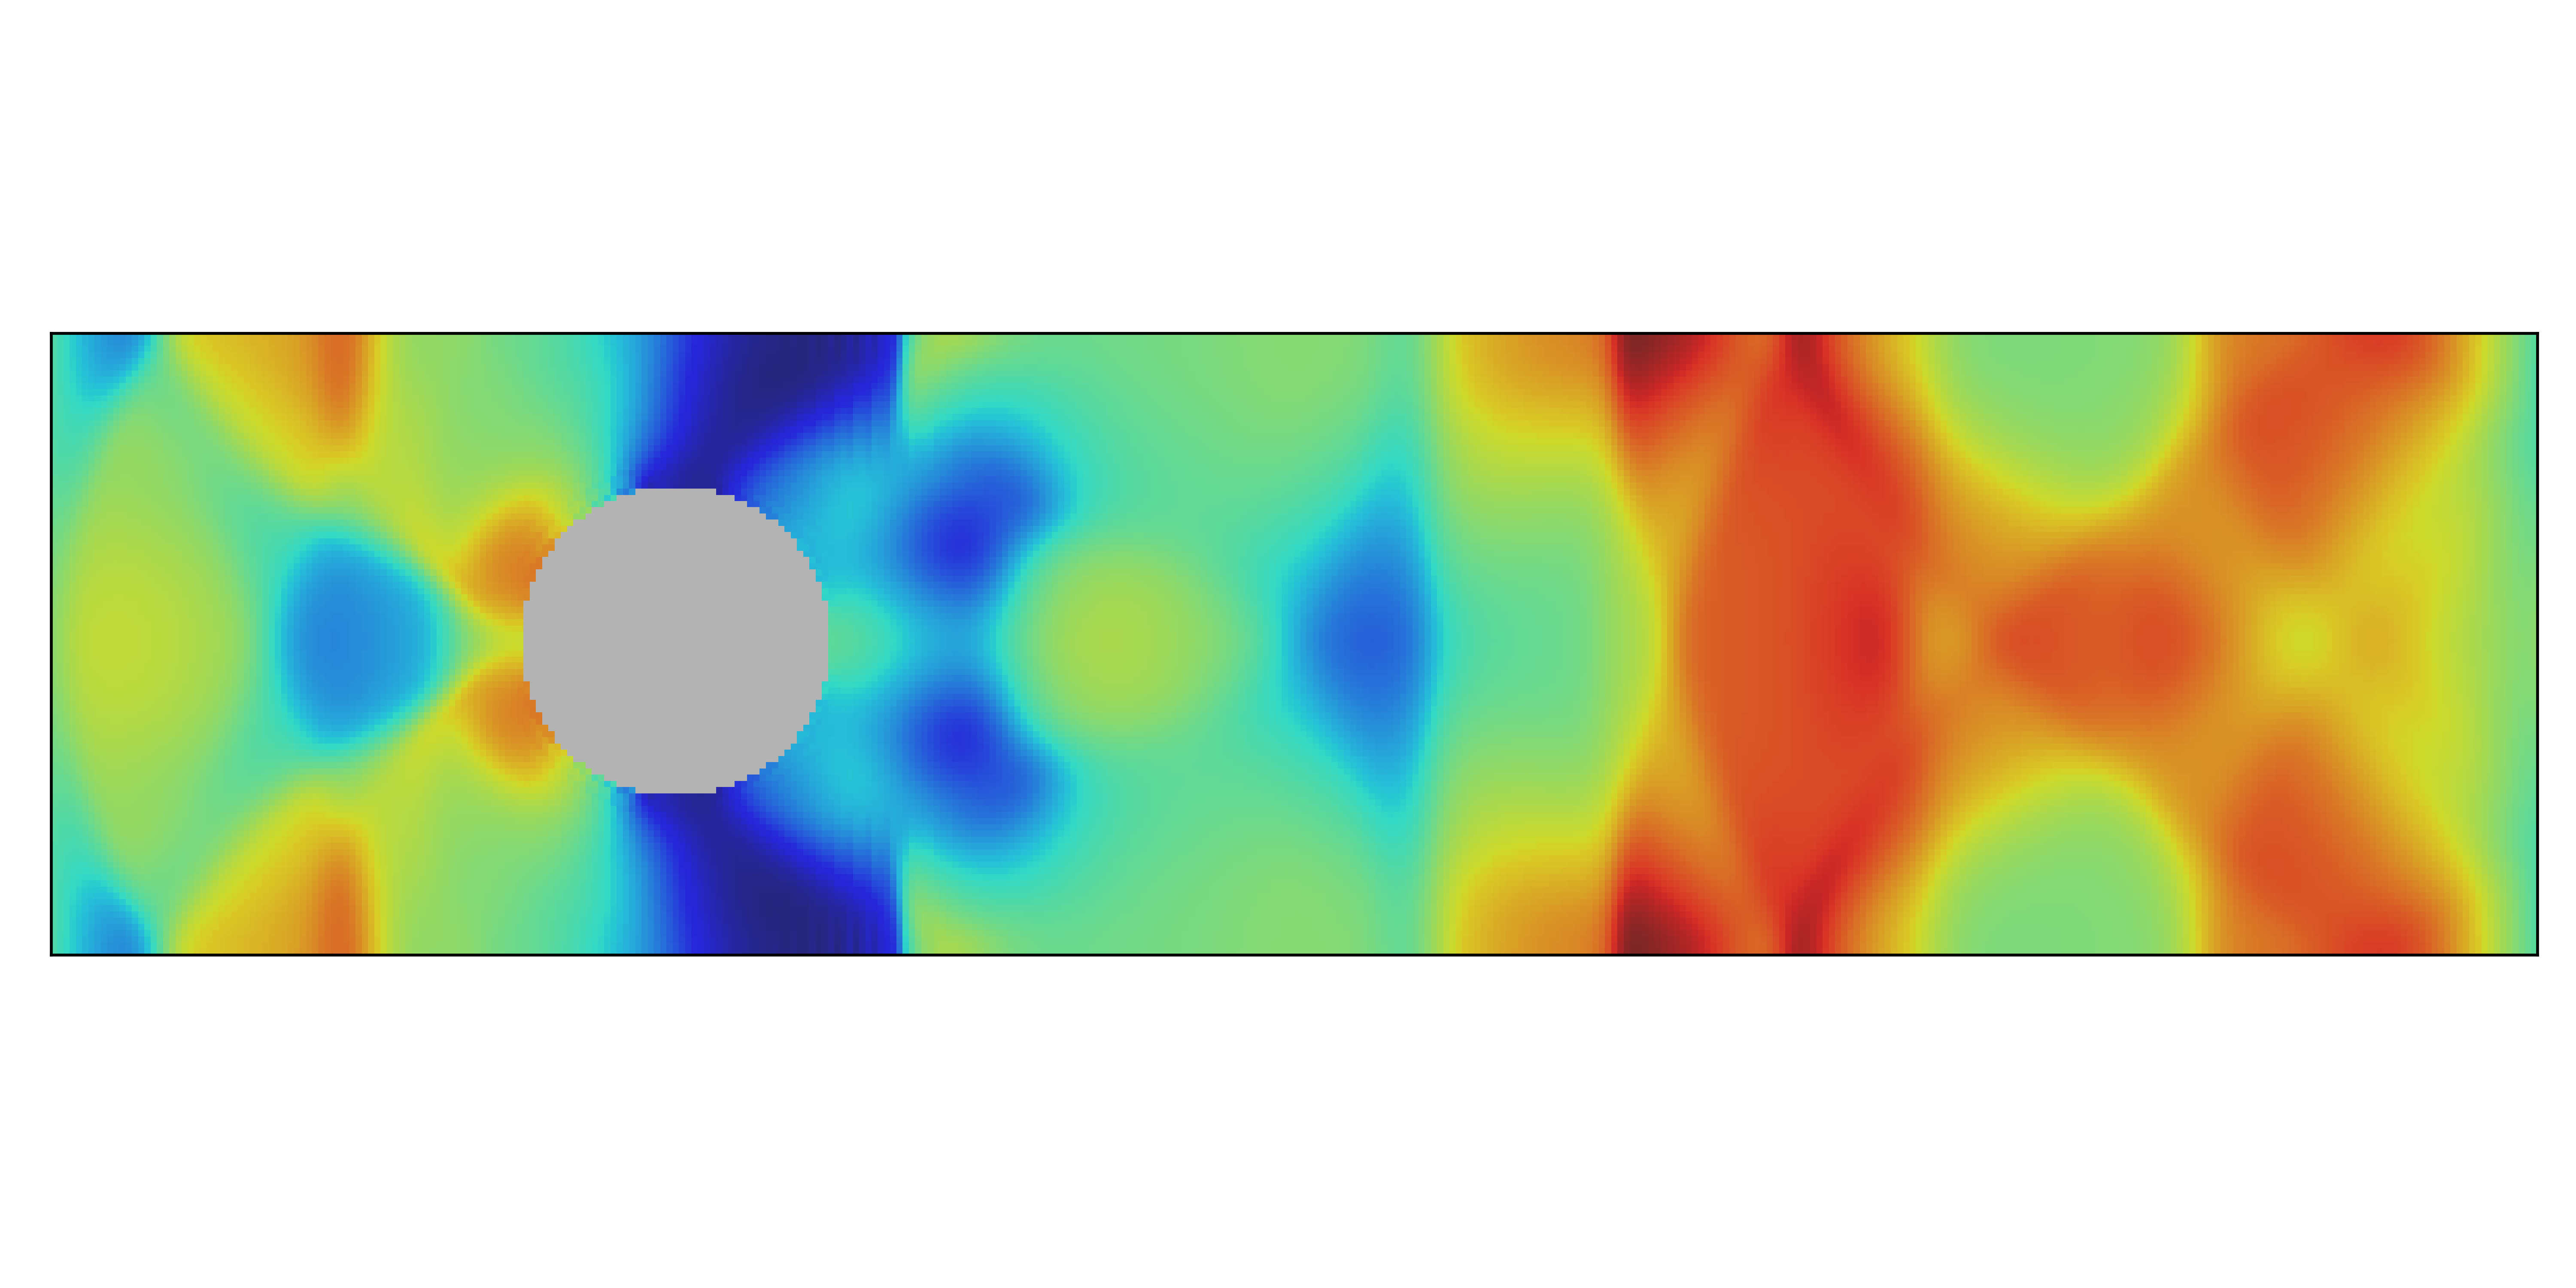
\includegraphics[scale=\myscale,scale=0.5,trim={0 3cm 0 3cm},clip]{figures/fluide-densite-500}			
\end{center}



%--------------------------------------------------------------------
\subsection{Vortex}

Les plus belles images sont obtenues en calculant l'effet vortex (\emph{vorticity}).
Ci-dessous le vortex pour $1000$ itérations. Les particules qui tournent vers la droite en se déplaçant sont \couleurnb{en bleu}{au-dessus}. Les particules qui tournent vers la gauche en se déplaçant sont \couleurnb{en rouge}{en dessous}.

%\begin{center}
%	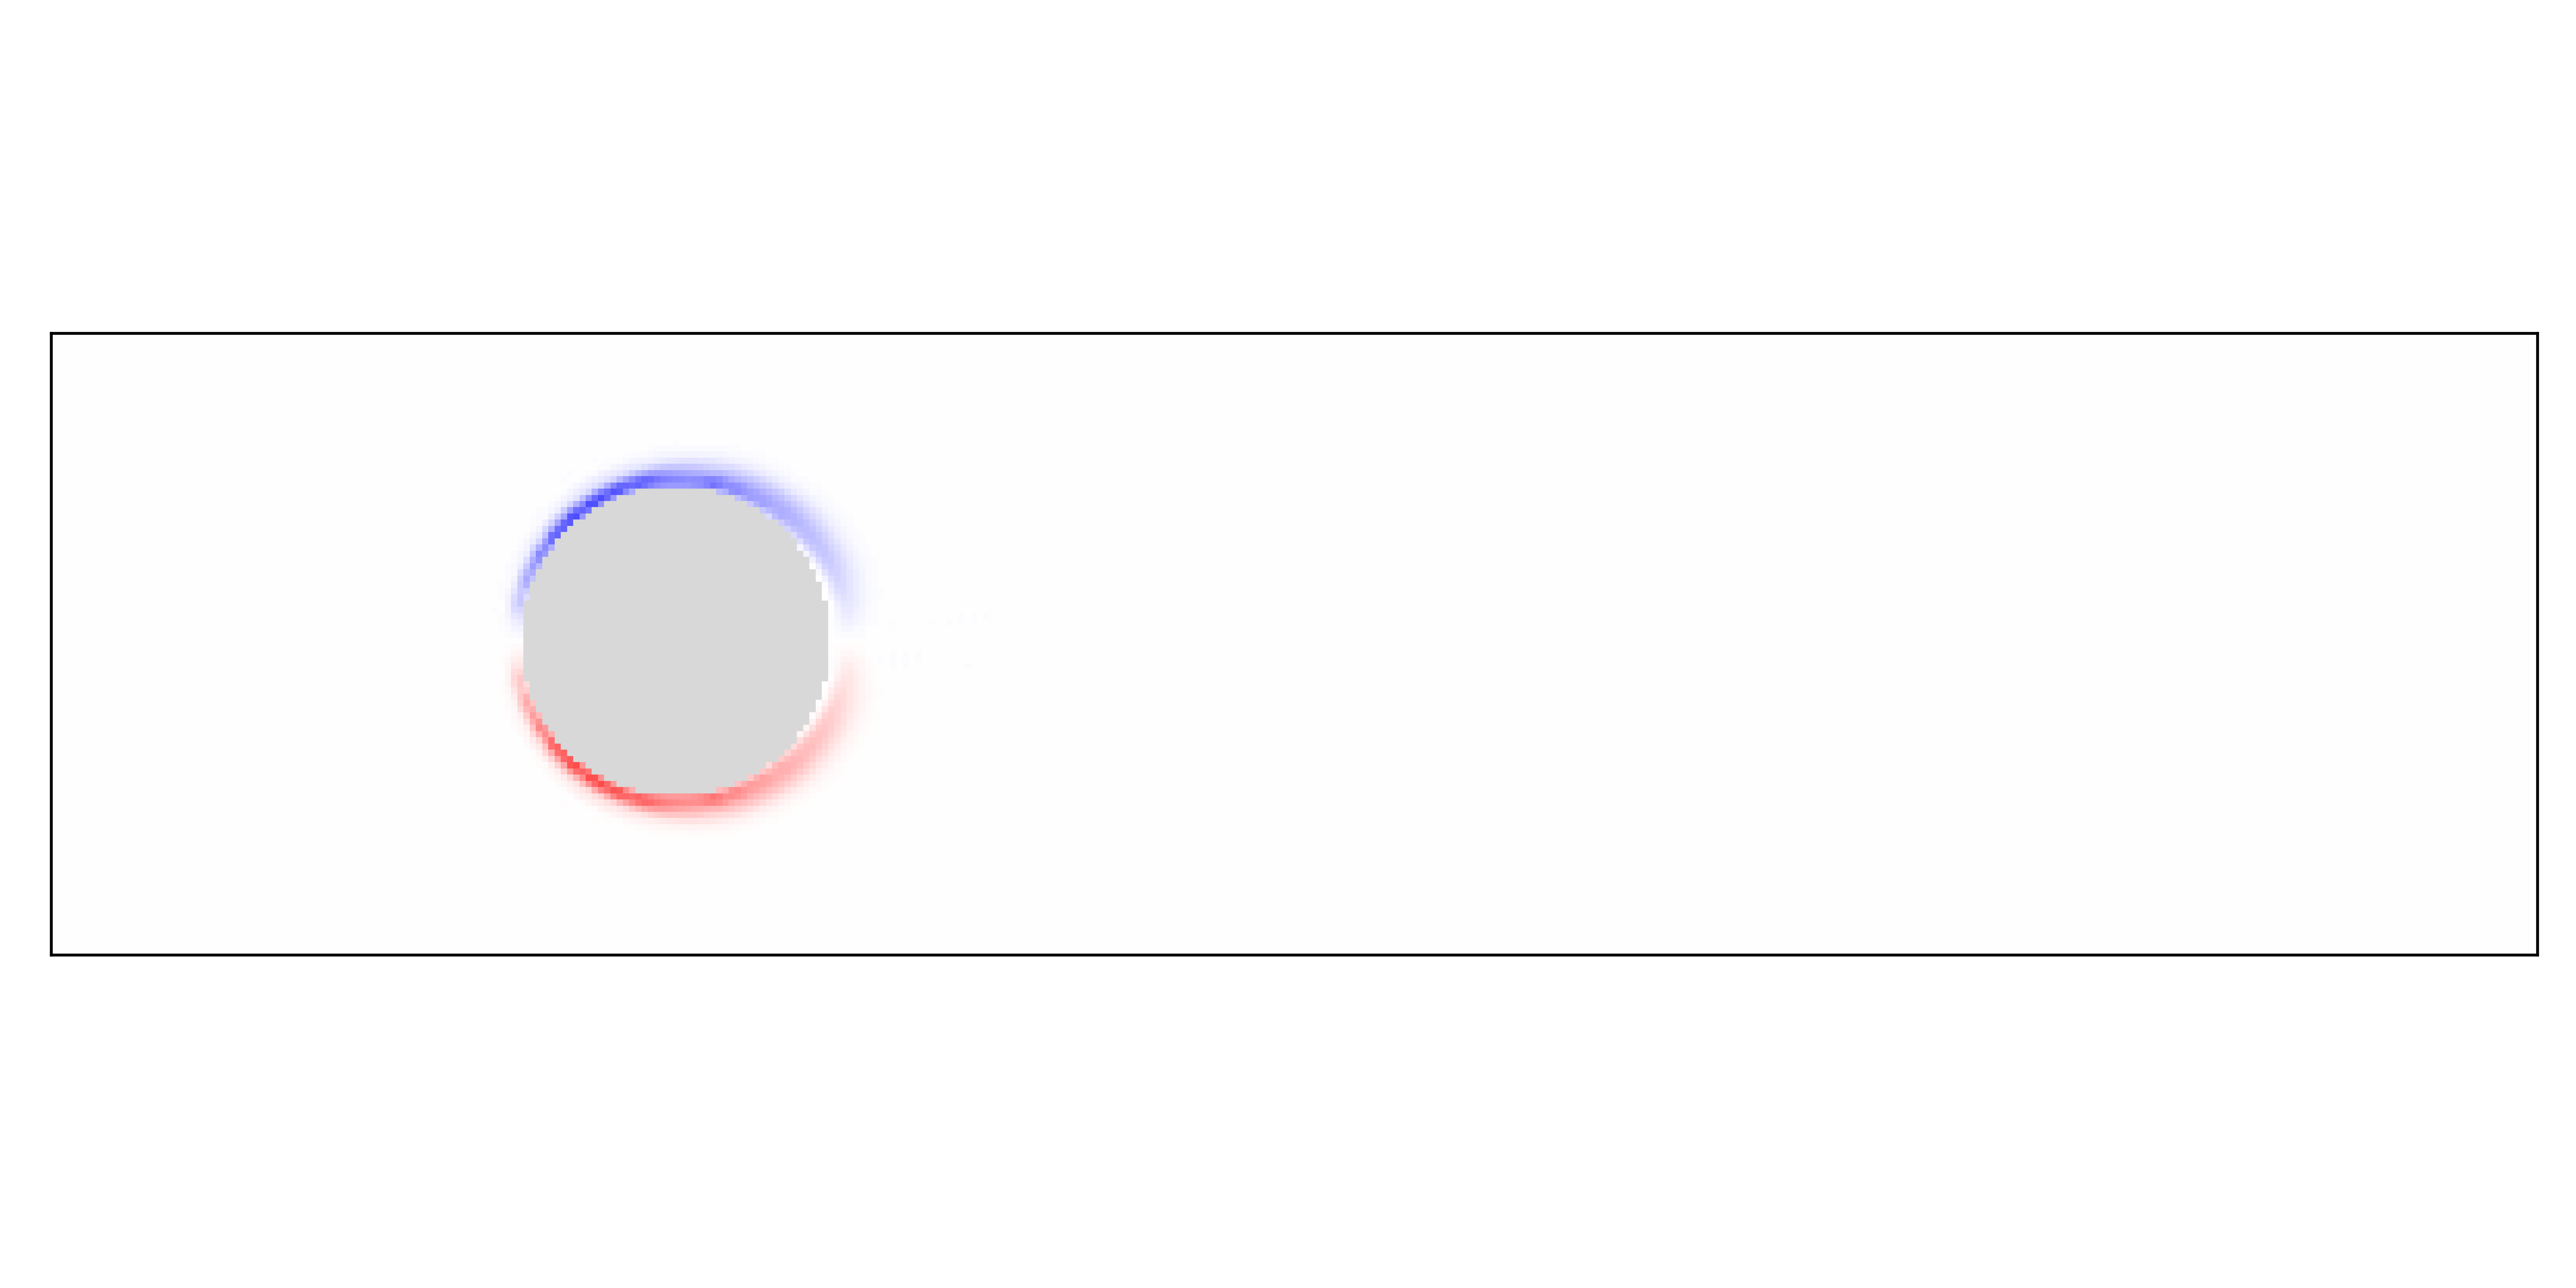
\includegraphics[scale=\myscale,scale=0.5]{figures/fluide-vortex-100}
%\end{center}

\begin{center}	
	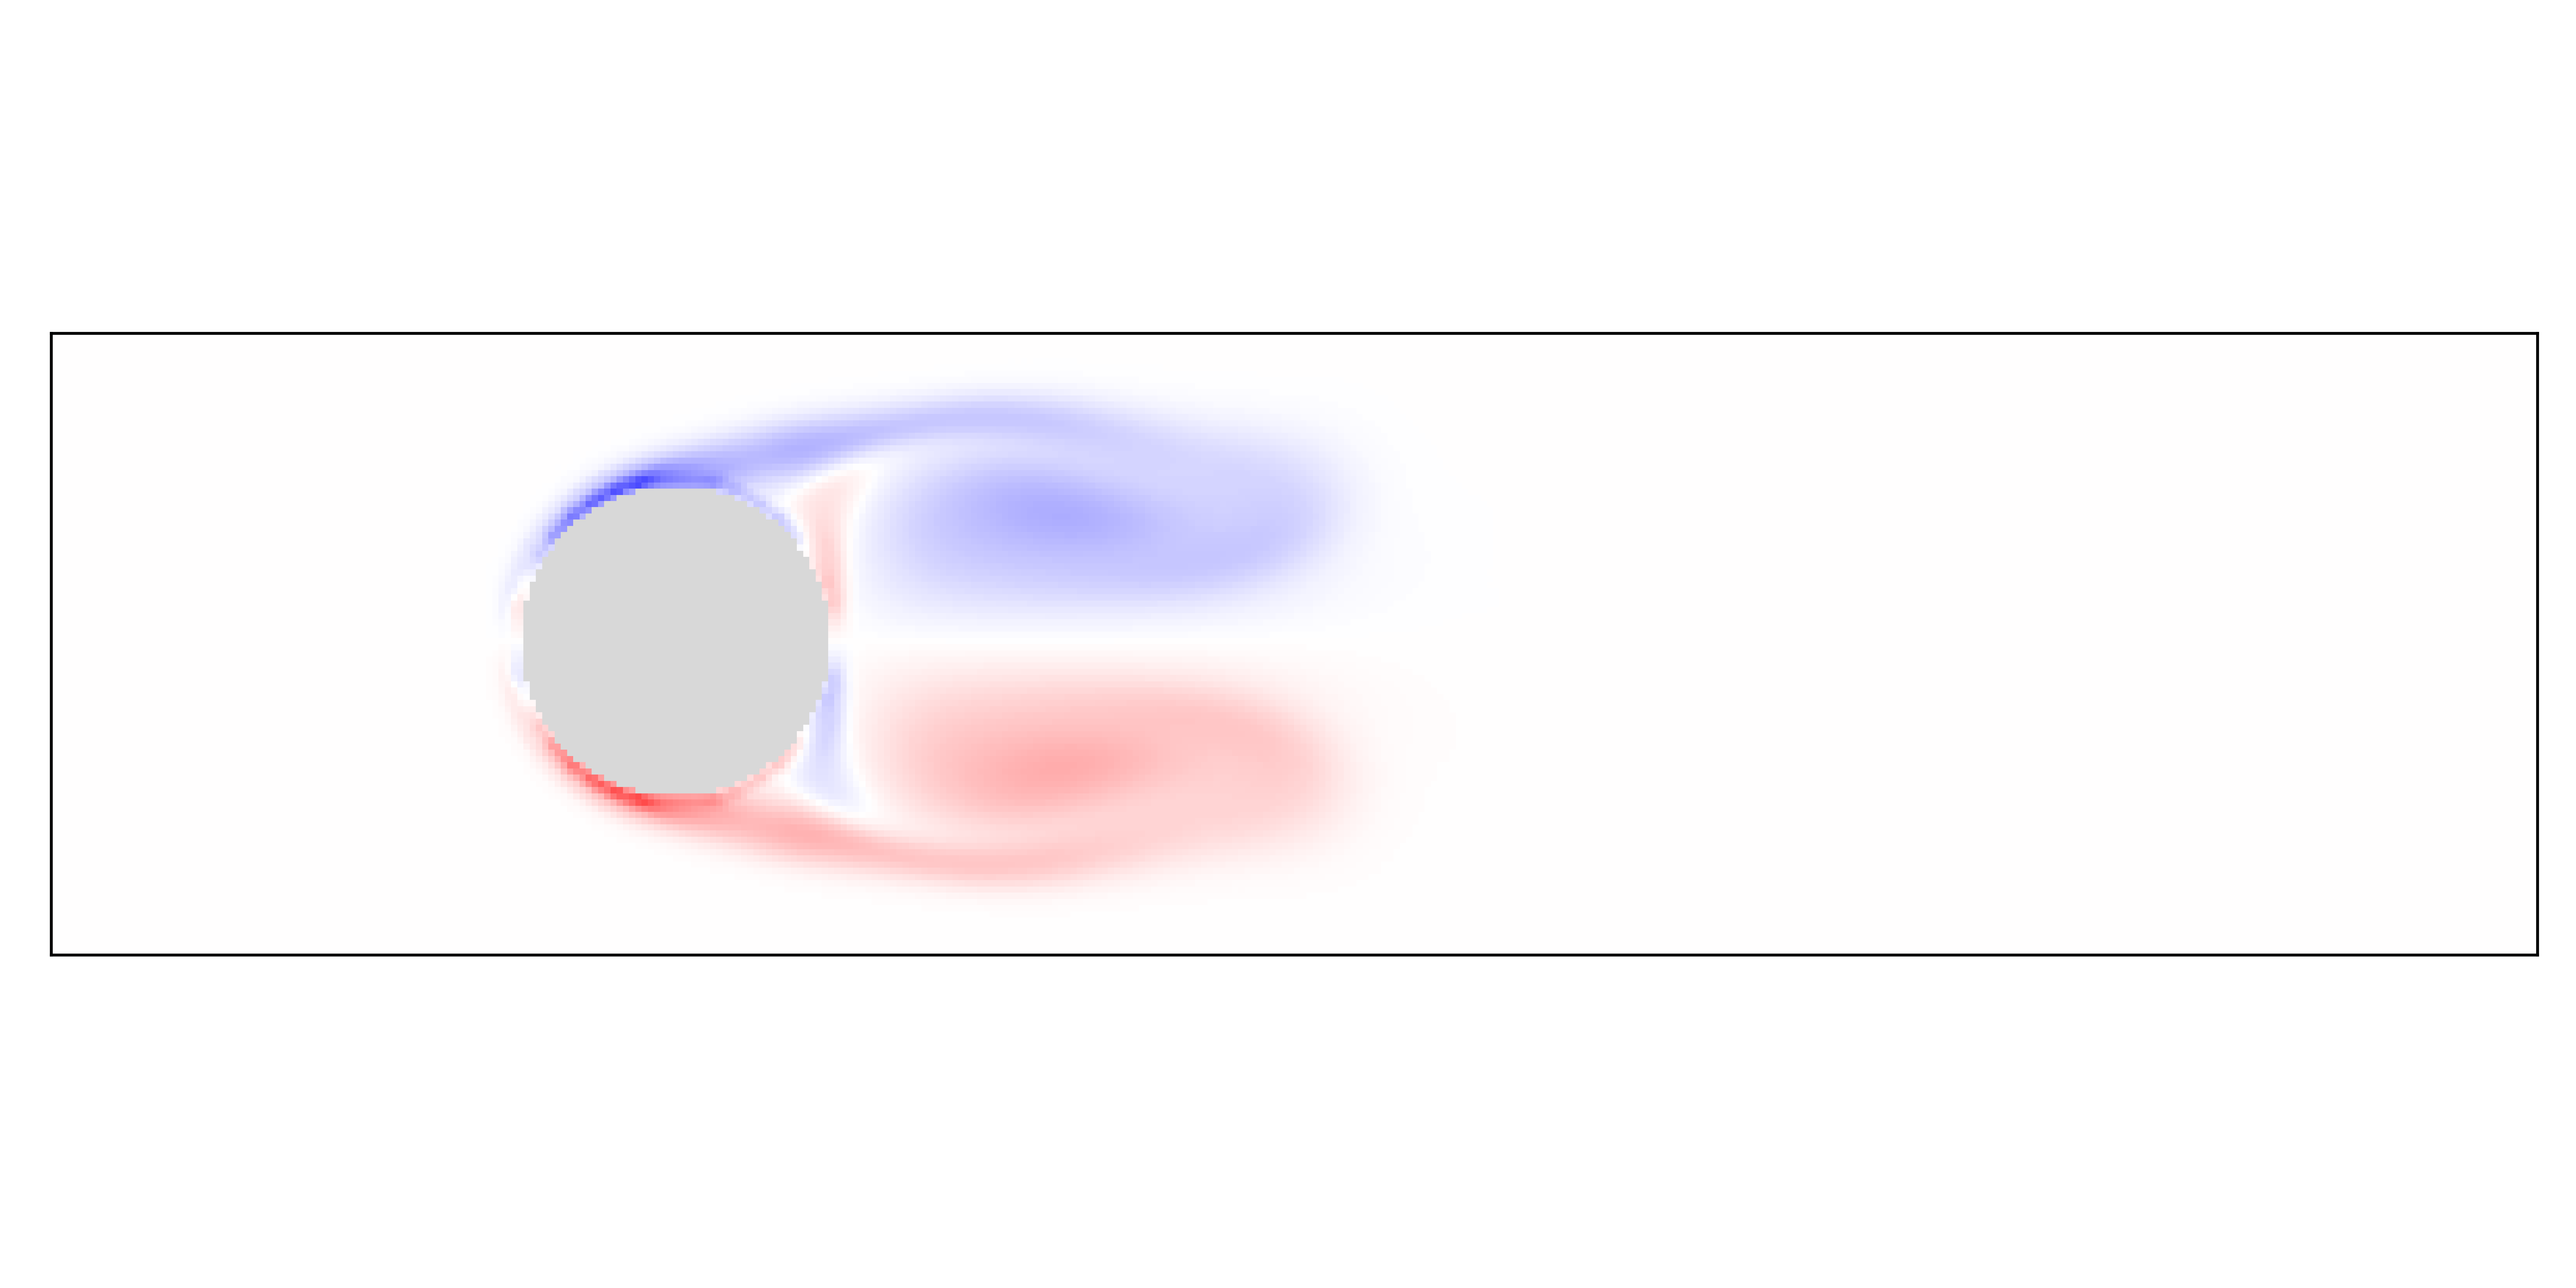
\includegraphics[scale=\myscale,scale=0.5,trim={0 3cm 0 3cm},clip]{figures/fluide-vortex-1000}			
\end{center}

Le \defi{vortex} se calcule selon la formule :
$$\omega(x,y) = \frac{\partial u_y}{\partial x} -\frac{\partial u_x}{\partial y}.$$
Le vortex mesure comment un petit ensemble de particules
tourne par rapport à son déplacement. Ci-dessous un petit carré qui contient plusieurs particules. Sur la figure de gauche il n'y a pas de vortex ($\omega=0$), à droite le carré tourne en se déplaçant, le vortex y est non-nul.

\myfigure{0.7}{
	\tikzinput{fig-fluide-10}
}

Pour calculer une version discrète du vortex on effectue :
$$\omega = \big( u_y(x+1,y) - u_y(x-1,y) \big) - \big( u_x(x,y+1) - u_x(x,y-1) \big).$$


Ci-dessous la situation au bout de 2000 et 4000 itérations.
\begin{center}	
	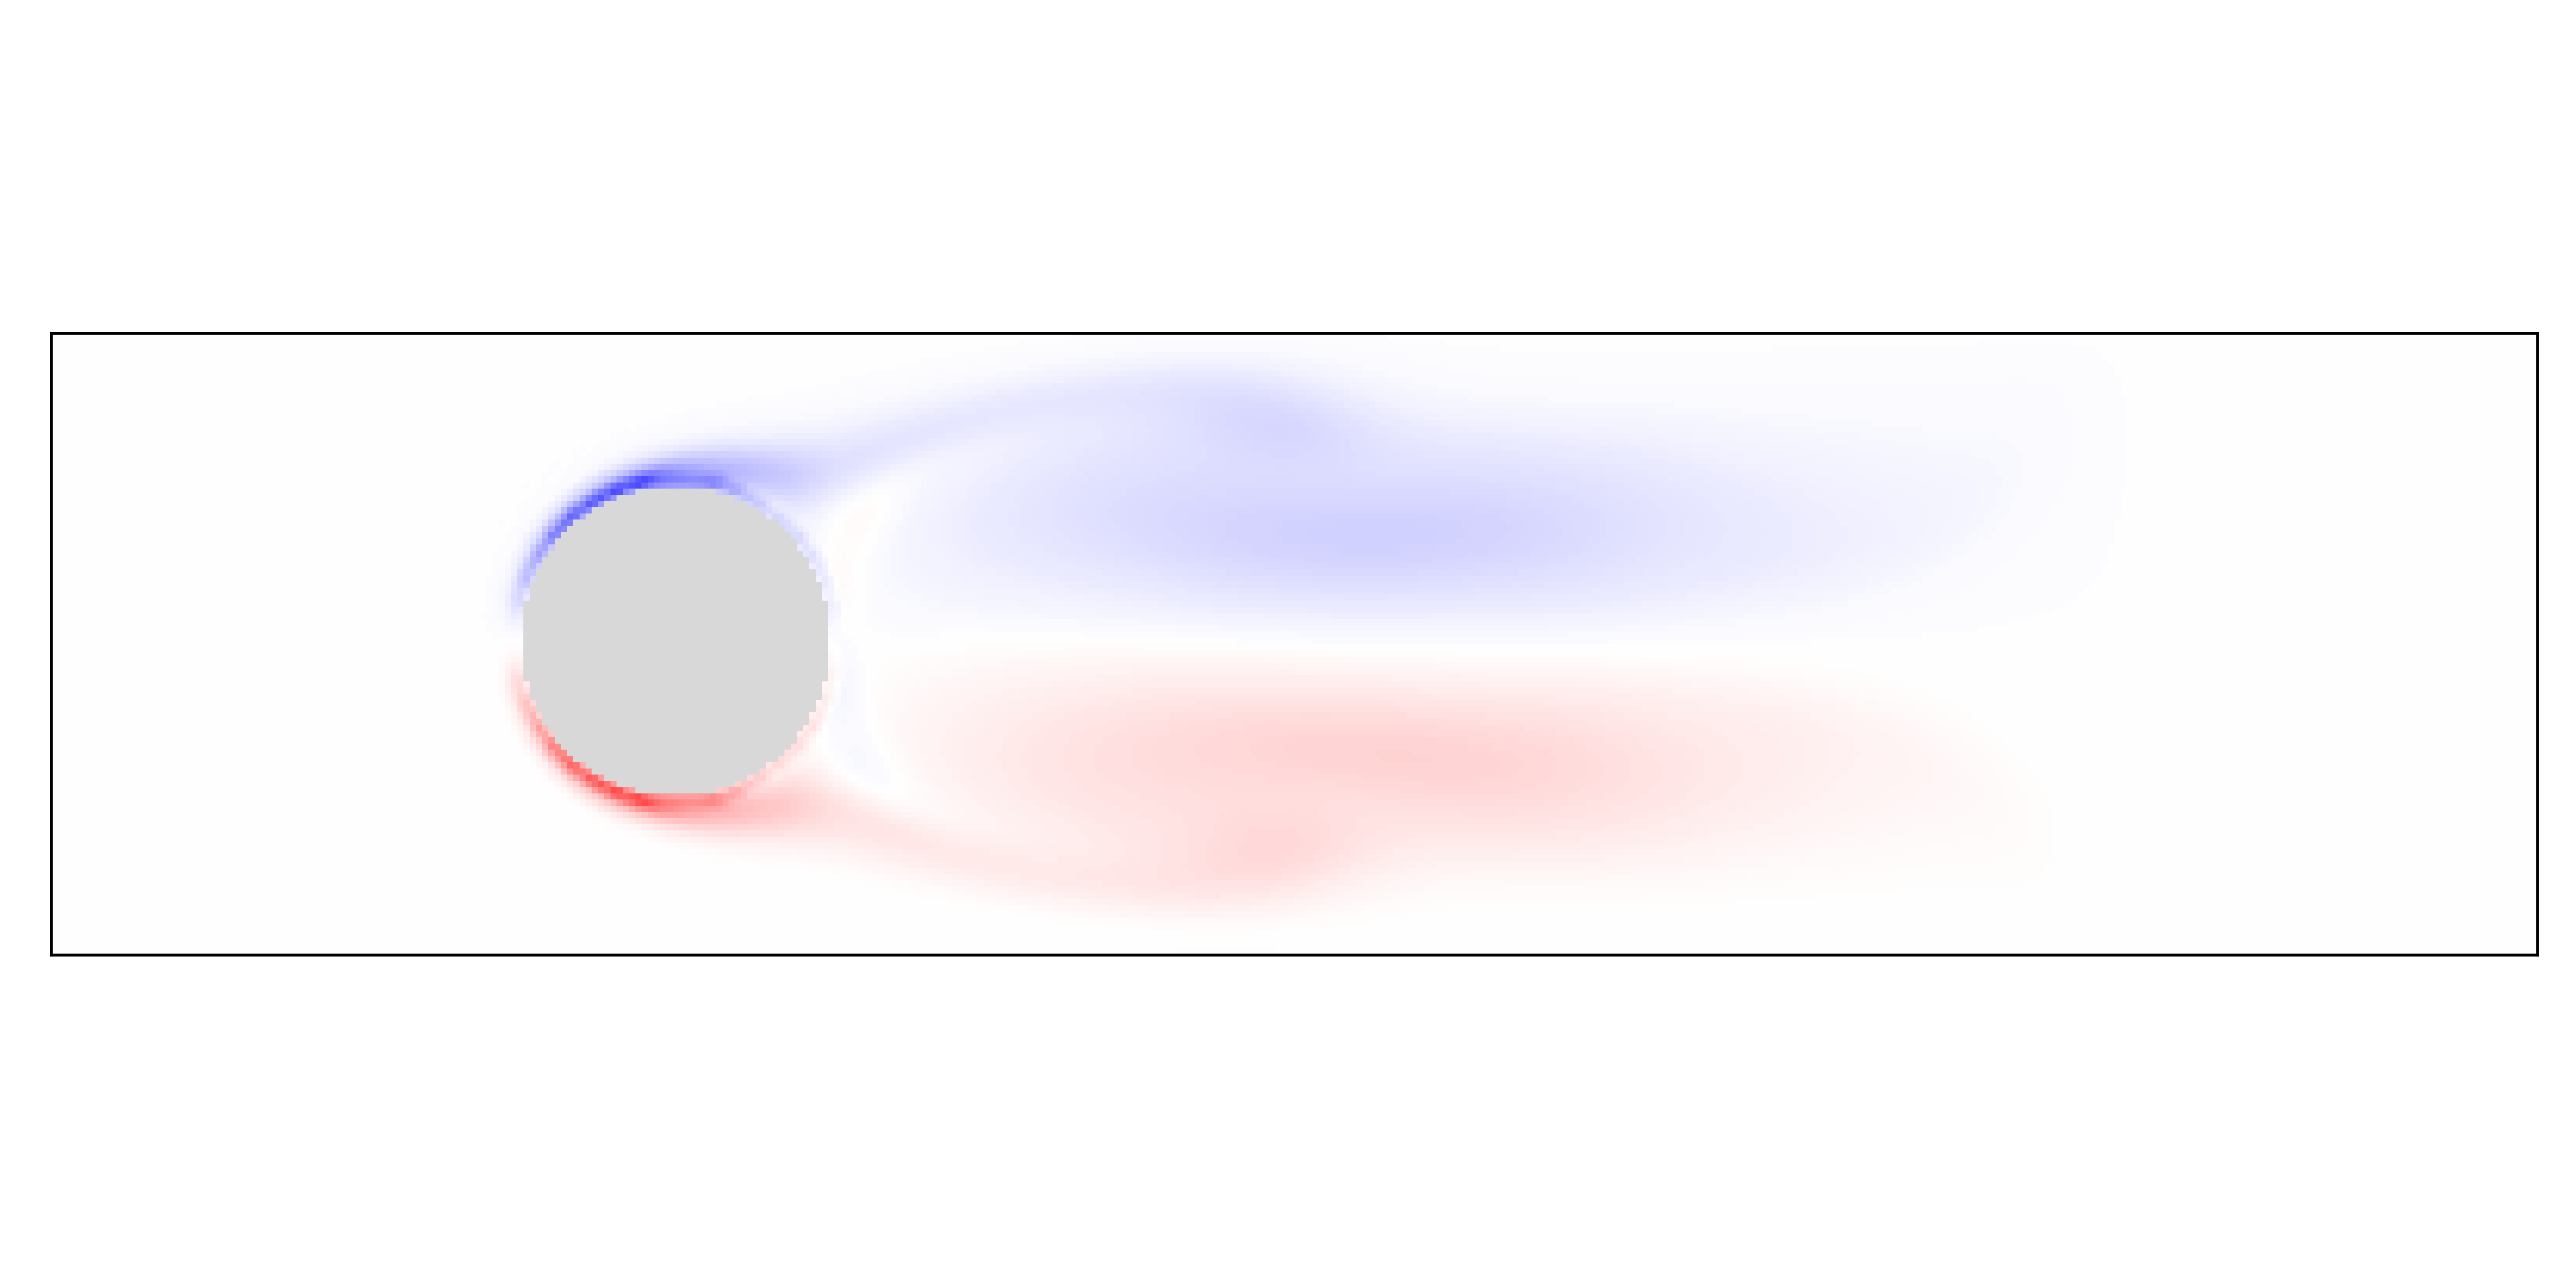
\includegraphics[scale=\myscale,scale=0.5,trim={0 3cm 0 3cm},clip]{figures/fluide-vortex-2000}			

	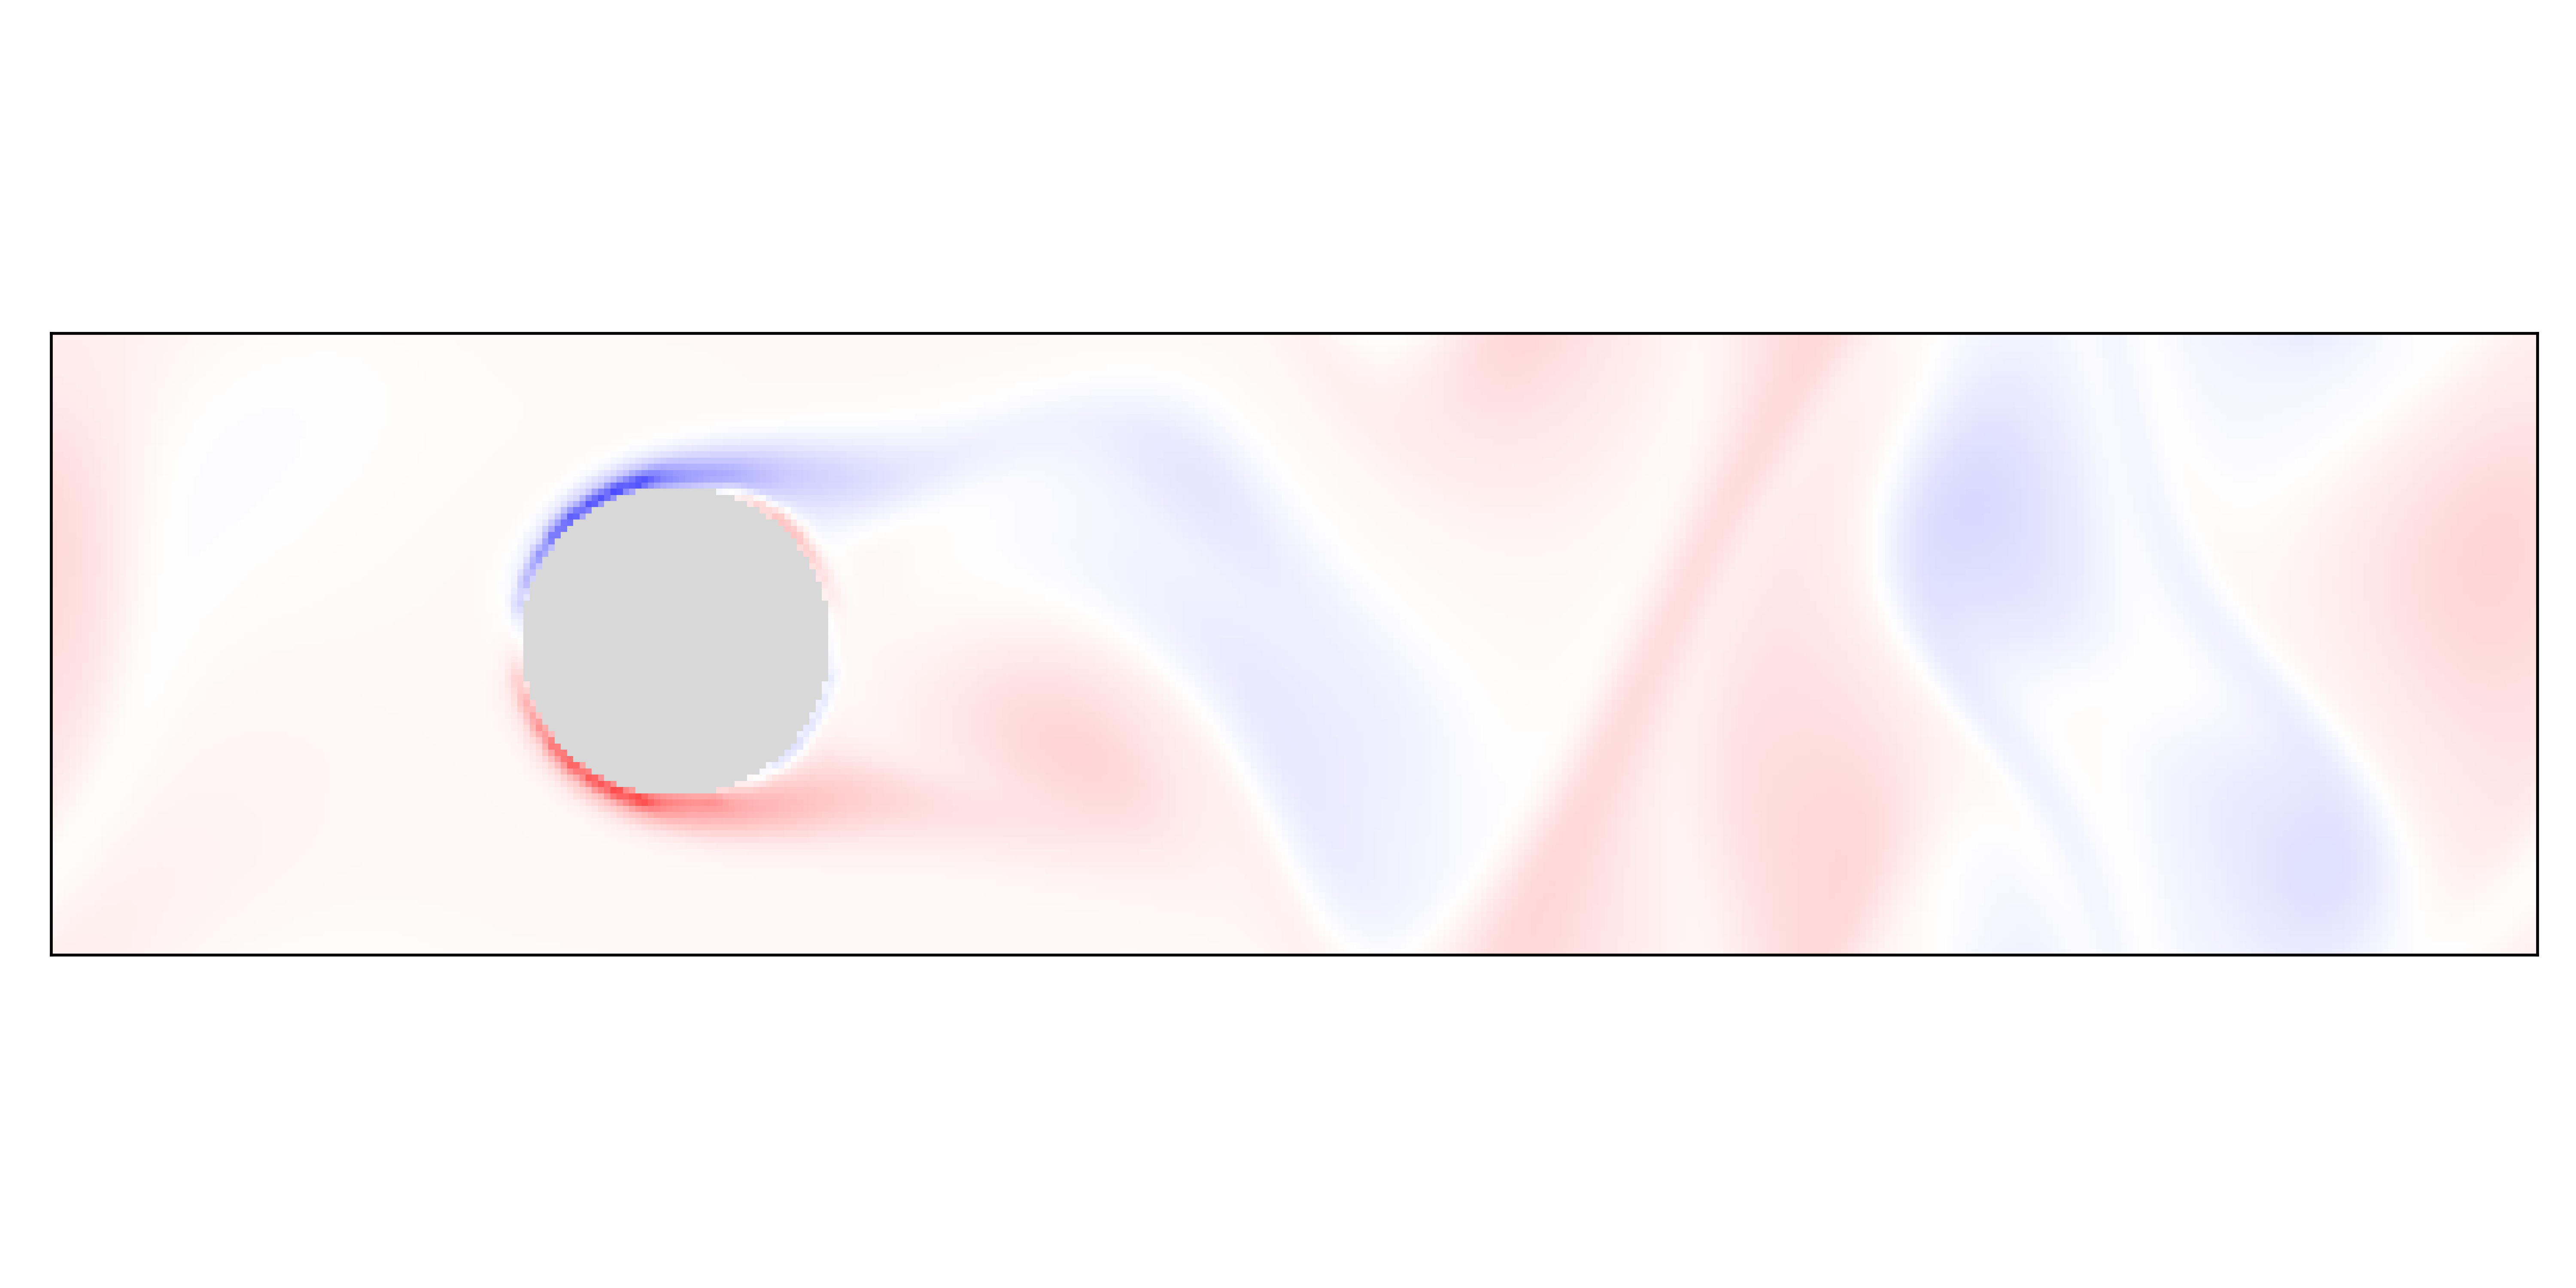
\includegraphics[scale=\myscale,scale=0.5,trim={0 3cm 0 3cm},clip]{figures/fluide-vortex-4000}			
\end{center}

\bigskip

Référence :  \href{https://medium.com/swlh/create-your-own-lattice-boltzmann-simulation-with-python-8759e8b53b1c}{\emph{Create your own lattice Boltzmann simulation}}
et  
\href{https://github.com/pmocz/latticeboltzmann-python}{page github}
de Philip Mocz.
La fonction d'équilibre qui y est présentée doit être corrigée en
$$F_{\text{eq}} (x,y,i) = w_i \, \rho \left(1 + 3 \vec{u} \cdot \vec{v_i}  +  \frac92(\vec{u} \cdot \vec{v_i})^2 - \frac32 \| \vec u \| ^2 \right)$$
 comme énoncée ci-dessus.


\end{document}